\chapter{Volume estimation}

Let me introduce to the topic of my PhD work at \acrfull{sk}.

\todo[inline]{TODO: complete chapter}

\section{Thesis Structure}
The diagram in \autoref{fig:thesis-structure} illustrates the flow of information through the structure of the thesis.

\begin{figure}[htb!]
\centering 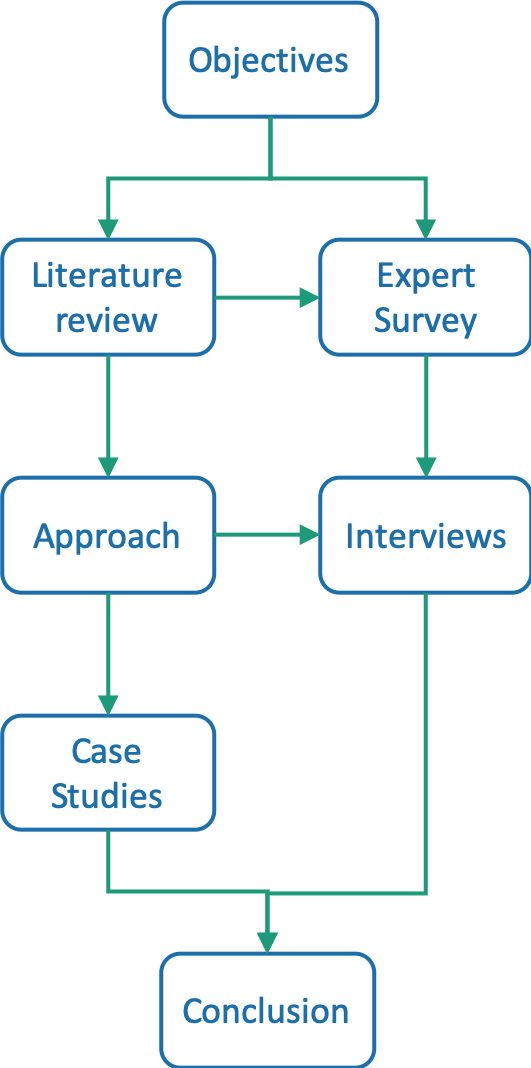
\includegraphics[width=0.5\textwidth]{graphics/thesis-structure}
\caption{Thesis structure}
\label{fig:thesis-structure}
\end{figure}

\begin{description}
    \item[\Autoref{cap:background} - Background]
Here's the literature review.

    \item[\Autoref{cap:thesis_objectives} - Thesis Objectives]
We define the objectives of our work.

...

    \item[\Autoref{cap:conclusion} - Conclusion]
In the last chapter, we discuss our results obtained ...
\end{description}

%%%%%%%%%%%%%%%%%%%%%%%%%%%%%%%%%%%%%%%%%%%%%%

Abstract. In this work a random sample consensus-based method of second order curve recognition is examined in terms of the dependency of the output quality on the intensity of noise in the input data. Specifically, the recognition method is applied to ellipses. The quality is evaluated the intersection over union between the real ellipse and the predicted one. The results quantitively describe the dependency of the output quality on the characteristics of input data, suggesting deterioration of the model as the data becomes more and more noisy. A series of numerical experiments is conducted on challenging synthetic data.
INTRoDUCTION
Curve recognition and shape recognition is an important part of many modern industrial applications. In particular, ellipses are used to approximate the section of a tube, human head, and other objects that appear as ellipses [1]. Real-world 3D circles appear as ellipses to a tilted camera, and its parameters provide information about the position, distance and the inclination angle of the said circle.

There is a number of approaches to the shape recognition problem. The most widely used include least squares method, Hough transform and RANdom SAmple Consensus(RANSAC) [2]. Let us briefly cover the main features of these approaches. First of all, least squares method is simple, straightforward, fast, easy to interpret. It relies on the quadratic error function that is differentiated with respect to the model parameters. It results in a set of equations that could be solved for the values of the parameters that minimize the quadratic error. While this method is widely used, it has certain drawbacks. The main one is that this method lacks robustness to noise. If presented with a data with a small portion of strong outliers, least squares method will incorporate those outliers in the calculation of the optimal model parameters, which significantly degraded the quality of the output model. Consequently, least squares methods cannot be used if significant noise is present.

In the 1960s, when modern computers started to appear in research institutions, a novel approach to data analysis was invented. It was widely adopted, previously being unusable by human workers because of heavy computational burden that should be carried in order for this method to work. This method goes by the name of Hough transform. In contrast to the previously mentioned least squares method, this approach relies on the explicit formation of the discretized parameter space for all the possible models. For such objects as lines the dimensionality of the parameter space is two if these lines exist on the two-dimensional plane. For such objects as circles or parabolas the dimensionality of the parameter space will be equal to three. For such objects as ellipses the dimensionality of the perimeter space will be equal to five.

Hough transform algorithm works as follows. First, a so-called accumulator is created. The dimensionality of this array is equal to the number of independent parameters in the model. It is usually set to be an array with the integer elements. For instance, for circles, it will be a three-dimensional array. Each of the axis will represent x coordinate, y coordinate and the radii of the circle, respectively.

After the accumulator is formed, the main loop begins. It consists of iterative going through all the input data points. For each of them all the possible models are considered that go through that point. A discrete step corresponding to the discretization of the accumulator array is used. For two-dimensional lines a number of the possible models is proportional to Pi over the discretization step. For circles there are two different discretization steps, resulting in the quadratic number of possible models. It could be noted that with the growth of the dimensionality of the model, the size of the accumulator and the number of iterations grow rapidly. Consequently, for five-dimensional surfaces and curves applying classical Hough transform becomes infeasible.

The input of all these algorithms is a number of two-dimensional points, and the output of the algorithm for ellipses are five parameters, namely two coordinates, two semiaxes, and the rotation angle. The standard way of using ellipse recognition approaches is the following. First, an image is taken with the robot’s onboard camera or other imaging device. Second, the image is segmented. Third, the part of the segmentation mask that corresponds to the ellipse is processed in order to decrease the number of pixels in. Finally, all the points are fed into the recognition algorithm.

Random sample consensus is a de-facto standard for a number of computer vision problems, including perspective transform evaluation, 3D reconstruction[3], and pose estimation. A number of works were devoted to the evaluation of the influence of the noise on the output quality[4]. However, RANSAC is not a single algorithm, it is rather a family of algorithms with their performance, speed, complexity, and convergence, depending solely on the class of the models considered[5], [6].

In this work, a systematic approach is taken towards examining the performance of the random sample consensus approach in application to a specific problem of second order curse fitting. The contributions of this work are as follows. First, a simple, self-contained implementation of RANSAC for ellipses is created. Second, a variety of synthetic datasets is generated. Third, a number of numerical experiments are conducted with their results being measured in terms of intersection over union, ellipse parameter correspondence, and area error. Fourth, the dependency of the quality of the output model on the characteristics of the input data are explained. All the code is implemented in Python programming language.
MATERials and methods
Baseline RANSAC

Let us describe the classical RANSAC algorithm, as per paper by Fischler and Bolles [1]. It was previously mentioned, that least squares suffer from sensitivity to outliers, and Hough transform from the rapid growth of the accumulator size. This is where random sample consensus-based algorithms could be used. In contrast to the Hough transform, where all the parameter space is considered explicitly, random sample consensus relies on the chosen models from all the possible ones from the perimeter space, thus saving memory. At the same time, in contrast to the least squares methods, random sample consensus is not obliged to take into account all the points of the input data. It relies on the sampling of a number of subset of data. For each subset, a separate model is created. The number of the points in this subset has to be such that it determines a single unique model for lines. It will be two points for a line, and for ellipse it will be five points. After the model is obtained, it is calculated how many of the input data points are described by the model.

This notion of how the data points are described by the model is in itself a variety of different approaches. The first way to tell if the data point is described by a model is to measure the distance from this point to this model, and the second way of doing this relies on the so-called algebra distance. Considering a case of an ellipse, the equation describing it is a second-order equation with two independent variables. If the left side of this equation is considered as a polynomial, the value of this polynomial is zero on the ellipse and not zero inside and outside. The value of the polynomial on the data point could be considered as a distance from the point to the model. There are also alternative approaches to the measurement of the distance from the point to the model. In particular, there is a mixture of the geometrical distance, and the distance measured along the semiaxes of the ellipsoid in the paper [7].

There are also ways to count the fitness of the model for the dataset. After the distances are obtained with one of the methods described above, a single scalar metric should be calculated. It could be a sum of indicator functions. If the distance from the point to the model is below a certain threshold, the point is considered to be fit for the model. The best model among the same ones is the one that has the biggest number of inliers. However, there are alternative approaches to counting the fitness of the model for the data. For instance, monotonous decreasing function could be used as a weight function instead of the threshold function, such as the exponential of minus distance from the point to the model.

Random sample consensus algorithm is inherently stochastic. It relies on the random generator, and also if part of the input data is outliers, it will produce a reasonable output only with a certain probability. Let us briefly cover the question of the numerical evaluation of this probability. Let n be the number of the input points and 
 be the share of the non-noise data points, k be the number of points that describe a unique model, and P be the desired probability of obtaining an output model that corresponds to the real object. The probability of sampling a single point that is an inlier is . The probability of sampling k points that are all inliers is . The probability of sampling at least one outlier point is equal to . Sampling even a single outlier point will result in the incorrect model. If m subsets of points are sampled, the probability of all of them containing at least one outlier is equal to . This formula could be equated to , which is the acceptable probability of not producing a feasible model: . Taking logarithm from both sides yields the following result for the number of sampling iterations: 

It is evident that as the desired probability grows, the number of the necessary samplings increases.

Implementation for second-order curves 

Each of the data points of the form  is transformed into a vector


Representing the parameters of the ellipse equation in the form of


allows to rewrite the equation  as  with an arbitrary scale parameter F set to 1. Five such equations for a system of equations with a unique solution for the ellipse parameters if the points are in non-degenerate configuration. Finally, the center, semiaxes and the rotation angle are obtained, following [8].











Experimental results
A number of experiments were conducted. The points of the ellipse were corrupted by additive normal noise with increasing variance. The results of the first series of experiments are presented in the Figure 1(a). As the variance of the noise becomes comparable to the size of the ellipse, the intersection over union becomes unacceptably small for the real-world scenarios.

The second result is presented in the Figure 1(b). A comparison is made between the performance of the algorithm on the same data, but with different number of iterations. It could be noted that while the overall trend of the quality decrease is evident in all the curves, the orange and green curves (that correspond to 50 and 500 iterations) have lower decrease rate. Moreover, the difference between the performance with 50 and 500 iterations is not significant.

	
(a)	(b)
	
Figure 1. For each noise level, a number of random sets of data were generated, and the variances were calculated. A clear trend with the decrease in the Intersection over Union can be seen as the ratio between the noise variance and the major semiaxes of the ellipse grows.



Table 1 presents the comparison of the performance of the algorithm under different noise and with changing number of iterations. It could be noted that first, the quality decreases as the noise becomes heavier, and second, the quality improves with the increase in the number of iterations. An important finding is that the difference between 5 iterations and 50 is much more significant than the difference between 50 and 500 iterations.
TABLE 1. The values of the Intersection over Union between the real ellipse and the predicted one for the noise of different severity (from 0.3 of maximal amplitude to 0.8).	
Iterations number	Noise 0.3	Noise 0.5	Noise 0.8
5	0.403	0.219	0.174
50	0.499	0.450	0.314
500	0.550	0.487	0.339
CONCLUSION
In this work the influence of noise on the quality of the output of RANSAC method was examined. This method was applied to the problem of second-order curve recognition, specifically an ellipse. RANSAC for ellipses was implemented in Python. It relies on the representation of the input data as zero, first and second-order monomials. It follows the standard RANSAC pipeline with inliers being counted by a binary threshold.
A set of synthetical noisy data was generated. A number of experiments on was conducted in order to evaluate the influence of that noise on the quality of the output. The results suggest that the increase of the number of iterations leads to diminishing returns in quality. Consequently, it becomes less and less reasonable to allocate more computational resources as the convergence is being reached.
Furthermore, the dependency of the output metric on the noise intensity was obtained in a series of tests with increasing noise. It suggests that the quality in terms of IoU drops significantly as the noise variance approaches the order of the size of the ellipse’s semiaxes.

References
    1. M. Han, J. Kan, Y. Wang, Ellipsoid fitting using variable sample consensus and two-ellipsoid-bounding-counting for locating Lingwu long Jujubes in a natural environment, IEEE Access, 2019
    2. M. Fischler, R. Bolles, Random sample consensus: a paradigm for model fitting with applications to image analysis and automated cartography, CACM, 1981
    3. I. Nyalala, C. Okinda, L. Nyalala, N. Makange, Q. Chao, L. Chao, K. Yousaf, K. Chen, Tomato volume and mass estimation using computer vision and machine learning algorithms: Cherry tomato model, Journal of Food Engineering, 2019
    4. E. Rodriguez, D. Skarecky, N. Narula, T. E. Ahlering, Prostate volume estimation using the ellipsoid formula consistently underestimates actual gland size, The Journal of urology, 179(2):501–503, 2008.
    5. J. Yu, H. Zheng, S. R. Kulkarni, H. Vincent Poor, Outlier elimination for robust ellipse and ellipsoid fitting, In 2009 3rd IEEE International Workshop on Computational Advances in Multi-Sensor Adaptive Processing (CAMSAP), pages 33–36. IEEE, 2009.
    6. M. Ghahremani, K. Williams, F. Corke, B. Tiddeman, Y. Liu, X. Wang, J. H. Doonan, Direct and accurate feature extraction from 3d point clouds of plants using ransac, Computers and Electronics in Agriculture, 187:106240, August 2021
    7. M. Han, J. Kan, G. Yang, X. Li, Robust Ellipsoid Fitting Using Combination of Axial and Sampson Distances, IEEE Transactions on Instrumentation and Measurement, 2023
    8. P. Abbott, On the Perimeter of an Ellipse, Mathematica, pp. 172-185, 2009.




%%%%%%%%%%%%%%%%%%%%%%%%%%%%%%%%%%%%%%%%%%%%%%%%%%%%%%%%%%%%%%%%%%%%%%%%%%%%%%%%%%%%%%%%%%%%%%%%%%%%%%%%%%%%%
%%%%%%%%%%%%%%%%%%%%%%%%%%%%%%%%%%%%%%%%%%%%%%%%%%%%%%%%%%%%%%%%%%%%%%%%%%%%%%%%%%%%%%%%%%%%%%%%%%%%%%%%%%%%%
%%%%%%%%%%%%%%%%%%%%%%%%%%%%%%%%%%%%%%%%%%%%%%%%%%%%%%%%%%%%%%%%%%%%%%%%%%%%%%%%%%%%%%%%%%%%%%%%%%%%%%%%%%%%%
%%%%%%%%%%%%%%%%%%%%%%%%%%%%%%%%%%%%%%%%%%%%%%%%%%%%%%%%%%%%%%%%%%%%%%%%%%%%%%%%%%%%%%%%%%%%%%%%%%%%%%%%%%%%%
%%%%%%%%%%%%%%%%%%%%%%%%%%%%%%%%%%%%%%%%%%%%%%%%%%%%%%%%%%%%%%%%%%%%%%%%%%%%%%%%%%%%%%%%%%%%%%%%%%%%%%%%%%%%%
%%%%%%%%%%%%%%%%%%%%%%%%%%%%%%%%%%%%%%%%%%%%%%%%%%%%%%%%%%%%%%%%%%%%%%%%%%%%%%%%%%%%%%%%%%%%%%%%%%%%%%%%%%%%%
%%%%%%%%%%%%%%%%%%%%%%%%%%%%%%%%%%%%%%%%%%%%%%%%%%%%%%%%%%%%%%%%%%%%%%%%%%%%%%%%%%%%%%%%%%%%%%%%%%%%%%%%%%%%%
%%%%%%%%%%%%%%%%%%%%%%%%%%%%%%%%%%%%%%%%%%%%%%%%%%%%%%%%%%%%%%%%%%%%%%%%%%%%%%%%%%%%%%%%%%%%%%%%%%%%%%%%%%%%%
%%%%%%%%%%%%%%%%%%%%%%%%%%%%%%%%%%%%%%%%%%%%%%%%%%%%%%%%%%%%%%%%%%%%%%%%%%%%%%%%%%%%%%%%%%%%%%%%%%%%%%%%%%%%%
%%%%%%%%%%%%%%%%%%%%%%%%%%%%%%%%%%%%%%%%%%%%%%%%%%%%%%%%%%%%%%%%%%%%%%%%%%%%%%%%%%%%%%%%%%%%%%%%%%%%%%%%%%%%%
%%%%%%%%%%%%%%%%%%%%%%%%%%%%%%%%%%%%%%%%%%%%%%%%%%%%%%%%%%%%%%%%%%%%%%%%%%%%%%%%%%%%%%%%%%%%%%%%%%%%%%%%%%%%%
%%%%%%%%%%%%%%%%%%%%%%%%%%%%%%%%%%%%%%%%%%%%%%%%%%%%%%%%%%%%%%%%%%%%%%%%%%%%%%%%%%%%%%%%%%%%%%%%%%%%%%%%%%%%%
%%%%%%%%%%%%%%%%%%%%%%%%%%%%%%%%%%%%%%%%%%%%%%%%%%%%%%%%%%%%%%%%%%%%%%%%%%%%%%%%%%%%%%%%%%%%%%%%%%%%%%%%%%%%%
%%%%%%%%%%%%%%%%%%%%%%%%%%%%%%%%%%%%%%%%%%%%%%%%%%%%%%%%%%%%%%%%%%%%%%%%%%%%%%%%%%%%%%%%%%%%%%%%%%%%%%%%%%%%%
%%%%%%%%%%%%%%%%%%%%%%%%%%%%%%%%%%%%%%%%%%%%%%%%%%%%%%%%%%%%%%%%%%%%%%%%%%%%%%%%%%%%%%%%%%%%%%%%%%%%%%%%%%%%%
%%%%%%%%%%%%%%%%%%%%%%%%%%%%%%%%%%%%%%%%%%%%%%%%%%%%%%%%%%%%%%%%%%%%%%%%%%%%%%%%%%%%%%%%%%%%%%%%%%%%%%%%%%%%%
%%%%%%%%%%%%%%%%%%%%%%%%%%%%%%%%%%%%%%%%%%%%%%%%%%%%%%%%%%%%%%%%%%%%%%%%%%%%%%%%%%%%%%%%%%%%%%%%%%%%%%%%%%%%%
%%%%%%%%%%%%%%%%%%%%%%%%%%%%%%%%%%%%%%%%%%%%%%%%%%%%%%%%%%%%%%%%%%%%%%%%%%%%%%%%%%%%%%%%%%%%%%%%%%%%%%%%%%%%%
%%%%%%%%%%%%%%%%%%%%%%%%%%%%%%%%%%%%%%%%%%%%%%%%%%%%%%%%%%%%%%%%%%%%%%%%%%%%%%%%%%%%%%%%%%%%%%%%%%%%%%%%%%%%%
%%%%%%%%%%%%%%%%%%%%%%%%%%%%%%%%%%%%%%%%%%%%%%%%%%%%%%%%%%%%%%%%%%%%%%%%%%%%%%%%%%%%%%%%%%%%%%%%%%%%%%%%%%%%%
%%%%%%%%%%%%%%%%%%%%%%%%%%%%%%%%%%%%%%%%%%%%%%%%%%%%%%%%%%%%%%%%%%%%%%%%%%%%%%%%%%%%%%%%%%%%%%%%%%%%%%%%%%%%%
%%%%%%%%%%%%%%%%%%%%%%%%%%%%%%%%%%%%%%%%%%%%%%%%%%%%%%%%%%%%%%%%%%%%%%%%%%%%%%%%%%%%%%%%%%%%%%%%%%%%%%%%%%%%%
%%%%%%%%%%%%%%%%%%%%%%%%%%%%%%%%%%%%%%%%%%%%%%%%%%%%%%%%%%%%%%%%%%%%%%%%%%%%%%%%%%%%%%%%%%%%%%%%%%%%%%%%%%%%%
%%%%%%%%%%%%%%%%%%%%%%%%%%%%%%%%%%%%%%%%%%%%%%%%%%%%%%%%%%%%%%%%%%%%%%%%%%%%%%%%%%%%%%%%%%%%%%%%%%%%%%%%%%%%%
%%%%%%%%%%%%%%%%%%%%%%%%%%%%%%%%%%%%%%%%%%%%%%%%%%%%%%%%%%%%%%%%%%%%%%%%%%%%%%%%%%%%%%%%%%%%%%%%%%%%%%%%%%%%%
%%%%%%%%%%%%%%%%%%%%%%%%%%%%%%%%%%%%%%%%%%%%%%%%%%%%%%%%%%%%%%%%%%%%%%%%%%%%%%%%%%%%%%%%%%%%%%%%%%%%%%%%%%%%%
%%%%%%%%%%%%%%%%%%%%%%%%%%%%%%%%%%%%%%%%%%%%%%%%%%%%%%%%%%%%%%%%%%%%%%%%%%%%%%%%%%%%%%%%%%%%%%%%%%%%%%%%%%%%%
%%%%%%%%%%%%%%%%%%%%%%%%%%%%%%%%%%%%%%%%%%%%%%%%%%%%%%%%%%%%%%%%%%%%%%%%%%%%%%%%%%%%%%%%%%%%%%%%%%%%%%%%%%%%%
%%%%%%%%%%%%%%%%%%%%%%%%%%%%%%%%%%%%%%%%%%%%%%%%%%%%%%%%%%%%%%%%%%%%%%%%%%%%%%%%%%%%%%%%%%%%%%%%%%%%%%%%%%%%%
%%%%%%%%%%%%%%%%%%%%%%%%%%%%%%%%%%%%%%%%%%%%%%%%%%%%%%%%%%%%%%%%%%%%%%%%%%%%%%%%%%%%%%%%%%%%%%%%%%%%%%%%%%%%%
%%%%%%%%%%%%%%%%%%%%%%%%%%%%%%%%%%%%%%%%%%%%%%%%%%%%%%%%%%%%%%%%%%%%%%%%%%%%%%%%%%%%%%%%%%%%%%%%%%%%%%%%%%%%%
%%%%%%%%%%%%%%%%%%%%%%%%%%%%%%%%%%%%%%%%%%%%%%%%%%%%%%%%%%%%%%%%%%%%%%%%%%%%%%%%%%%%%%%%%%%%%%%%%%%%%%%%%%%%%

\begin{abstract}

Random sample consensus-based algorithm (RANSAC) is one of the standard approaches in the field of robust estimation of parametric objects.
There are numerous versions of RANSAC that are tailored to specific problems such as homography estimation, point cloud registration, plane estimation and others.
On the other hand, numerous attempts were made towards the development of modifications of RANSAC that are extremely robust to noise or highly efficient in terms of the computational demands.
However, the general premise of these approaches remains all the same: instead of trying to fit a single model to all the data, a number of small models is produced and evaluated in terms of their ability to describe the data.
In this work, an empirical study is carried out that is purposely limited to a specific application of RANSAC.
Particularly, the dependency of the output quality on the noise is examined for the quadric surface evaluation.
The data was presented in the form of 3D point clouds.
A method for synthetic data generation was developed, allowing to mimic the geometric principles of the point cloud formation.
The dependency of the error on the noise was examined on the synthetic point clouds.
Finally, numerical experiments on real point clouds were carried out in the agricultural setting.
The code can be found in the repository \url{https://github.com/aidagroup/SCUF/} and the proposed method can be used as a module \url{https://pypi.org/project/scuf/}.

\end{abstract}

\section{Introduction}
\label{sec_introduction}

The ellipsoid identification problem widely arises as a part of modern computer vision in a variety of applications, including agricultural \cite{ghahremani2021direct} \cite{xie2021improved}, medical \cite{HOSSEINNEJAD2018325}, robotics \cite{martinez2022ransac}, and environmental reconstruction \cite{li2017improved}.

The real-world setting is often associated with noise in the sensor output, which naturally leads to the demand for robust algorithms for obtaining ellipsoids.
Compared to Least Squares, RANSAC demonstrates superior robustness to outliers.
RANSAC-based approaches are often used under challenging circumstances, see \cite{raguram2008comparative}.
With these methods it is possible to solve problems where parts of the data directly contradict the resultant hypothesis, which is often the case with imperfect feature correspondence in vision-related problems.
Despite these difficulties RANSAC allows for precise and robust two-view image correspondence \cite{torr2000mlesac} \cite{hossein2016image} and pose estimation \cite{lee20201}.

However, there are certain shortcomings to this approach.
First, it is inherently stochastic, lacking reproducibility.
Second, looping through the whole set of input data multiple times can be time-consuming.
Third, increasing the number of iterations gives diminishing returns in terms of the output quality.
Fourth, there is a number of hyperparameters in RANSAC, particularly the threshold value for inlier counting (see Subsection \ref{subsec_ransac_algorithm} for details) and the assumed fraction of inliers.
Both of them have to be tuned manually, and if chosen improperly, can lead to degradation in quality.
Fifth, increase in the noise level leads to exponential growth in the number of necessary iterations \cite{shi2024ransac}.
Sixth, as the complexity of the parametric model grows, the number of iterations necessary also increases.
For line extraction \cite{9856296} it is enough to sample two points from the data and solve small linear system, but for more complex objects like quadric surfaces the number of the equations in the system grows to 9 \cite{han2023robust}.

A lot of work was done in order to address these issues since the publication of the original work \cite{fischler1981random}.
There are numerous works that are aimed at extending the applicability of RANSAC \cite{raguram2008comparative}.
One of the possible approaches relies on sampling a set of points with the number that exceeds the minimal necessary \cite{rosten2010improved} in contrast to the baseline RANSAC.

Another extension of the method is Differentiable RANSAC \cite{wei2023generalized}.
It relies on the shift towards gradient-based optimization instead of grid search in standard RANSAC.

In order to optimize the number of iterations, Variable Sample Consensus (VARSAC) was proposed \cite{yu2009outlier}.

In the last years a number of works were concerned with adding adaptiveness to RANSAC, for instance by iteratively updating the output hypothesis considering residuals from the previous iterations \cite{cavalli2023consensus}.

There are works devoted to the evaluation of the influence of the noise on the RANSAC output for certain problems, such as plane estimation \cite{Lee20201PointRM}.
However, none can be found that focus specifically on the quadric surfaces, that is a specific case in the domain of all the RANSAC applications.
First, the number of the parameters needed to describe a unique ellipsoid is 9, which is signifinactly more than for a line or a circle, thus leading to a small probability of sampling a subset of points that do not contain outliers.
Second, a conventional way of measuing the distance from the surface to the data point is not geometric, but algebraic, meaning the value of the polynomial that defines the surface.
In summary, this work is a case study of the application of the classical baseline RANSAC to a specific problem, that is supposed to serve as an estimate of what could be expected of RANSAC-based algorithms in such applications.
%This work addresses this exact research area.
%Studies of the algorithms that improve over baseline RANSAC in one way or another are possible, but they go beyond the scope of this work.

The contributions of this paper are as follows:

\begin{itemize}
  \item A set of synthetic data was generated with ray tracing.
  \item A real dataset of 3D point clouds was collected in an environment emulating agricultural setting.
  \item The dataset was marked.
  \item RANSAC for quadrics was implemented in Python.
  \item Mutual distributions between the model quality and the inlier number were obtained.
  \item The dependency of the output quality on the number of iterations was assessed.
  \item The distribution of the algebraic distance between the sufrace and the data points was obtained.
  \item The dependency of the volume error on the distance from the camera to the object and on the number of algorithm iterations was assessed.
  %\item All in all, a method was developed that gives a precise estimate for the total volume of the group of tomatoes.
\end{itemize}

The rest of the paper is organized as follows.

First, the baseline RANSAC algorithm is described.
Second, an ellipsoid extraction method is derived.
After that, synthetic data generation algorithm is given with an approach that mimics the way in which the real point cloud data is obtained.
Then the real data obtainment and analysis is described.
Finally, the experimental results and their interpretations are presented.

\section{RANSAC for quadric surfaces}
\label{sec_ransac_for_quadric_surfaces}

\subsection{Standard RANSAC algorithm}
\label{subsec_ransac_algorithm}

Let us first briefly describe the RANSAC algorithm according to \cite{fischler1981random}.

RANSAC is a well-known algorithm for obtaining parametric objects in the presence of noise.
Unlike methods such as least squares that fit a single model to all the data, including outliers, RANSAC generates multiple models based on small random subsets of data.
This increases the probability of selecting points and models belonging to the real object.

RANSAC algorithm for ellipsoids consists of the following steps:

\begin{enumerate}
\item \textbf{Sampling a random subset of data points.}
The size of the subset is chosen in such a way that a unique model can be precisely fitted to it. For ellipsoids 9 points are required. 
\item \textbf{Fitting the model to the selected subset.}
An ellipsoid can be represented as a set of points satisfying the equation in the form of $p_1 x^2 + p_2 y^2 + \dots + p_9 z = 1$. With the aforementioned 9 points a system of linear equations is formed, that is solved with standard linear algebra.
\item \textbf{Checking the model.}
Since there are multiple types of quadric surfaces other than real ellipsoid, a number of additional conditions are checked, specifically the correct signs of certain invariants \cite{andrews2014type}.
\item \textbf{Assessment of the model quality.}
The fitness of the model is the numerical metric of how well it represents the entire point cloud. This assessment is performed by counting the number of points that lie close to the surface of the ellipsoid model. To determine this proximity, a threshold-based point counting is performed based on the algebraic distance between the points and the predicted surface. Here the simplest approach to evaluation is used, that was proposed in the classical work of Fischler and Bolles \cite{fischler1981random}.
\item \textbf{Iterative search.}
Steps 1-3 are repeated a number of times, and the best model is chosen by the criteria of the number of well-represented points.
\end{enumerate}

The detailed pseudocode is given in Algorithm \ref{algorithm:ransac}.

\begin{algorithm}[ht!]
    \caption{RANSAC algorithm description}
    \label{algorithm:ransac}
%   \SetAlgoLined
    \KwIn{3D points, $k$ (number of points that uniquely define a model), filtering criteria (restrictions on acceptable ellipsoids), iterations number, inlier threshold} 

    \KwOut{ellipsoid model}
    \KwResult{quadric polynomial, center coordinates, radii, orientation}
    {
        \textbf{1. Points sampling}\;
       $points\_samples$ = []\;
    }
    \For{$i\gets0$ \KwTo iterations number \KwBy $1$}{
        Randomly select a subset of $k$ points. Save the subset into an array $points\_samples$\;
    }
    {
        \textbf{2. Estimation of the parameters of the models}\;
       $hypotheses$ = []\;
    }    
    \For{$i\gets0$ \KwTo iterations number \KwBy $1$}{
        For each subset of points from $points\_samples$ form a $k \times k$\ system and solve it;
        Calculate invariants

        \eIf{invariants have proper signs}{
        {
        Save the corresponding polynomial $P$, matrices and parameters $M_i$ into an array of $hypotheses$\;
        }
        
    }
    {
            Continue\;
    }
    }
    {
        \textbf{3. Model checking and validation}\;
        $Models$ = []\;
        $m$ = size($hypotheses$)
    }
    \For{$i\gets0$ \KwTo $m$ \KwBy $1$ }{

        \eIf{$M_i$ semi-axes from $hypotheses$ satisfy the conditions on size and semiaxis ratio}
        {
            Save $Model_i$ to array $Models$
        }
        {
            Continue\;
        }
    }
    {
        \textbf{4. Inliers analysis}\;

        Loop through the models and find $i$ such that the model $Model_i$ maximises $\sum\nolimits_{j=1}^{m} \mathbb{I}(|P_i(x_j)| < \text{threshold})$, where $P_i(x_j)$ is the value of the polynomial number $i$ on the data point number $j$.

        Return this model.

        %$d$ = size($Models$)\;
        %Define $\mathcal{P}$ matrix size $(10, m)$ where $m$  is the number of points in the point cloud, the term of the size $10$ in the matrix $\mathcal{P}$ represents the set $xyz$ points in the equation of the quadric with coefficients $1$\;
        %Define $\mathcal{E}$ matrix size $(10, d)$ where $d$  is the number of models, the term of the size $10$ in the matrix $\mathcal{E}$ represents the set coefficients in the equation of the quadric with $xyz$ equal $1$\;
        %Calculate a matrix $\mathcal{A}$ of size $(m, d)$, which is the scalar product of the matrices matrix  $\mathcal{P}$ and the matrix $\mathcal{E.T}$. The $\mathcal{A}$ with size  $(m, d)$  is a matrix of algebraic distances from point cloud points to ellipsoid models. each row is the distance of points to one model.\;
    }
    %{
    %    \textbf{5. The analysis of outliers depends on the method}\;
    %1. Count of inliers:
    %Best model = $Models_{i_{\min}}$ where \;
    %2. Sum of the distances:
    %Best model = $Models_{i_{\min}}$ where $i_{\min} = \arg \min_{i \in \{1, \dots, d\}} \left( \sum_{j=1}^{m} A_{ij} \right)$\;
    %3. Median distance:
    %Best model = $Models_{i_{\min}}$ where $i_{\min} = \arg \min_{i \in \{1, \dots, d\}} \left( \text{median}\left(A_{i1}, A_{i2}, \dots, A_{im}\right) \right)$\;
    %4. Average distance:
    %Best model = $Models_{i_{\min}}$ where $i_{\min} = \arg \min_{i \in \{1, \dots, d\}} \left( \text{average}\left(A_{i1}, A_{i2}, \dots, A_{im}\right) \right)$\;
    %}
\end{algorithm}

\subsection{Quadric surface parameters obtainment}
\label{subsec_quadric_surface_parameters_obtainment}

Now let us describe the ellipsoid model extraction, that is performed at each step of RANSAC, generally following\cite{groshong1989fitting}.

\begin{figure*}[!htb]
  \centering
  %\begin{subfigure}{0.48\textwidth}
  %    \centering
      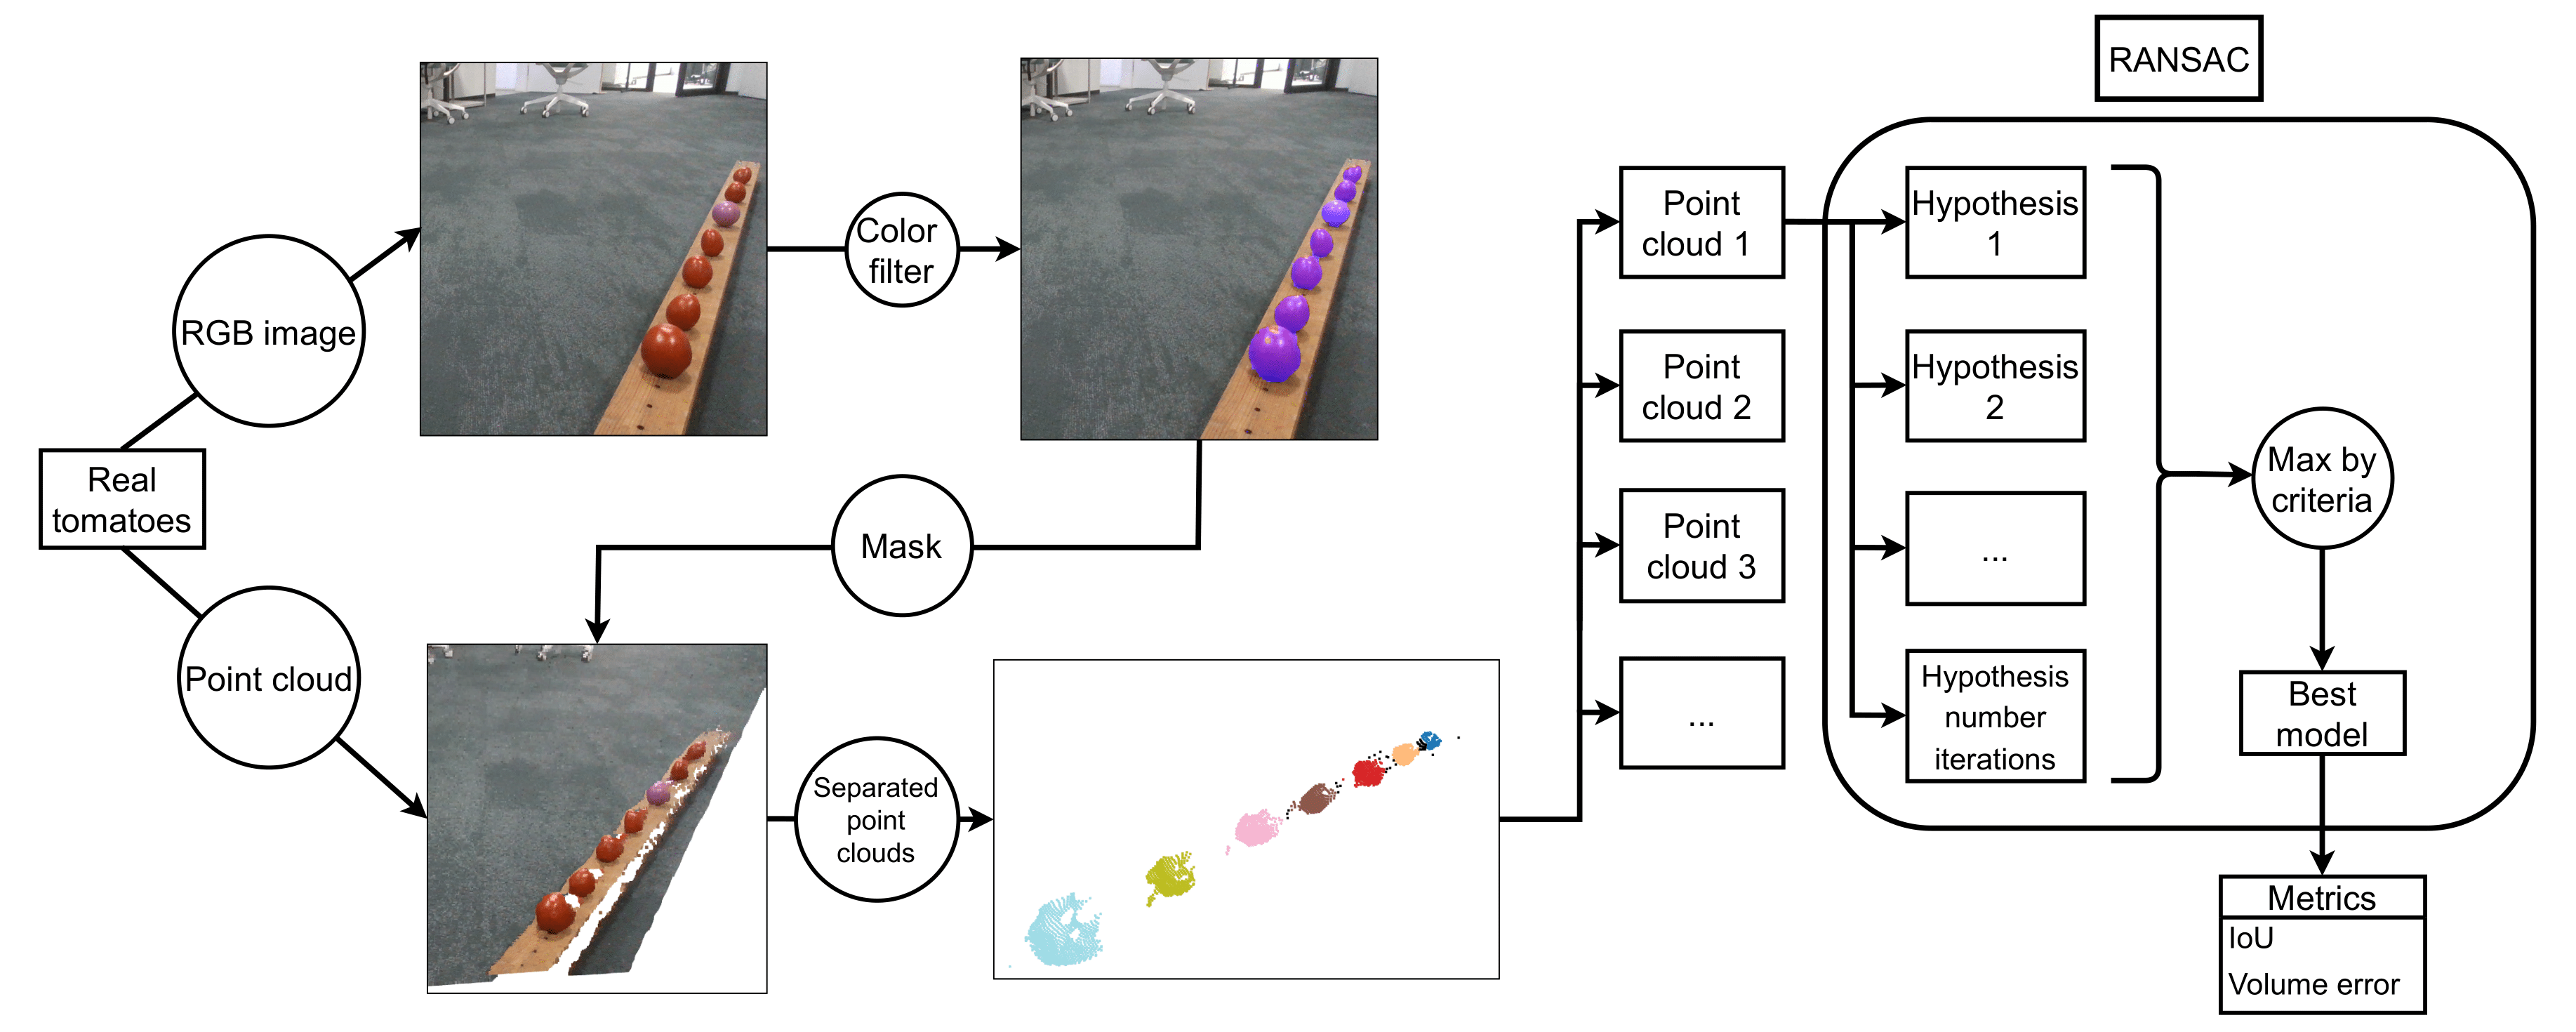
\includegraphics[width=0.98\textwidth]{gfx/DIAG.png}
      \caption{The scheme of the experimental setup. First, an RGB and depth-images are taken. Second, a color-based filter is applied to the RGB image and the corresponding parts of the point cloud are cut. Finally, RANSAC if applied to each of the objects and the results are evaluated against the markup.}
      \label{fig:algo}
  %\end{subfigure}
\end{figure*}

The proof will begin with an ellipse in the XY-plane and then be extended to the ellipsoid.

First, consider a set of points on the unit circle, $P_c$:

\begin{equation}
 P_c = \{ r_c \in \mathbb{R}^2 \ | \ r_c^Tr_c = 1\}. \tag{1}
\end{equation}

Let us introduce

\begin{align*}
  & t \in \mathbb{R}^2 \ - \ \text{translation vector,} \\ 
  & s \in \mathbb{R}^2 \ - \ \text{scale vector,} \\
  & \alpha \in [0, 2 \pi) \ - \ \text{rotation angle.} & \tag{2}
\end{align*}

With the matrix operations it is possible to transform unit circle into an arbitrary ellipse.

Let us unwrap the full form of these matrices.

\begin{align*}
  & S = \begin{pmatrix}
    s_1 & 0\\
    0 & s_2
  \end{pmatrix}
  \quad \parbox{0.28\textwidth}{ $-$ scale matrix, where $s_1$ and $s_2$ are parameters of scale vector $\textbf{s}$,} \\
  & R = \begin{pmatrix}
    \cos(\alpha) & -\sin(\alpha) \\
    \sin(\alpha) &  \cos(\alpha)
  \end{pmatrix}
  \quad \text{$-$ rotation matrix.} & \tag{3}
\end{align*}

Let $P_e$ be the points of the ellipse.
Scaling, rotation and translation of the unit circle yields

\begin{align}
 P_e = \{RSr_c + t \ |  r_c \in P_c\}. \tag{4}
\end{align}

From $(1)$ a matrix equation of the ellipse can be obtained.
For $r \in P_e$ the equation of the ellipse takes form of

\begin{align}
  & (r-t)^T [R^{-1}]^T [S^{-1}]^T  S^{-1}R^{-1}(r - t) = 1. \tag{5}
\end{align}

Since $R$ is an orthogonal matrix and $S$ is a diagonal matrix, $R^{-1} = R^T$ and $S^T = S$.

\begin{align}
  & (r^T - t^T) R S^{-2} R^T (r -t) = 1. \tag{6}
\end{align}

Let us introduce $V = R S^{-2} R^T$ for convenience.
Inserting this into equation $(6)$ yields:

\begin{align}
  & r^T V r - 2t^T V r + t^T V t = 1. \tag{7}
\end{align}

Let us also introduce vector $v^T = t^T V$ and scalar $v_0 = t^TVt$.

\begin{align}
  & r^T \bigg[\frac{V}{v_0-1}\bigg] r - 2 \bigg[\frac{v^T}{v_0-1} \bigg] r + 1 = 0. \tag{8}
\end{align}

Finally, let us define a matrix $M = \frac{V}{v_0-1}$ and a vector $m^T = \frac{v^T}{v_0-1}$.
Now it is possible to formulate the general matrix equation of an ellipse as follows:

\begin{align}
  r^T M r - 2 m^T r + 1 = 0.
\tag{9}
\end{align}

From this equation all the parameters needed to describe an arbitrary $n$-dimensional ellipsoid can be extracted, specifically translation, rotation and scaling.

Let us evaluate $M^{-1}$ first.

\begin{align}
M^{-1} = \bigg[\frac{V}{v_0-1}\bigg]^{-1} = (v_0-1)V^{-1} = (v_0-1)RS^2R^T.
\tag{10}
\end{align}

It could be observed that

\begin{align}
 t = M^{-1}m.
\tag{11}
\end{align}

Considering the eigendecomposition of $M$ yields

\begin{align*}
  M = \frac{1}{v_0-1} V = \frac{1}{v_0-1} R S^{-2} R^T = \\
  R\bigg[\frac{1}{v_0-1} S^{-2} \bigg] R^T = Q \Lambda Q^{-1}.
\tag{12}
\end{align*}

From $(12)$ it could be seen that the eigenvectors matrix of $M$ is exactly the rotation matrix $R$.

\begin{align}
  R = Q.
\tag{13}
\end{align}

Moreover, the matrix of the eigenvalues $M$ and $S$ are diagonal matrices:

\begin{align}
  \Lambda  = \frac{1}{v_0-1} S^{-2}.
  \tag{14}
\end{align}

Thus, it becomes possible to extract the scale matrix $S$ from the eigenvalues matrix $\Lambda$.

Scale matrix $S$ consists of squeezes and stretches along orthogonal axes of the ellipse, or just radii. Each eigenvalue can be presented as

\begin{align}
  \lambda_i  = \frac{1}{v_0-1} s_i^{-2}.
\tag{15}
\end{align}

In order to extract the radii, it is necessary to find $v_0$ first.
Since

\begin{align}
   v^TV^{-1}v & = v_0.
\tag{16}
\end{align}

And

\begin{align}
   m^TM^{-1}m = \frac{1}{v_0-1} v_0.
\tag{17}
\end{align}

Finally, an expression for $s_i$ can be found.

\begin{align}
   s_i = \sqrt{\frac{m^TM^{-1}m - 1}{\lambda_i}}.
\tag{18}
\end{align}

%For practical convinience we used a bit different coeficients in matrices definition, but the main point remained the same.
The solution holds with respect to the permutations of the axes of the ellipse.

\section{Data}
\label{sec_data}

Three sets of data were used in the numerical experiments.
The first are the synthetic ellipsoids generated with a naive straightforward method, see subsection \ref{subsec_ray_data}.
The second are the data generated with the ray emulation approach, see subsection \ref{subsec_naive_data}.
Finally, the third is the real data recorded with Intel RealSense D435i camera, see subsection \ref{subsec_real_data}.
Let us describe these sets of data.

\subsection{Naive synthetic ellipsoids generation}
\label{subsec_naive_data}

The first dataset contains points evenly distributed on the surface of ideal ellipsoids.
The ellipsoid is described by its center, semiaxes, and rotation.
After specifying those, a point cloud is created, consisting of points on the surface of the ellipsoid.
These data were used as the simplest possible to evaluate the algorithm's performance.
As one might expect, the error on clear data was precisely zero, so data with additive normal noise was considered as well, see Table \ref{tabularx:iou_tables} and Table \ref{tab:vol_table}.

The point clouds that are generated this way are different from the real ones due to the non-uniform surface coverage in the real data and only partial visibility to the real camera.

\subsection{Ray emulation-based synthetic data generation}
\label{subsec_ray_data}

Thus, an alternative approach was taken with a proper geometrical model of the camera.
Stereoscopic vision, either active or passive, relies on the difference in the appearance of the same objects from two distinct viewpoints.
Their correspondence allows for the reconstruction of the depth in the scene.
It should be noted that with such an approach the ellipsoid is covered with points not uniformly, see Figure \ref{fig_tomatoes_projection}.
An explicit geometrical model was used to obtain data that closely resembles the real point clouds.

\label{ell_line_int}
According to the used model, a tomato can be represented as an ellipsoid. 
Hence, the point cloud obtained from a real tomato can be approximated as the point cloud of an ideal ellipsoid. 
In this section, the process of image formation is considered. \\

\begin{figure}[!htb]
  \centering
  %\begin{subfigure}{0.48\textwidth}
  %    \centering
      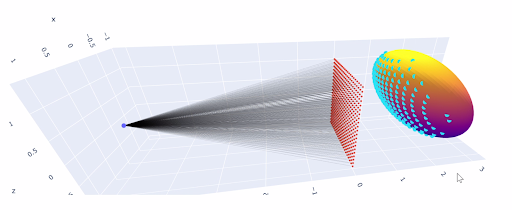
\includegraphics[width=0.48\textwidth]{gfx/images/synthetic_data/tomato.png}
      \caption{Scheme of the ray tracing-based approach to point cloud generation. On the left a focus of the camera is presented, the red grid in the middle is the camera matrix, and the rays casted from through it intersect with the surface of the ellipsoid in the points marked with cyan triangles.}
      \label{fig_tomatoes_projection}
  %\end{subfigure}
\end{figure}

The leftmost violet point in Figure \ref{fig_tomatoes_projection} represents the focal center of the camera, while the red points correspond to the light-sensitive pixels of the camera matrix. 
A line between the blue and red points visualizes a beam of light reflected from the ellipsoid that intersects with the camera matrix.
Extending this line to intersect with the ellipsoid yields a point in the point cloud (cyan triangles). 
%To create a more realistic point cloud, it is essential to introduce noise; however, for the purposes of this discussion, we will first consider the ideal scenario. 
Thus, the problem of finding the intersection of a line formed by two points with the ellipsoid needs to be addressed. \\

Let us consider an ellipsoid defined by $S$ (scale matrix), $R$ (rotation matrix), and $t$ (translation vector), 
along with a line formed by points $A$ and $B$. \\

First, let us transform the ellipsoid so that it becomes a unit sphere at the origin in order to simplify the problem.
The points $A$ and $B$ will be transformed as follows:

\begin{align*}
A' &= S^{-1} R^T (A - t), \\
B' &= S^{-1} R^T (B - t).
\tag{19}
\end{align*}

The direction vector defining the light beam line in the new coordinates can be found as:

\begin{align*}
a &= \frac{A' - B'}{\|A' - B'\|}.
\tag{20}
\end{align*}

The solution for the line-sphere intersection yields two points $P_1$ and $P_2$, that can be found according to the subsequent computational steps derived from solving a quadratic equation, if $\Delta \geq 0$.

\begin{align*}
\Delta & = (a^T A')^2 - (A')^T A  + 1, \\
C' & = A' - a^T A' a, \\
P_1' & = C' - a \sqrt{\Delta}, \\
P_2' & = C' + a \sqrt{\Delta}, \\
P_1 & =  R S (P_1' + t), \\
P_2 & =  R S (P_2' + t). \\
\tag{21}
\end{align*}

By repeating this algorithm for each red point representing pixels, an array of points that lie on the ellipsoid is formed, see Figure \ref{fig:synth_segment_clean}.
After that the noise is added into the data, see Figure \ref{fig:synth_segment_noise}.
The amplitude of noise was chosen in accordance with the real data.

\begin{figure}
  \centering

  \begin{subfigure}[b]{0.42\textwidth}
      \centering
      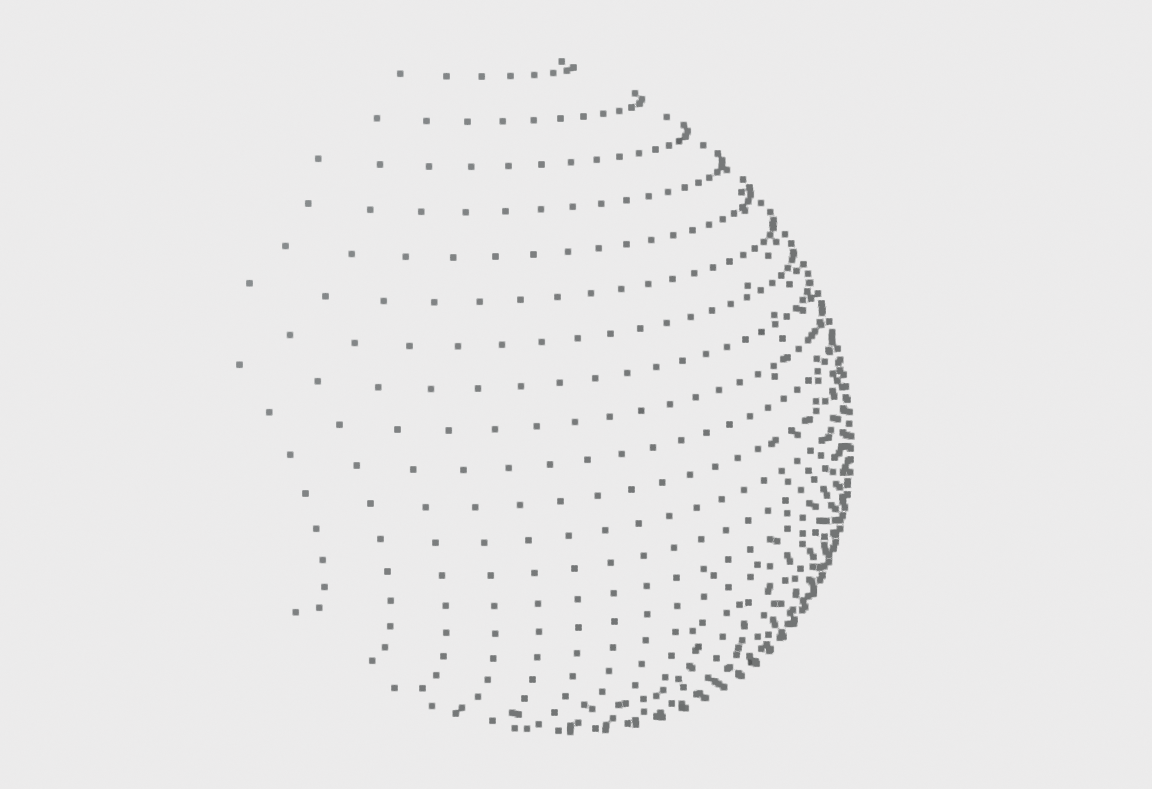
\includegraphics[width=\textwidth]{gfx/images/datasets/segment_image_without_noise.png}
      \caption{Example of a point cloud of an ellipsoid segment without noise}
      \label{fig:synth_segment_clean}
  \end{subfigure}
  \hfill
  \begin{subfigure}[b]{0.42\textwidth}
      \centering
      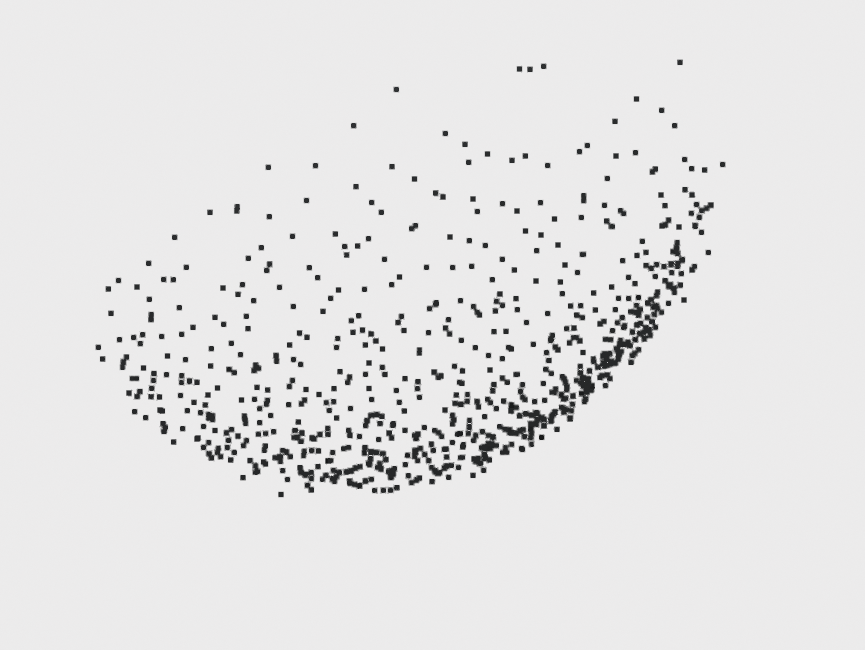
\includegraphics[width=\textwidth]{gfx/images/datasets/segment_image_with_noise.png}
      \caption{Example of a point cloud of an ellipsoid segment with noise}
      \label{fig:synth_segment_noise}
  \end{subfigure}
  \caption{Samples from a part of the synthetic dataset, generated with the ray tracing: (a) clear (b) with additive normal noise.}
  %\label{fig_segments}
\end{figure}

%The last stage of working with synthetic data was testing the algorithm on ellipsoid segments, to which normal noise was added.
%This brought the data closer to real shooting conditions, when the depth camera captures only a limited part of the object with the presence of noise caused by imperfect equipment and shooting conditions \ref{fig:synth_segment_noise}.

%For each data set, the parameters of the generation and point cloud were saved, both with and without noise, which made it possible to conduct a comparative analysis of the algorithm's operation in different conditions.

\subsection{Real data}
\label{subsec_real_data}

%\subsubsection{Tomatoes on a horizontal plane}\label{sec:ch3/sec3/subsec2/subsubsec1}

\begin{figure}[!htb]
  \centering
  %\begin{subfigure}{0.48\textwidth}
  %    \centering
      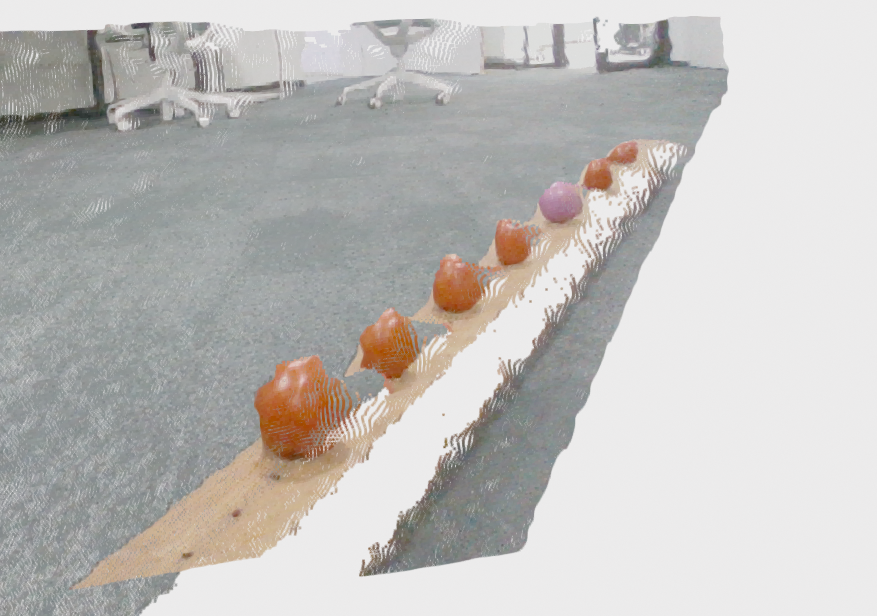
\includegraphics[width=0.48\textwidth]{gfx/images/datasets/wood_data.png}
      \caption{Sample point cloud from the real part of the dataset. Tomatoes and a rubber ball are placed on a wooden support.}
      \label{fig:wood_data}
  %\end{subfigure}
\end{figure}

The point cloud in the Figure \ref{fig:wood_data} is from the real part of the dataset.
These point clouds are a challenging piece of data.
Tomatoes are described by an ellipsoid model only in a certain approximation, varying from fruit to fruit and from strain to strain.
It means that even the best possible fit will result in a certain non-zero error.

Moreover, the real noise cannot be approximated by the normal noise model.
In the Figure \ref{fig:hist_for_segment_distances} the distribution of the algebraic distance from the ellipsoid surface is presented for the synthetic data.
In the Figure \ref{fig:wood_rs_55_pcds_distances_over_real_hist_plot_wood} the same is given for the real data.
It could be seen that the distribution for the real data is not unimodal and skewed for all three tomatoes considered, meaning that the real data does not fully comply with the used model.

The last considerable obstacle are the distortions that occur on the surface of the tomatoes.
The exact reasons behind this effect are not clear, but such a distorted appearance was noticed a number of times.

%\blue{
The ways to deal with these complications include the following.
In order to account for the tomatoes being not precisely ellipsoid a more general model of the fruit can be used, such as hyperellipsoids or even the most general case, such as a combination of shperical harmonics.
The noise with the complex distributions can be dealt with by standard RANCAS, as numerical experiments on the real data suggest.
Finally, end-to-end algorithms, such as neural networks, can be used.
%}

To test the algorithm on real data, a series of experiments was conducted with tomatoes located on a horizontal wooden board.
The experiment involved six tomatoes and one rubber ball, that were placed at a distance of between 10 and 15 \si{cm} from each other, see Figure \ref{fig:wood_data}.
The camera captured scenes at various angles of the board: 55, 60, 70, 80 and 90 degrees.
This made it possible to study the effect of the viewing angle on the perception of the shape of objects by the depth camera.
For each angle, 146 point clouds were taken.
Each point cloud contains approximately 111,000 points, where nearly 2,200 belong to the tomatoes.
For a single object this number varies from 831 points for the nearest one to 130 for the farthest.
The volume of the tomatoes ranges from 90 to 207 cubic \si{cm}.
For each tomato the ball their actual size and volume were measured, and the exact location relative to the camera was determined.
In this experiment, tomatoes were modeled as ideal spheres, where the radius of the sphere was determined by the average value of the semi-axes of the ellipsoid.
The tomatoes used were reasonably close to a sphere, which made it possible to make this assumption fair.
As a result, a dataset was created containing the centers and radii of objects, that were compared with the output of the algorithm.

\begin{figure}[!htb]
  \centering
      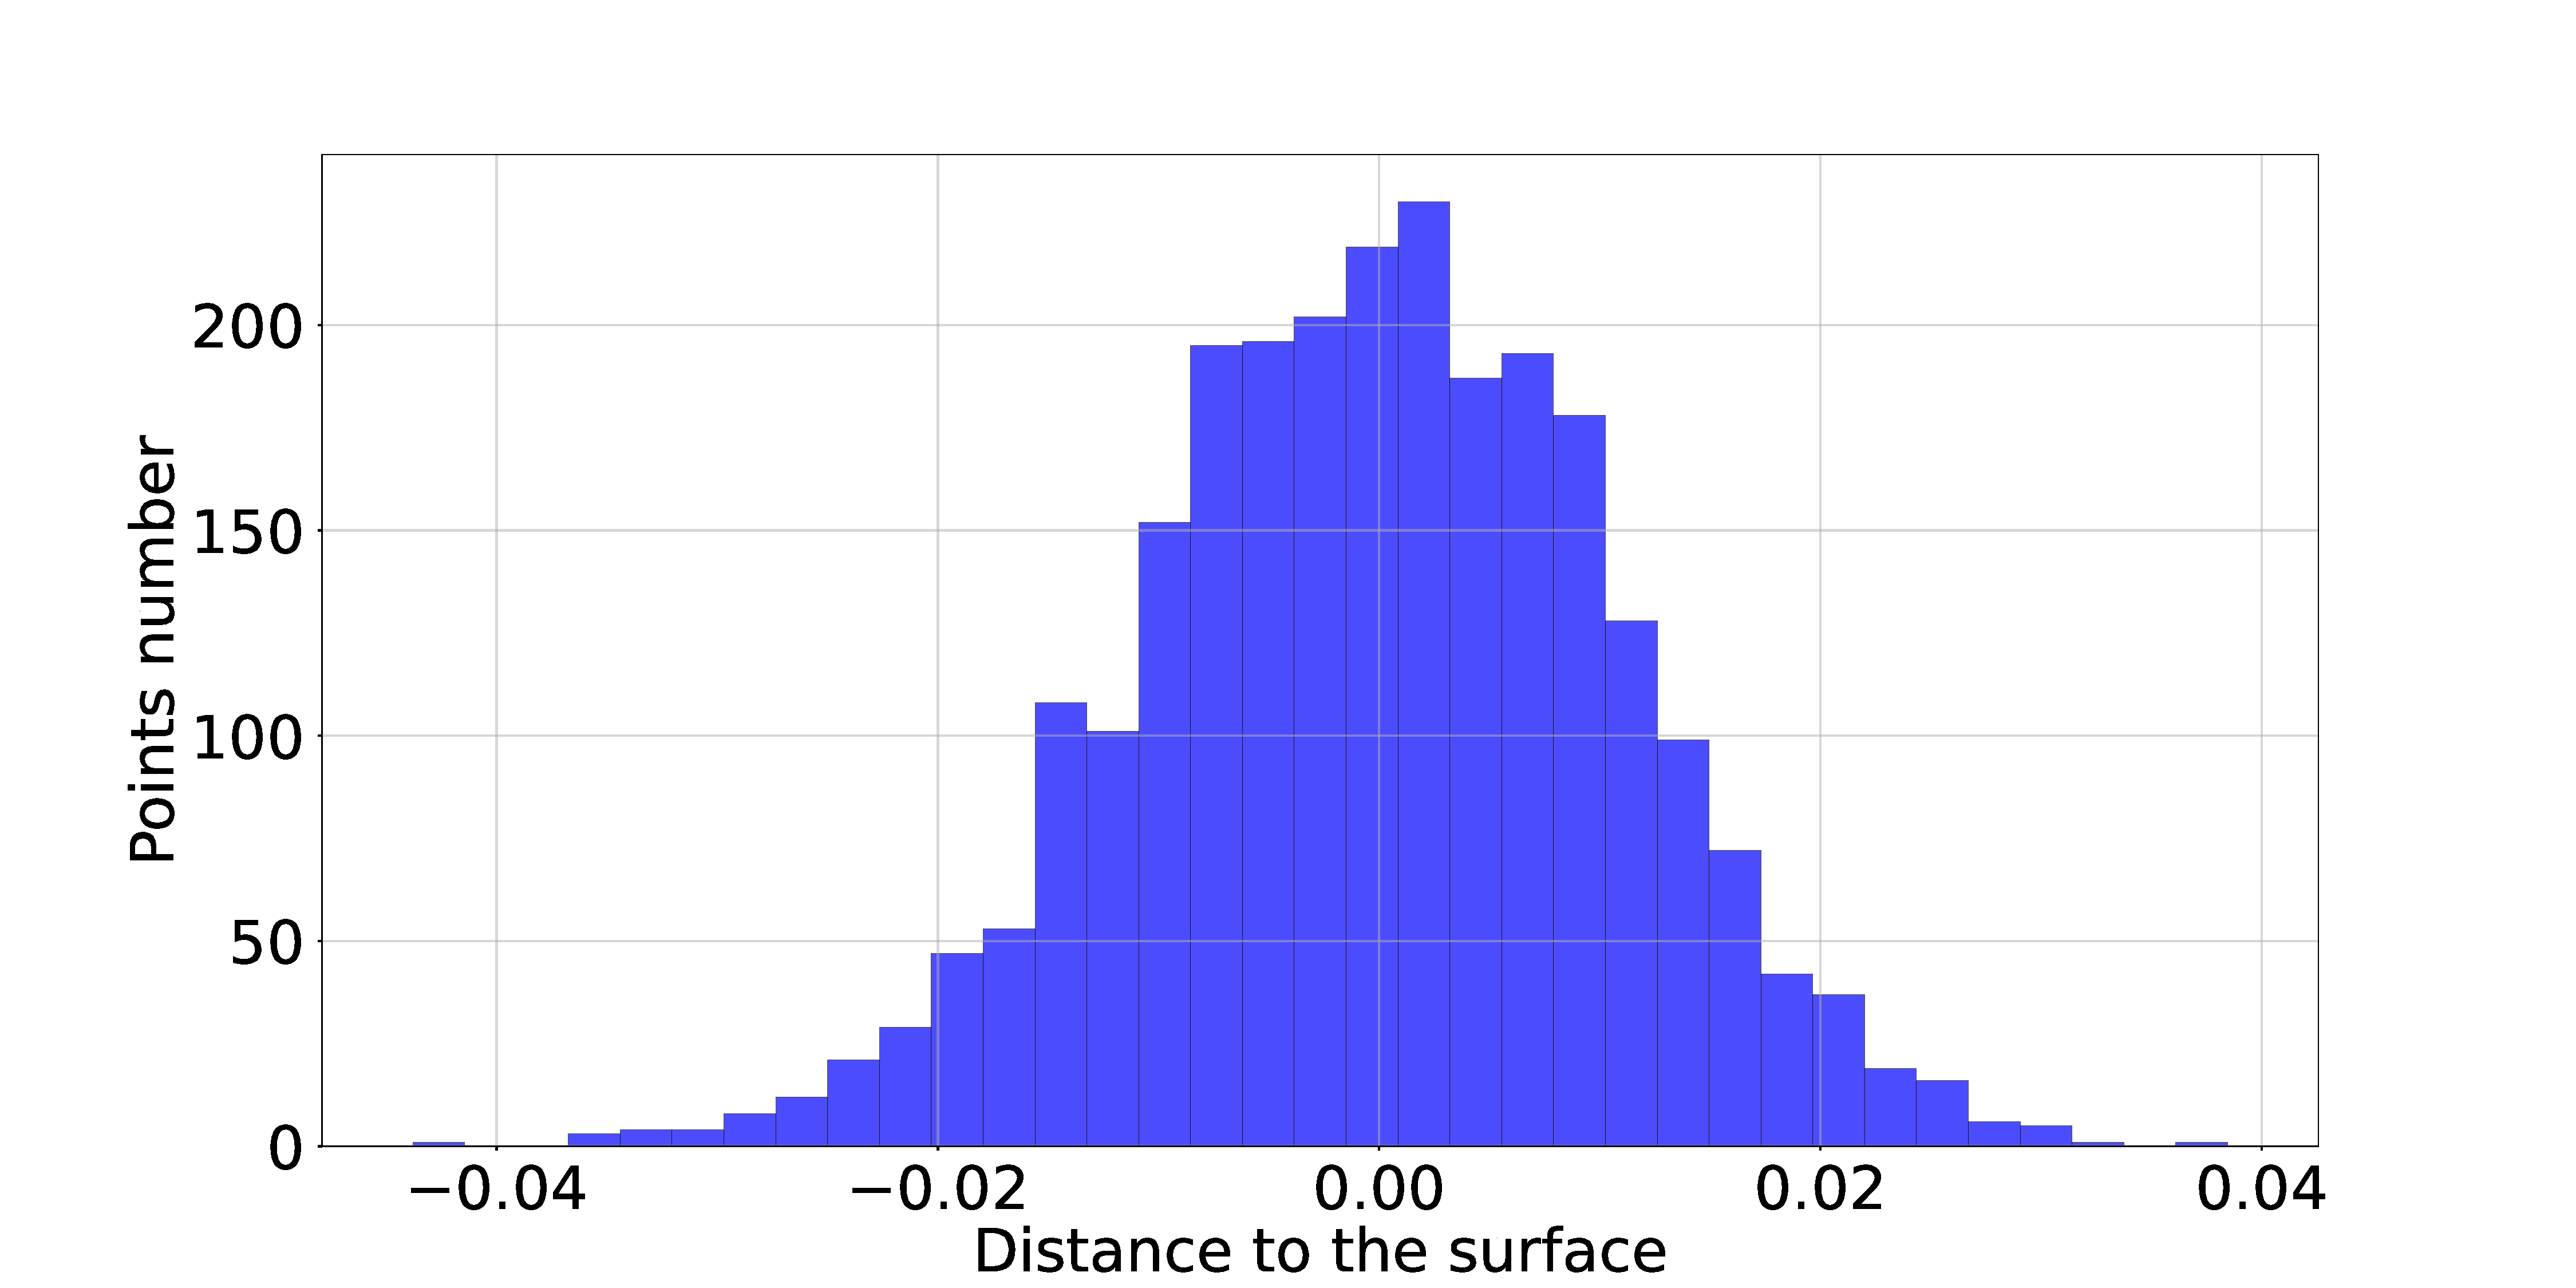
\includegraphics[width=0.48\textwidth]{images/wood_synth_distances_over_real_hist_plot_wood.pdf}
      \caption{Distribution of the algebraic distance between the points and the surface of the best fitted ellipsoid model for synthetic data. A clear unimodal distribution can be seen.}
      \label{fig:hist_for_segment_distances}
\end{figure}

\begin{figure}[!htb]
  \centering
  %\begin{subfigure}{0.48\textwidth}
  %    \centering
      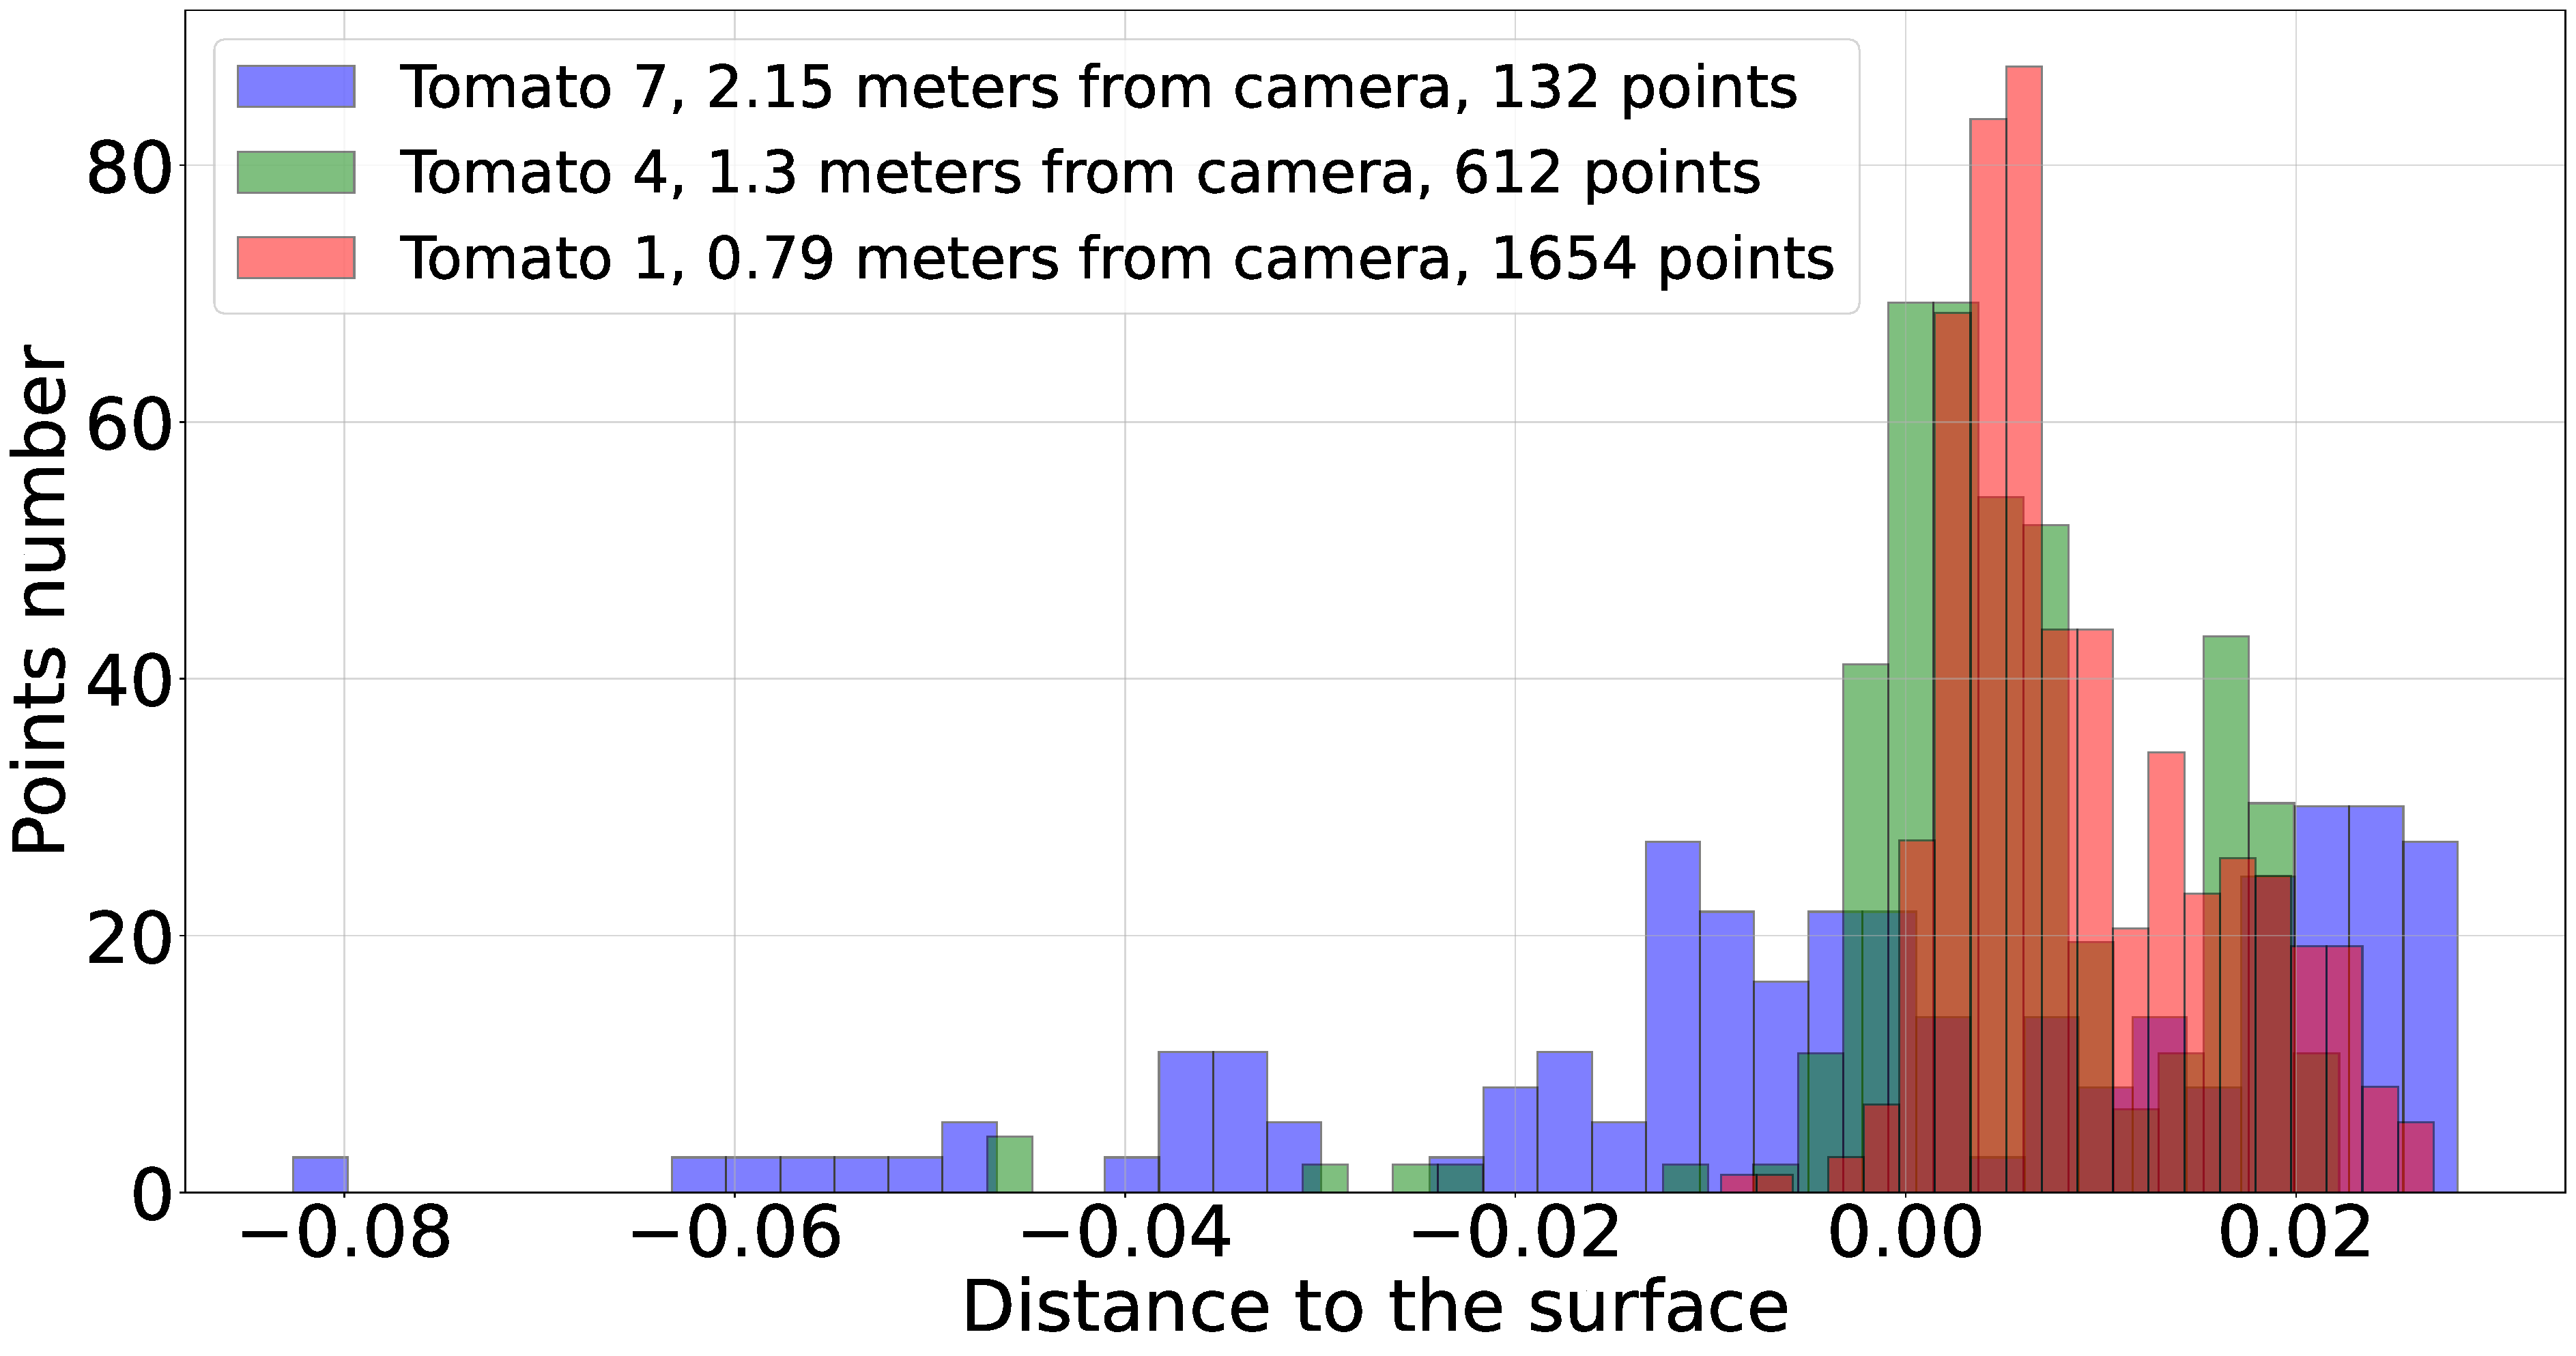
\includegraphics[width=0.48\textwidth]{images/wood_rs-55_pcds_distances_over_real_hist_plot_wood2}
      \caption{Distribution of the algebraic distance between the points and the surface of the best fitted ellipsoid model for three tomatoes from the real data. For all three of them the distribution is rather noisy and clearly not unimodal, suggesting that the real data is significantly more challenging than synthetic.}
      \label{fig:wood_rs_55_pcds_distances_over_real_hist_plot_wood}
  %\end{subfigure}
\end{figure}

The real data was captured with Intel RealSense D435i.
The exposure and white balance were set to auto.
The scene was captured under artificial lighting.

\begin{table*}[!htb]
  \centering
  \begin{tabular}{lrrrrrrrr}
  \toprule
  \multirow{2}{*}{Iterations} & \multicolumn{4}{c}{Full ellipsoids with noise} & \multicolumn{4}{c}{Ellipsoid segments with noise} \\
  \cmidrule(lr){2-5} \cmidrule(lr){6-9}
   & 0.0 & 0.01 & 0.26 & 0.41 & 0.0 & 0.01 & 0.03 & 0.05 \\
  \midrule
  10 & 1.0 & 0.9518 & 0.5428 & 0.5238 & 0.9978 & 0.2403 & 0.1582 & 0.1022 \\
  100 & 1.0 & 0.9523 & 0.5714 & 0.5569 & 0.9989 & 0.3079 & 0.1555 & 0.0969 \\
  1000 & 1.0 & 0.9427 & 0.5497 & 0.5219 & 0.9995 & 0.3885 & 0.2086 & 0.1333 \\
  \bottomrule
  \end{tabular}
  \caption{Average IoU with different number of iteration (10, 100 and 1000) on different data: full noised ellipsoids and noised ellipsoid segments, generated with ray tracing}
  \label{tabularx:iou_tables}
  \end{table*}

\begin{table*}[!htb]
  \centering
  \begin{tabular}{lrrrrrrrr}
  \toprule
  \multirow{2}{*}{Iterations} & \multicolumn{4}{c}{Full ellipsoids with noise} & \multicolumn{4}{c}{Ellipsoid segments with noise} \\
  \cmidrule(lr){2-5} \cmidrule(lr){6-9}
    & 0.0 & 0.01 & 0.26 & 0.31 & 0.0 & 0.01 & 0.03 & 0.05 \\
  \midrule
  10 & 0.0 & 0.0071 & 0.5214 & 0.7591 & 0.0008 & 0.2173 & 0.6498 & 0.6690 \\
  5000 & 0.0 & 0.0267 & 0.5527 & 0.1307 & 0.0 & 0.1394 & 1.7770 & 0.5463 \\
  10000 & 0.0 & 0.0091 & 0.0742 & 0.0336 & 0.0 & 0.1394 & 0.3276 & 0.4036 \\
  \bottomrule
  \end{tabular}
  \caption{Average Relative Volume Error with different number of iteration (10, 100 and 1000) on different data: full noised ellipsoids and noised ellipsoid segments, generated with ray tracing}
  \label{tab:vol_table}
  \end{table*}

\section{Results}
\label{sec_results}

\begin{table}[h]
  \centering
  \begin{tabular}{|c|c|c|}
      \hline
      \textbf{Iteration number} & \textbf{Precision} & \textbf{Recall} \\
      \hline
      1250  & 0.5346 & 0.8564 \\
      2500  & 0.5611 & 0.8445 \\
      5000  & 0.5697 & 0.8601 \\
      7500  & 0.5705 & 0.8623 \\
      10000 & 0.5798 & 0.8856 \\
      \hline
  \end{tabular}
  \caption{Precision and Recall values for inliers for different number of iterations.}
  \label{tab:precision_recall}
\end{table}

%\section{Experimental setup}
%\label{sec_results}

%\subsection{Metrics}
%\label{subsec_metrics}

The experiments with the real data were conducted in accordance with the scheme in the Figure \ref{fig:algo}: RANSAC for ellipsoids is applied after cutting a part of the point cloud that consists of the object only.

The metrics that were used to assess the method's performance are the following.
First, it is the Intersection-over-Union between the real ellipsoid and the output of the algorithm.
Second, it is the ratio between the predicted and real volume of the ellipsoid.
Finally, it is the relative error in volume for the whole set of ellipsoids:
\begin{align*}
  \dfrac{\sum V_{predicted} - \sum V_{real}}{\sum V_{real}}. \\
  \tag{22}
  \end{align*}

%\blue{
The hyperparameters used are the following:
\begin{itemize}
    \item Threshold for the algebraic distance is 0.001
    \item Maximal iterations number is 10000. The results for the other iteration numbers are presented in the tables below
    \item Maximal acceptable ratio between the biggest and the smallest semiaxis is 2 (used for filtering)
    \item Maximal ratio between the maximal semiaxis of the ellipsoid and the maximal distance between the data points is 5 (used for filtering)
\end{itemize}
%}

\begin{figure}[!htb]
  \centering
  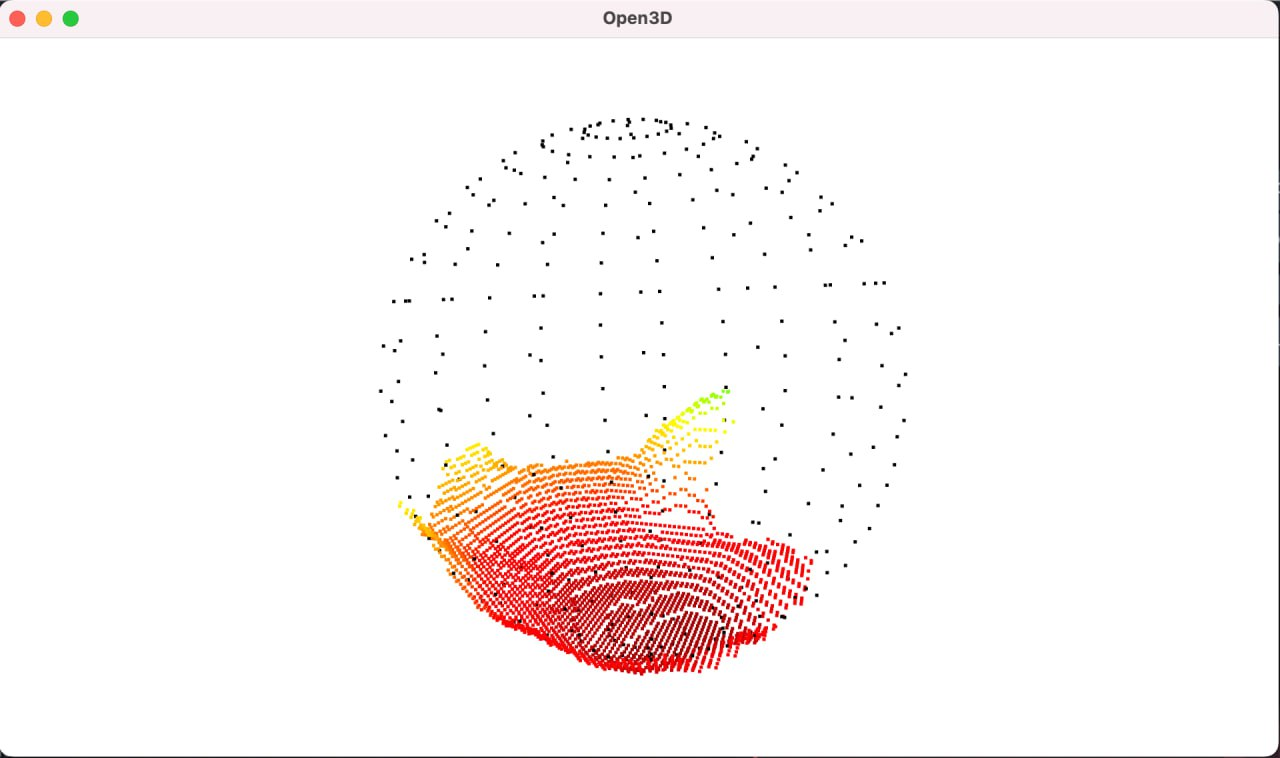
\includegraphics[width=0.48\textwidth]{images/ransac_synt2}
  \caption{Output of RANSAC on a point cloud from the real data. Notice that despite the complexity of the data, i.e. small section of the ellipsoid covered, non-uniform density, surface distortion — the output is reasonably good. This exact sample was cherry picked for demonstration purposes.}
\label{fig:real_data_output}
%\end{subfigure}
\end{figure}

\begin{figure}[!htb]
  \centering
  %\begin{subfigure}{0.48\textwidth}
  %    \centering
      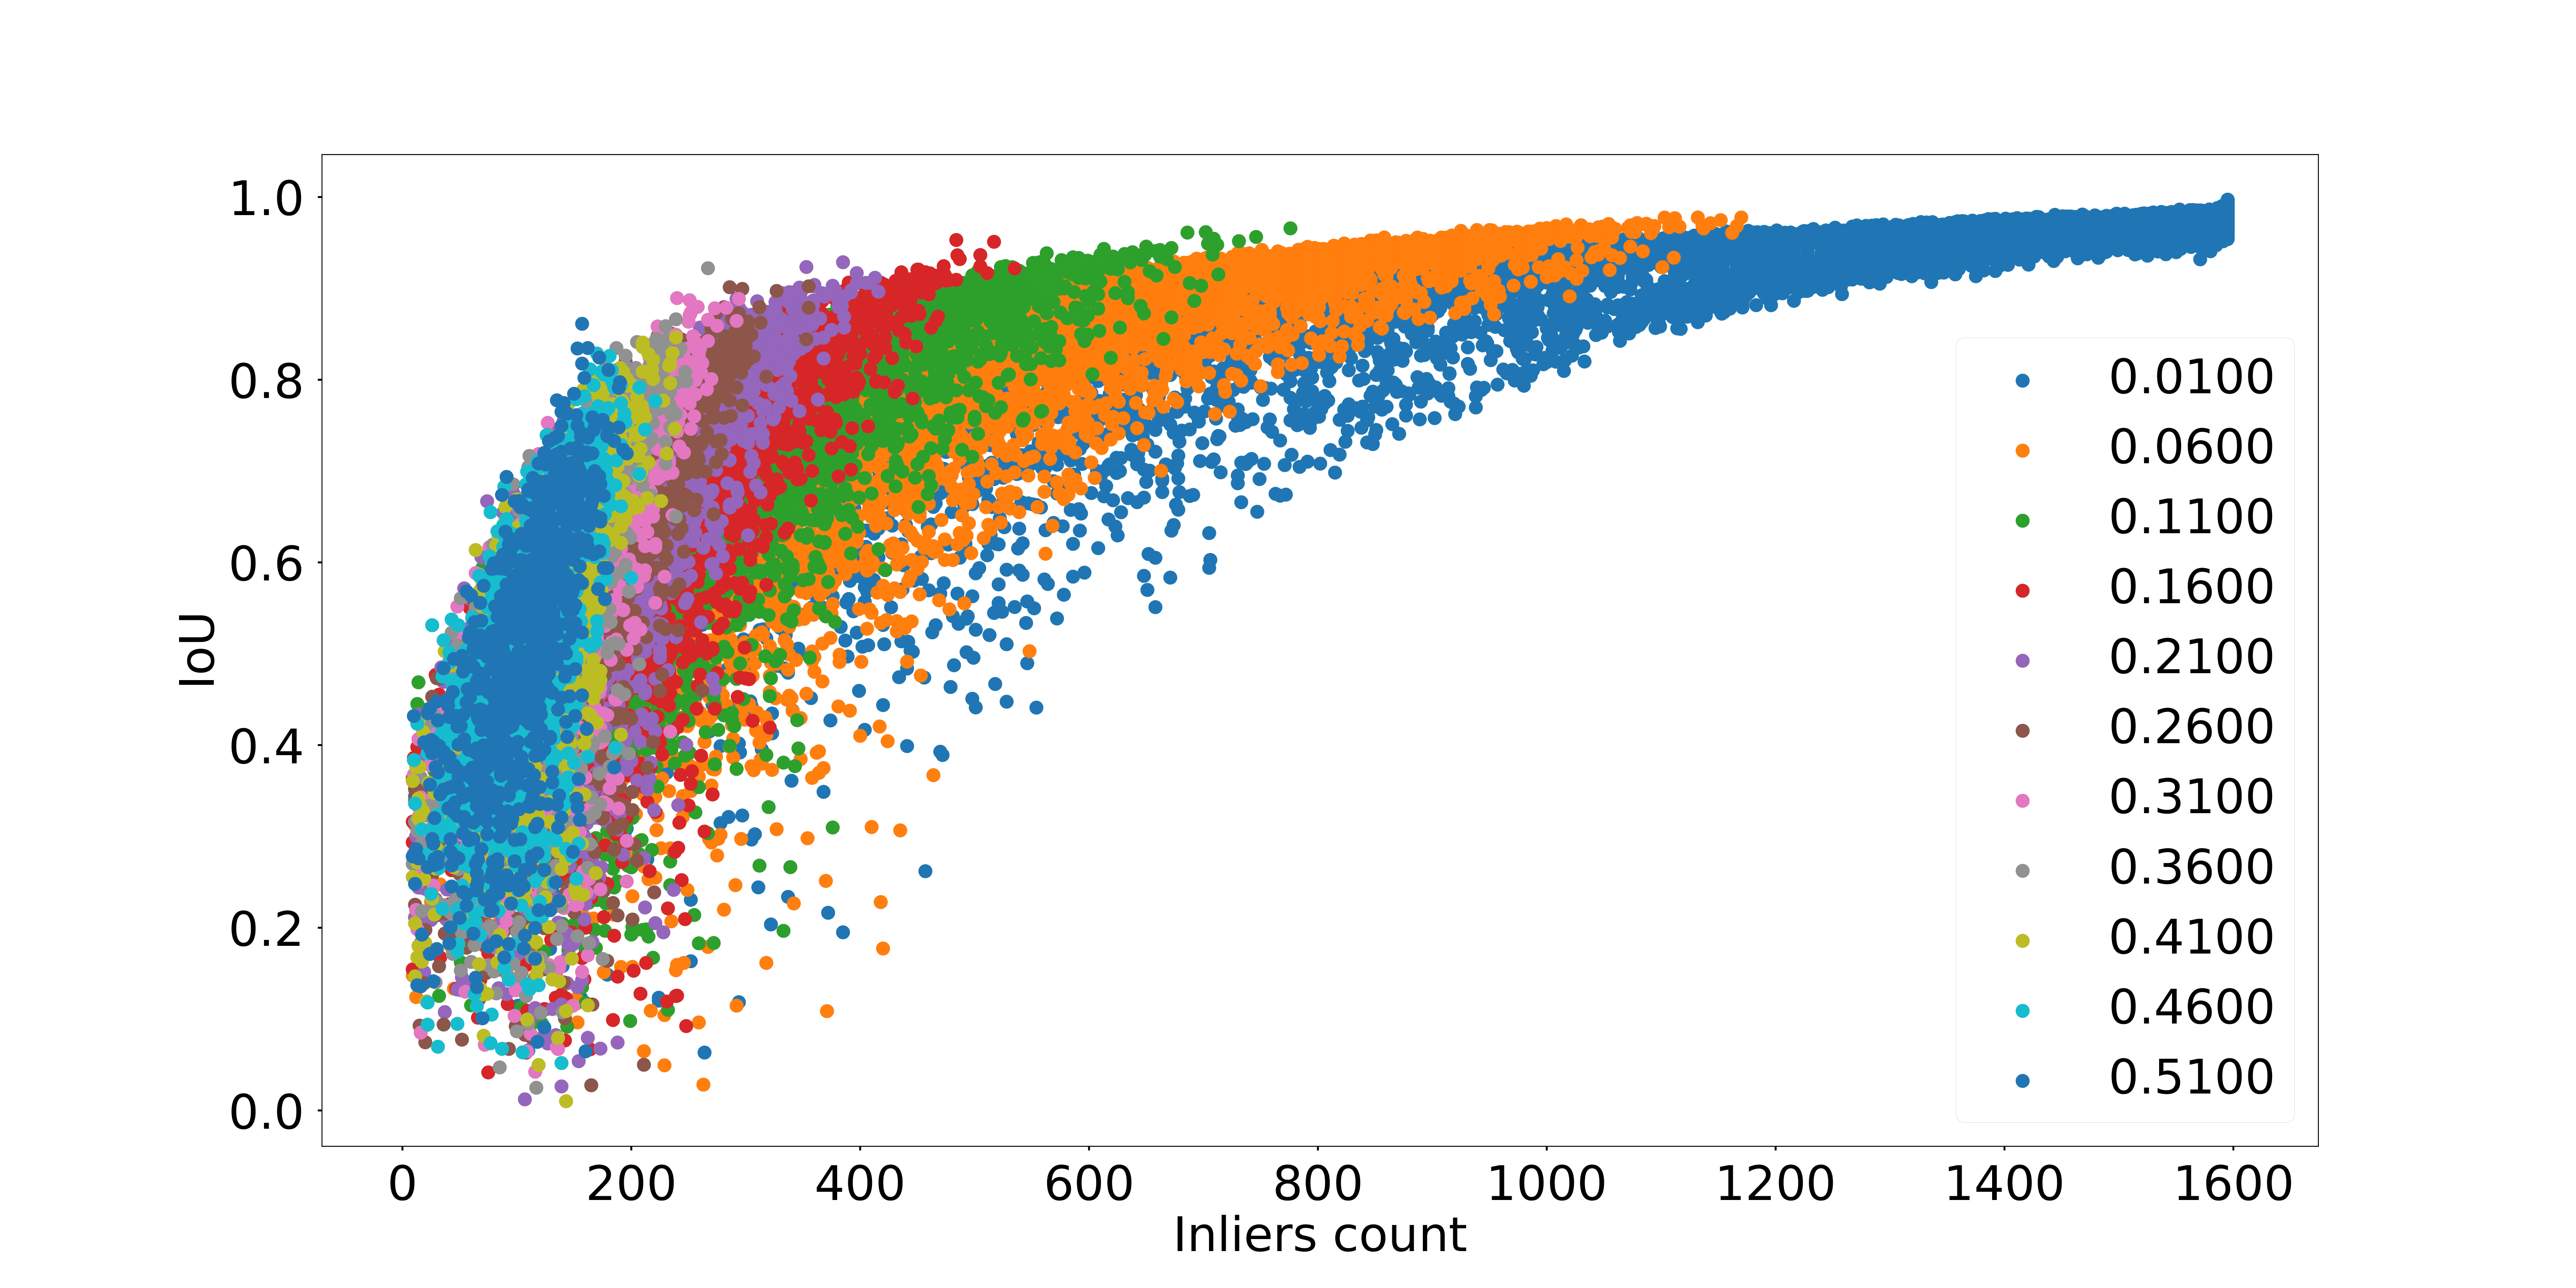
\includegraphics[width=0.48\textwidth]{images/iou_inlier_normal_noise.png}
      \caption{Mutual distribution of IoU and number of inliers for full ellipsoids with different noise amplitudes. A trend can be observed that generally the more inliers there are for the model, the higher the IoU with the true ellipsoid is.}
      \label{fig:iou_inlier_normal_noise}
  %\end{subfigure}
\end{figure}

Figure \ref{fig:iou_inlier_normal_noise} presents mutual distributions of a hypothesis IoU versus number of inliers for that model for different noise levels.
For very strong noise, the constellation of dots in the plot appears as an almost vertical blob.
It is bounded from the right, meaning that no model has lots of inliers.
Consequently, the influence of the stochastic nature of the algorithm can lead to unsatisfactory results.

On the other hand, with light noise a clear trend can be observed: with the growth of the number of inliers the quality in terms of IoU grows as well.
%Similar trend can be observed in terms or Relative Volume Error, see Figure \ref{fig:rve_inlier_normal_noise}.

\begin{figure}[!htb]
  \centering
  %\begin{subfigure}{0.48\textwidth}
  %    \centering
      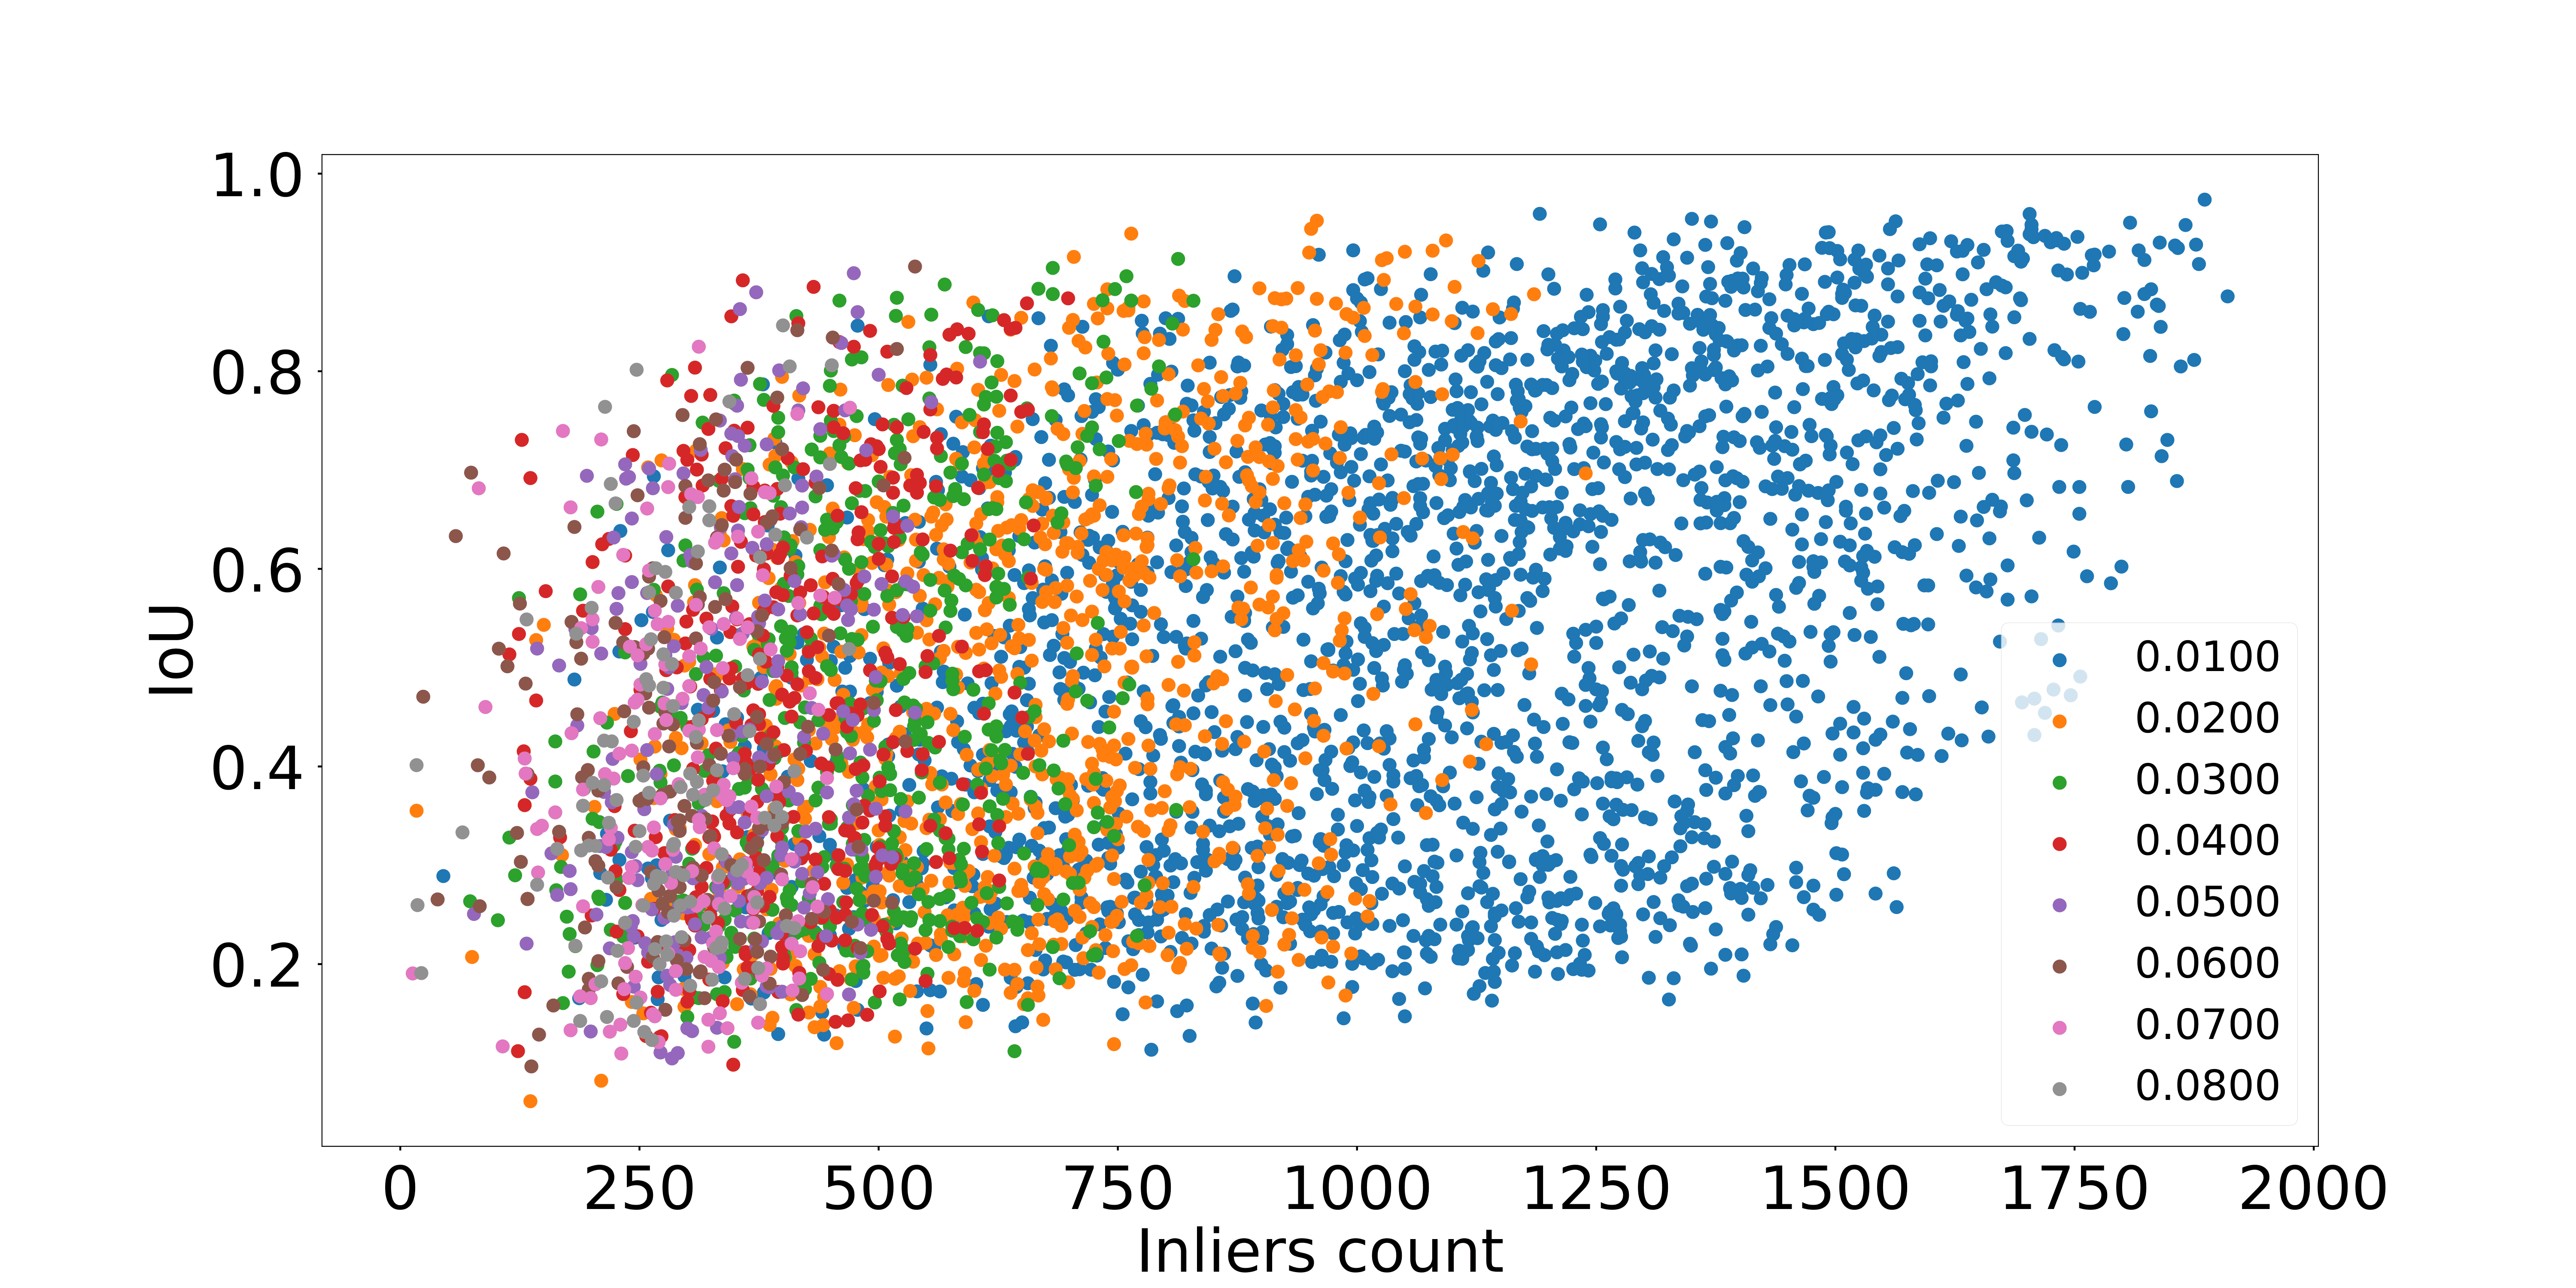
\includegraphics[width=0.48\textwidth]{images/iou_inlier_segment_normal_noise.png}
      %\caption{iou inlier segment normal noise 0.1}
      \caption{Mutual distribution of IoU and number of inliers for segments of ellipsoids with different noise amplitudes. In comparison with the Figure \ref{fig:iou_inlier_normal_noise} the trend is much less prominent.}
      \label{fig:iou_inlier_segment_normal_noise}
  %\end{subfigure}
\end{figure}

It could be noted that in the transition from the full ellipsoids to the segments, that are closer to the real data, the mutual distribution is blurred significantly, see Figure \ref{fig:iou_inlier_segment_normal_noise}.

\begin{figure}[!htb]
  \centering
  %\begin{subfigure}{0.48\textwidth}
  %    \centering
      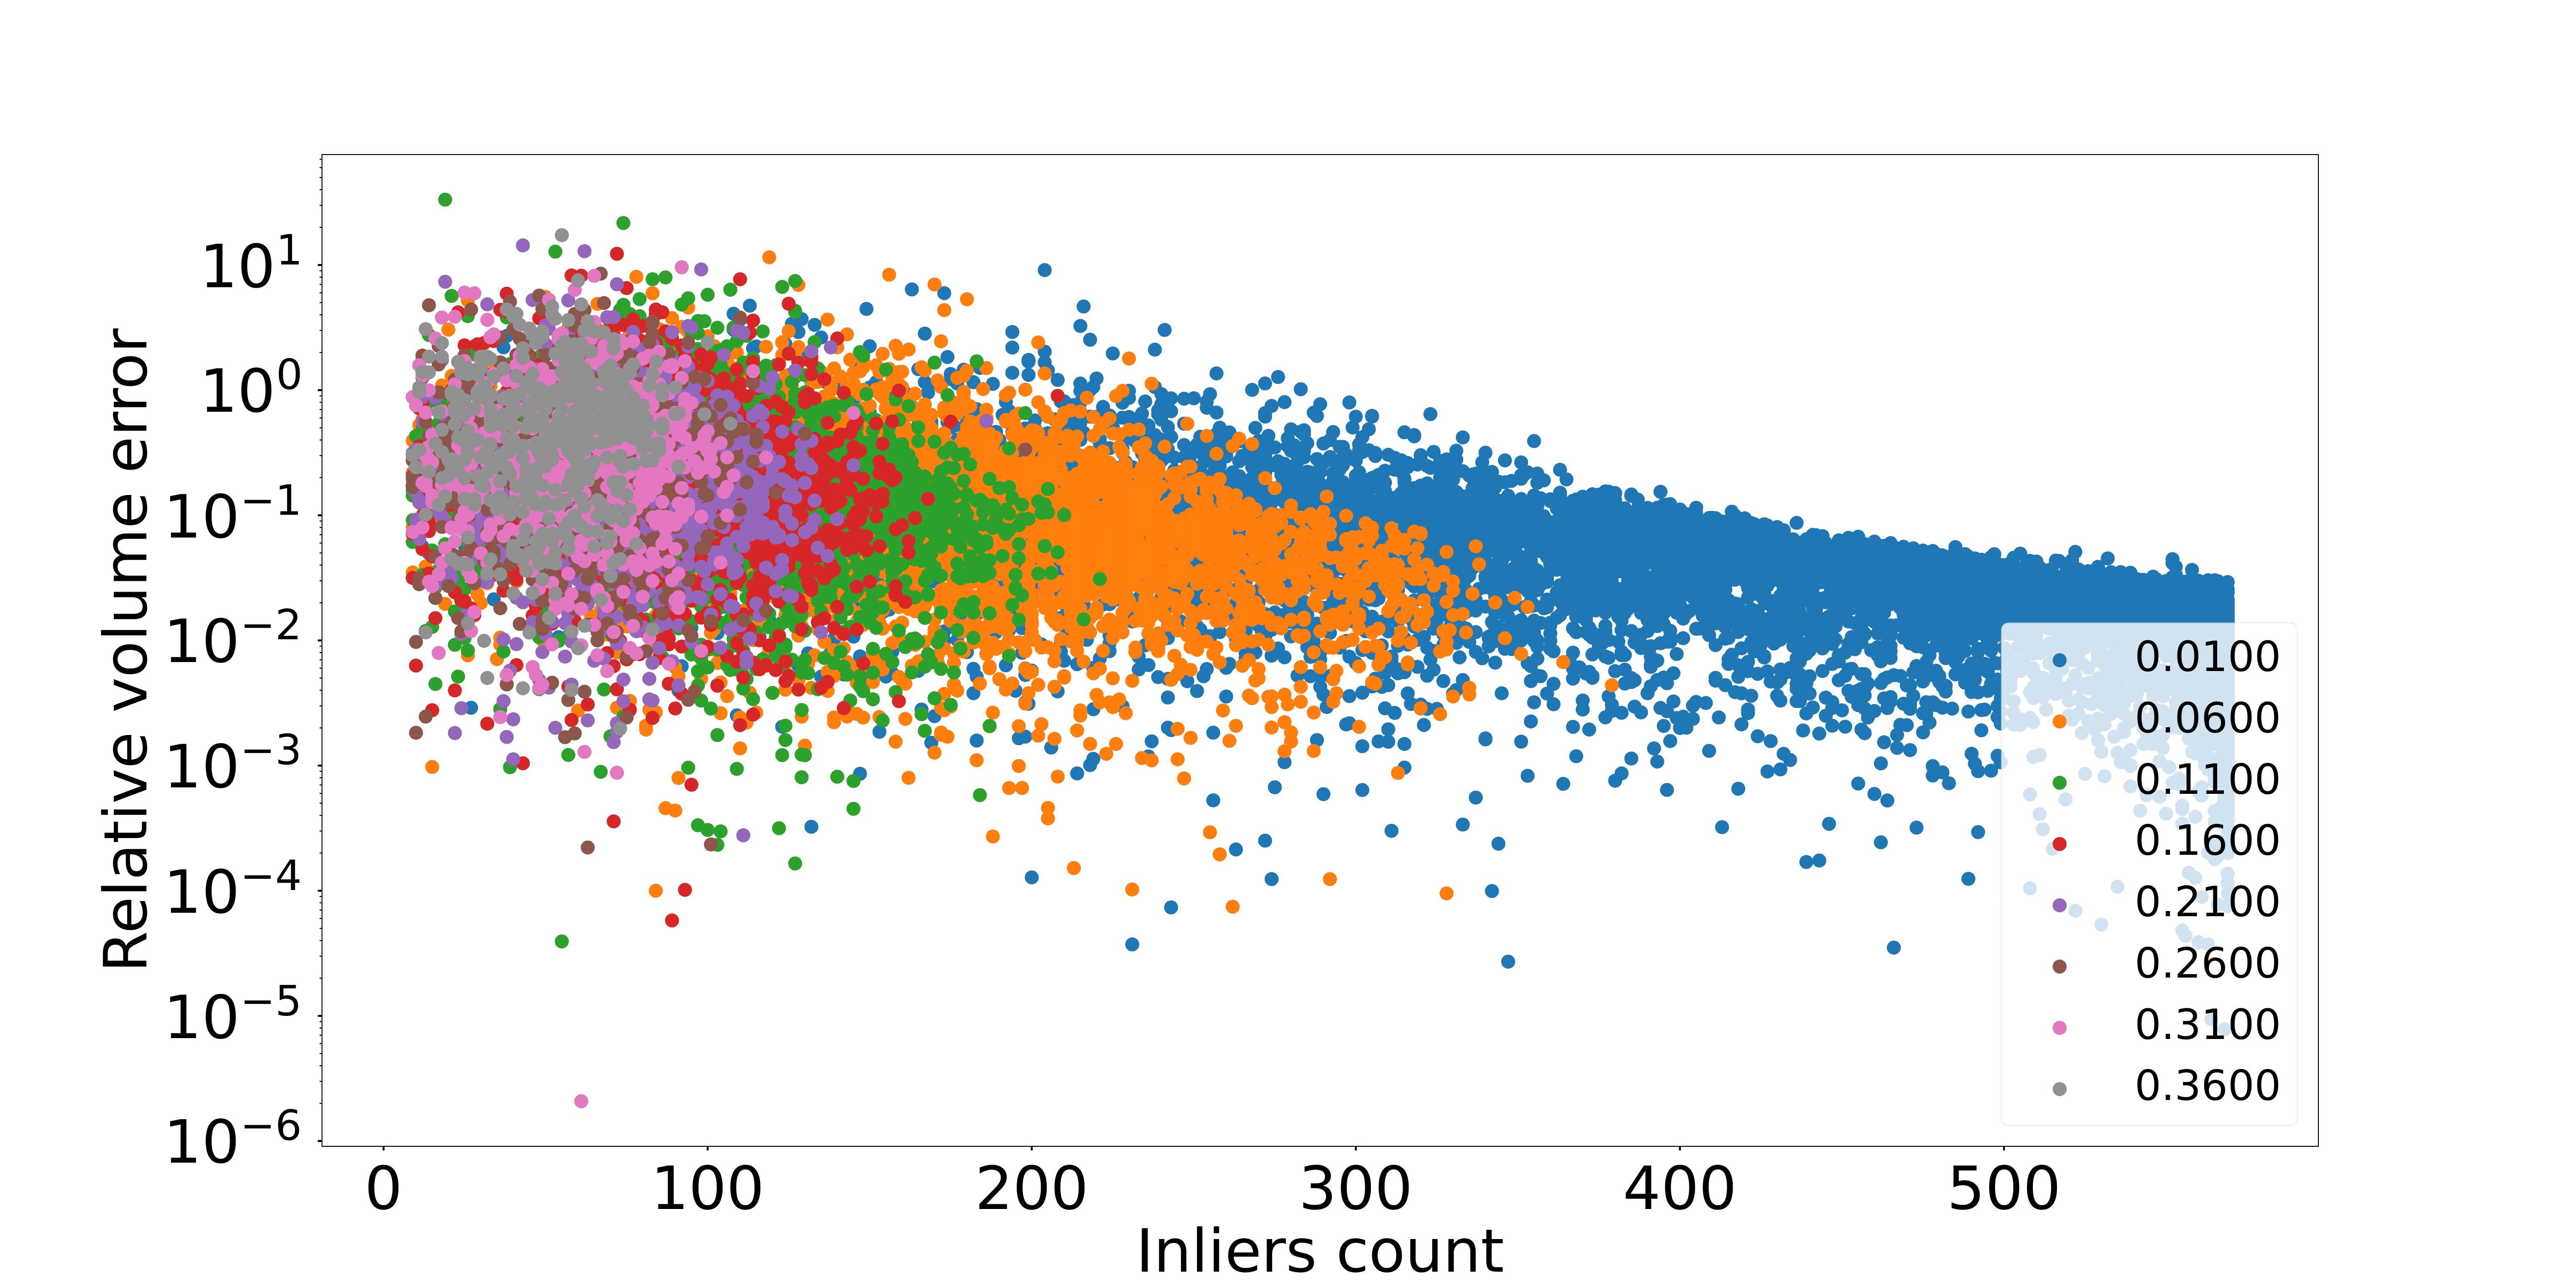
\includegraphics[width=0.48\textwidth]{images/rve_inlier_normal_noise.png}
      \caption{Mutual distribution of Relative Volume Error (RVE) and number of inliers for full ellipsoids with different noise amplitudes. With the growth of the number of inliers the average error declines.}
      \label{fig:rve_inlier_normal_noise}
  %\end{subfigure}
\end{figure}

Similar trend, but with the declining relative volume error can be observed on the Figure \ref{fig:rve_inlier_normal_noise}.
For strong noise the number of inliers is small and the overall volume error is high, and for the light noise it is the exact opposite.

It could be observed that there it a noisy, but distinct trend of the increase in the model quality with the increase of the inlier number.
However, due to the stochastic nature of the algorithm, it is not guaranteed that the best in terms of the IoU model will be the same that has the biggest inlier number.

%\blue{
Table \ref{tab:precision_recall} presents precision and recall for the inliers for the best fitted models.
An improvement in the quality can be observed as the number of iterations grows.
However, it is associated with a growing computtional burden, so a balance should be found for real applications between the quality of the output and the computational demands of the algorithm.
%}

Now let us observe the dependence of the quality of the best model as the number of algorithm iterations increase.

The results for the different number of iterations are presented in the Table \ref{tabularx:iou_tables}.

\begin{figure}[!htb]
  \centering
  %\begin{subfigure}{0.48\textwidth}
  %    \centering
      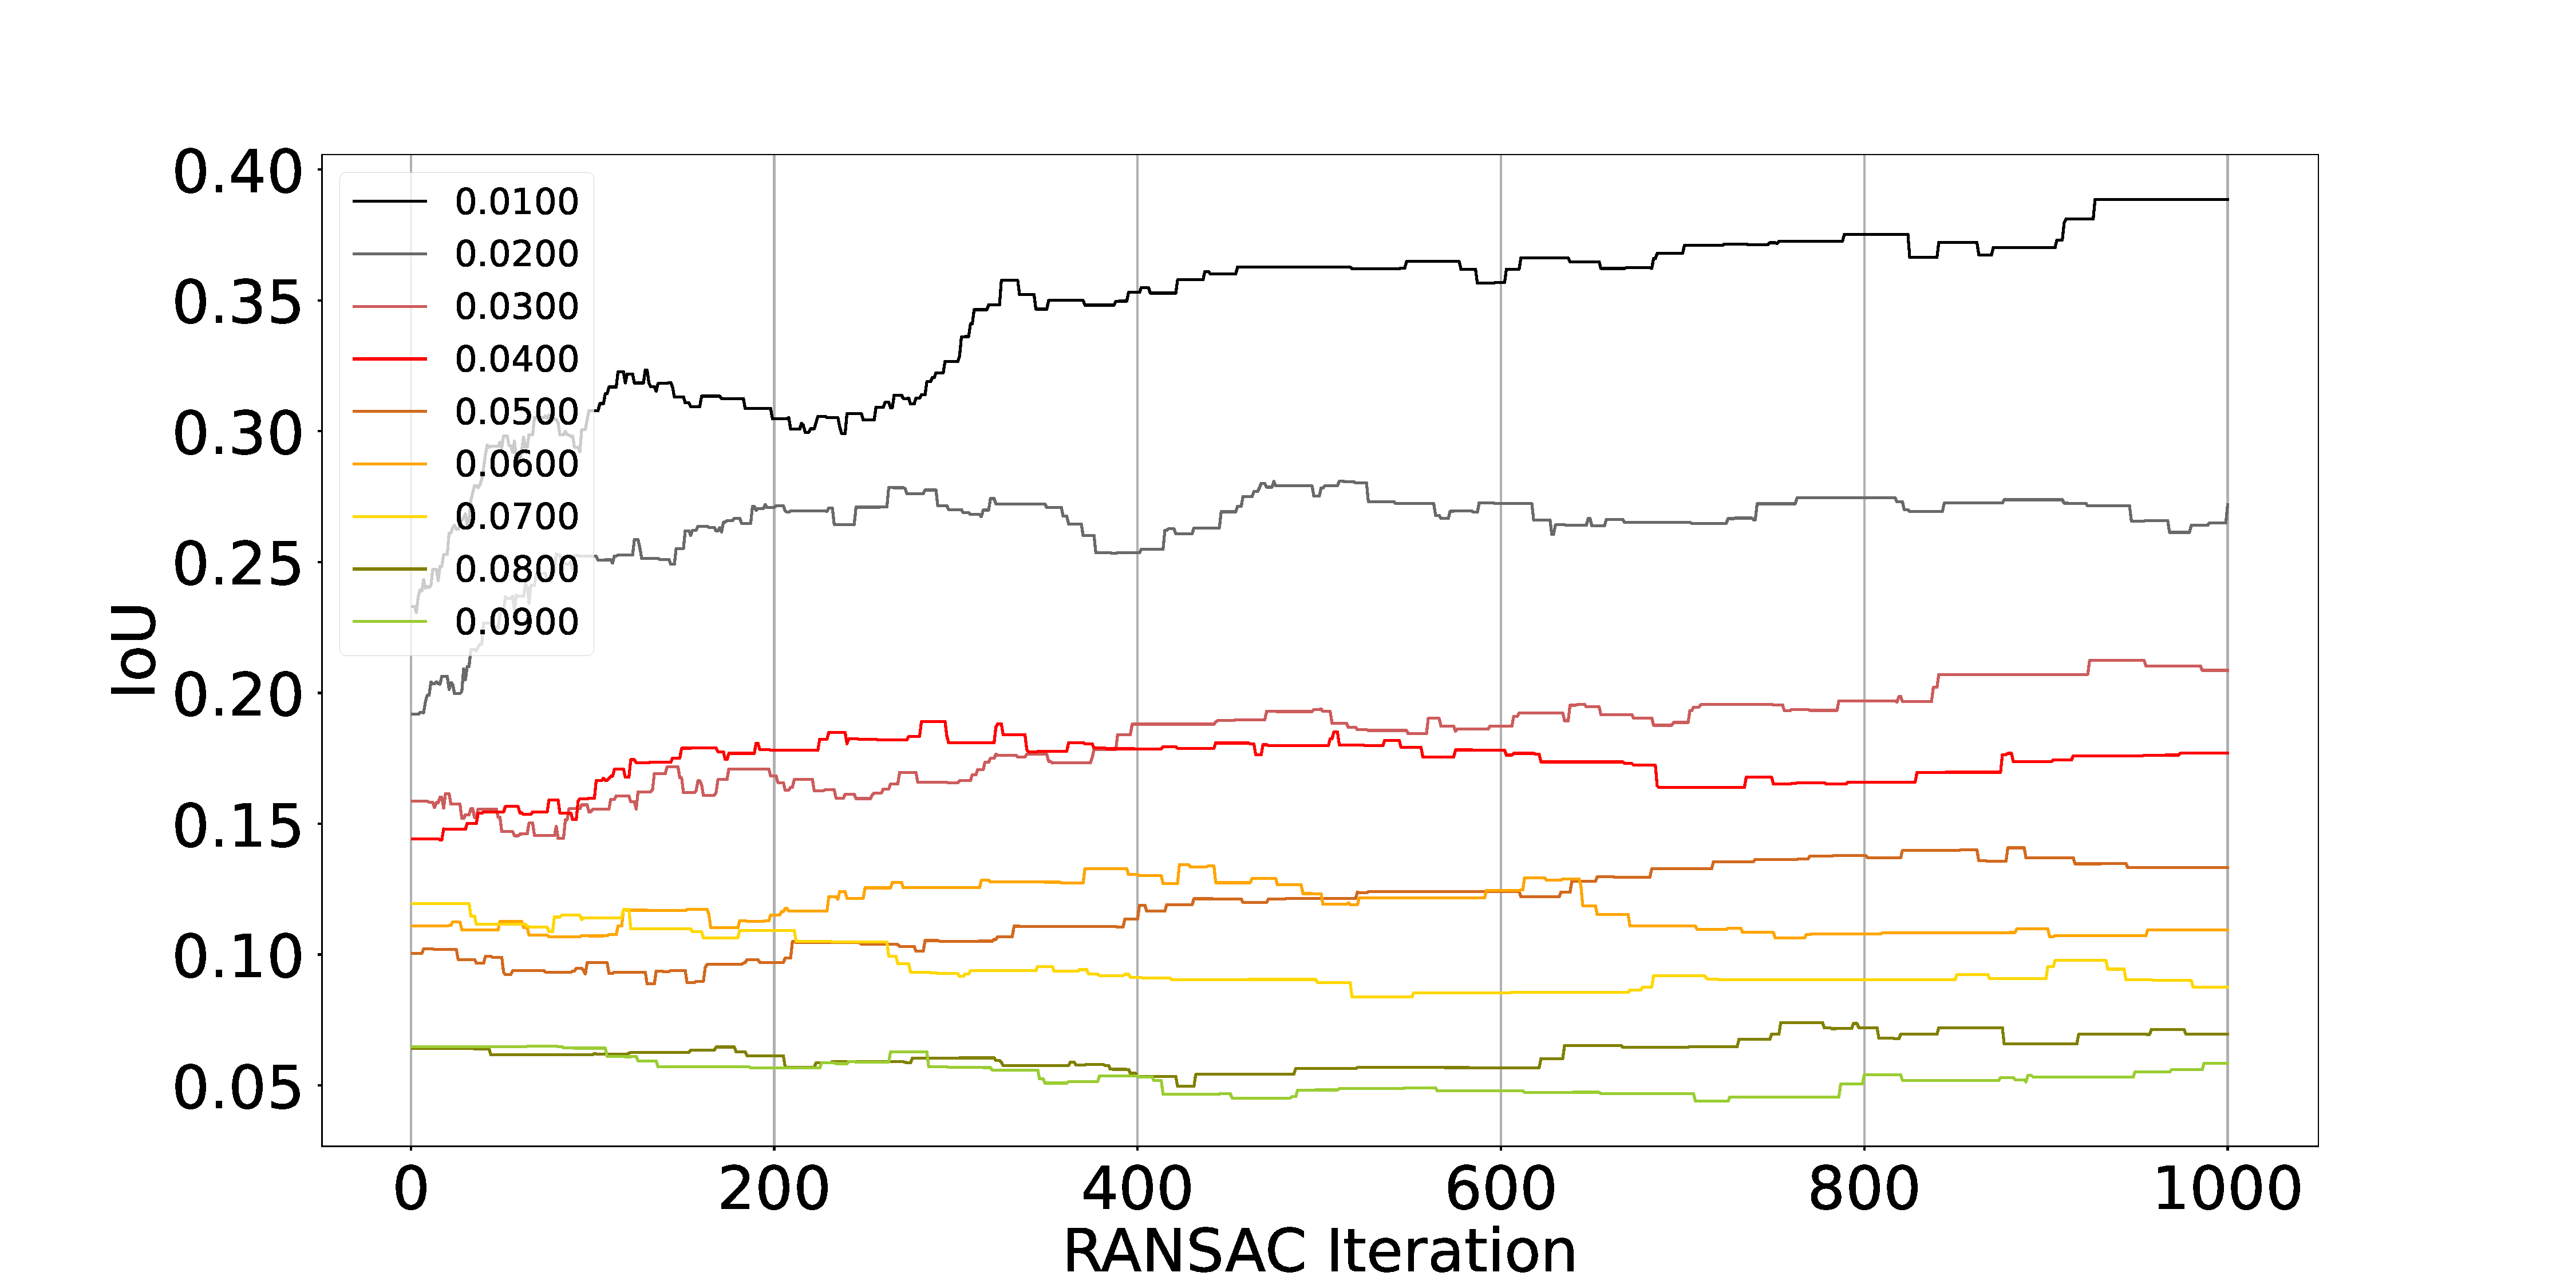
\includegraphics[width=0.48\textwidth]{images/segment_normal_noise_count_0.1_IoU_RANSAC_Iteration}
      \caption{Dependency of IoU of the best model from the number of iterations for synthetic segments for different levels of noise. It is worth noting that overall with the growth of the iteration number there is a slight, but noticeable improvement in IoU.}
      \label{fig:segment_normal_noise_count_0.1_IoU_RANSAC_Iteration}
  %\end{subfigure}
\end{figure}

\begin{figure}[!htb]
  \centering
  %\begin{subfigure}{0.48\textwidth}
  %    \centering
      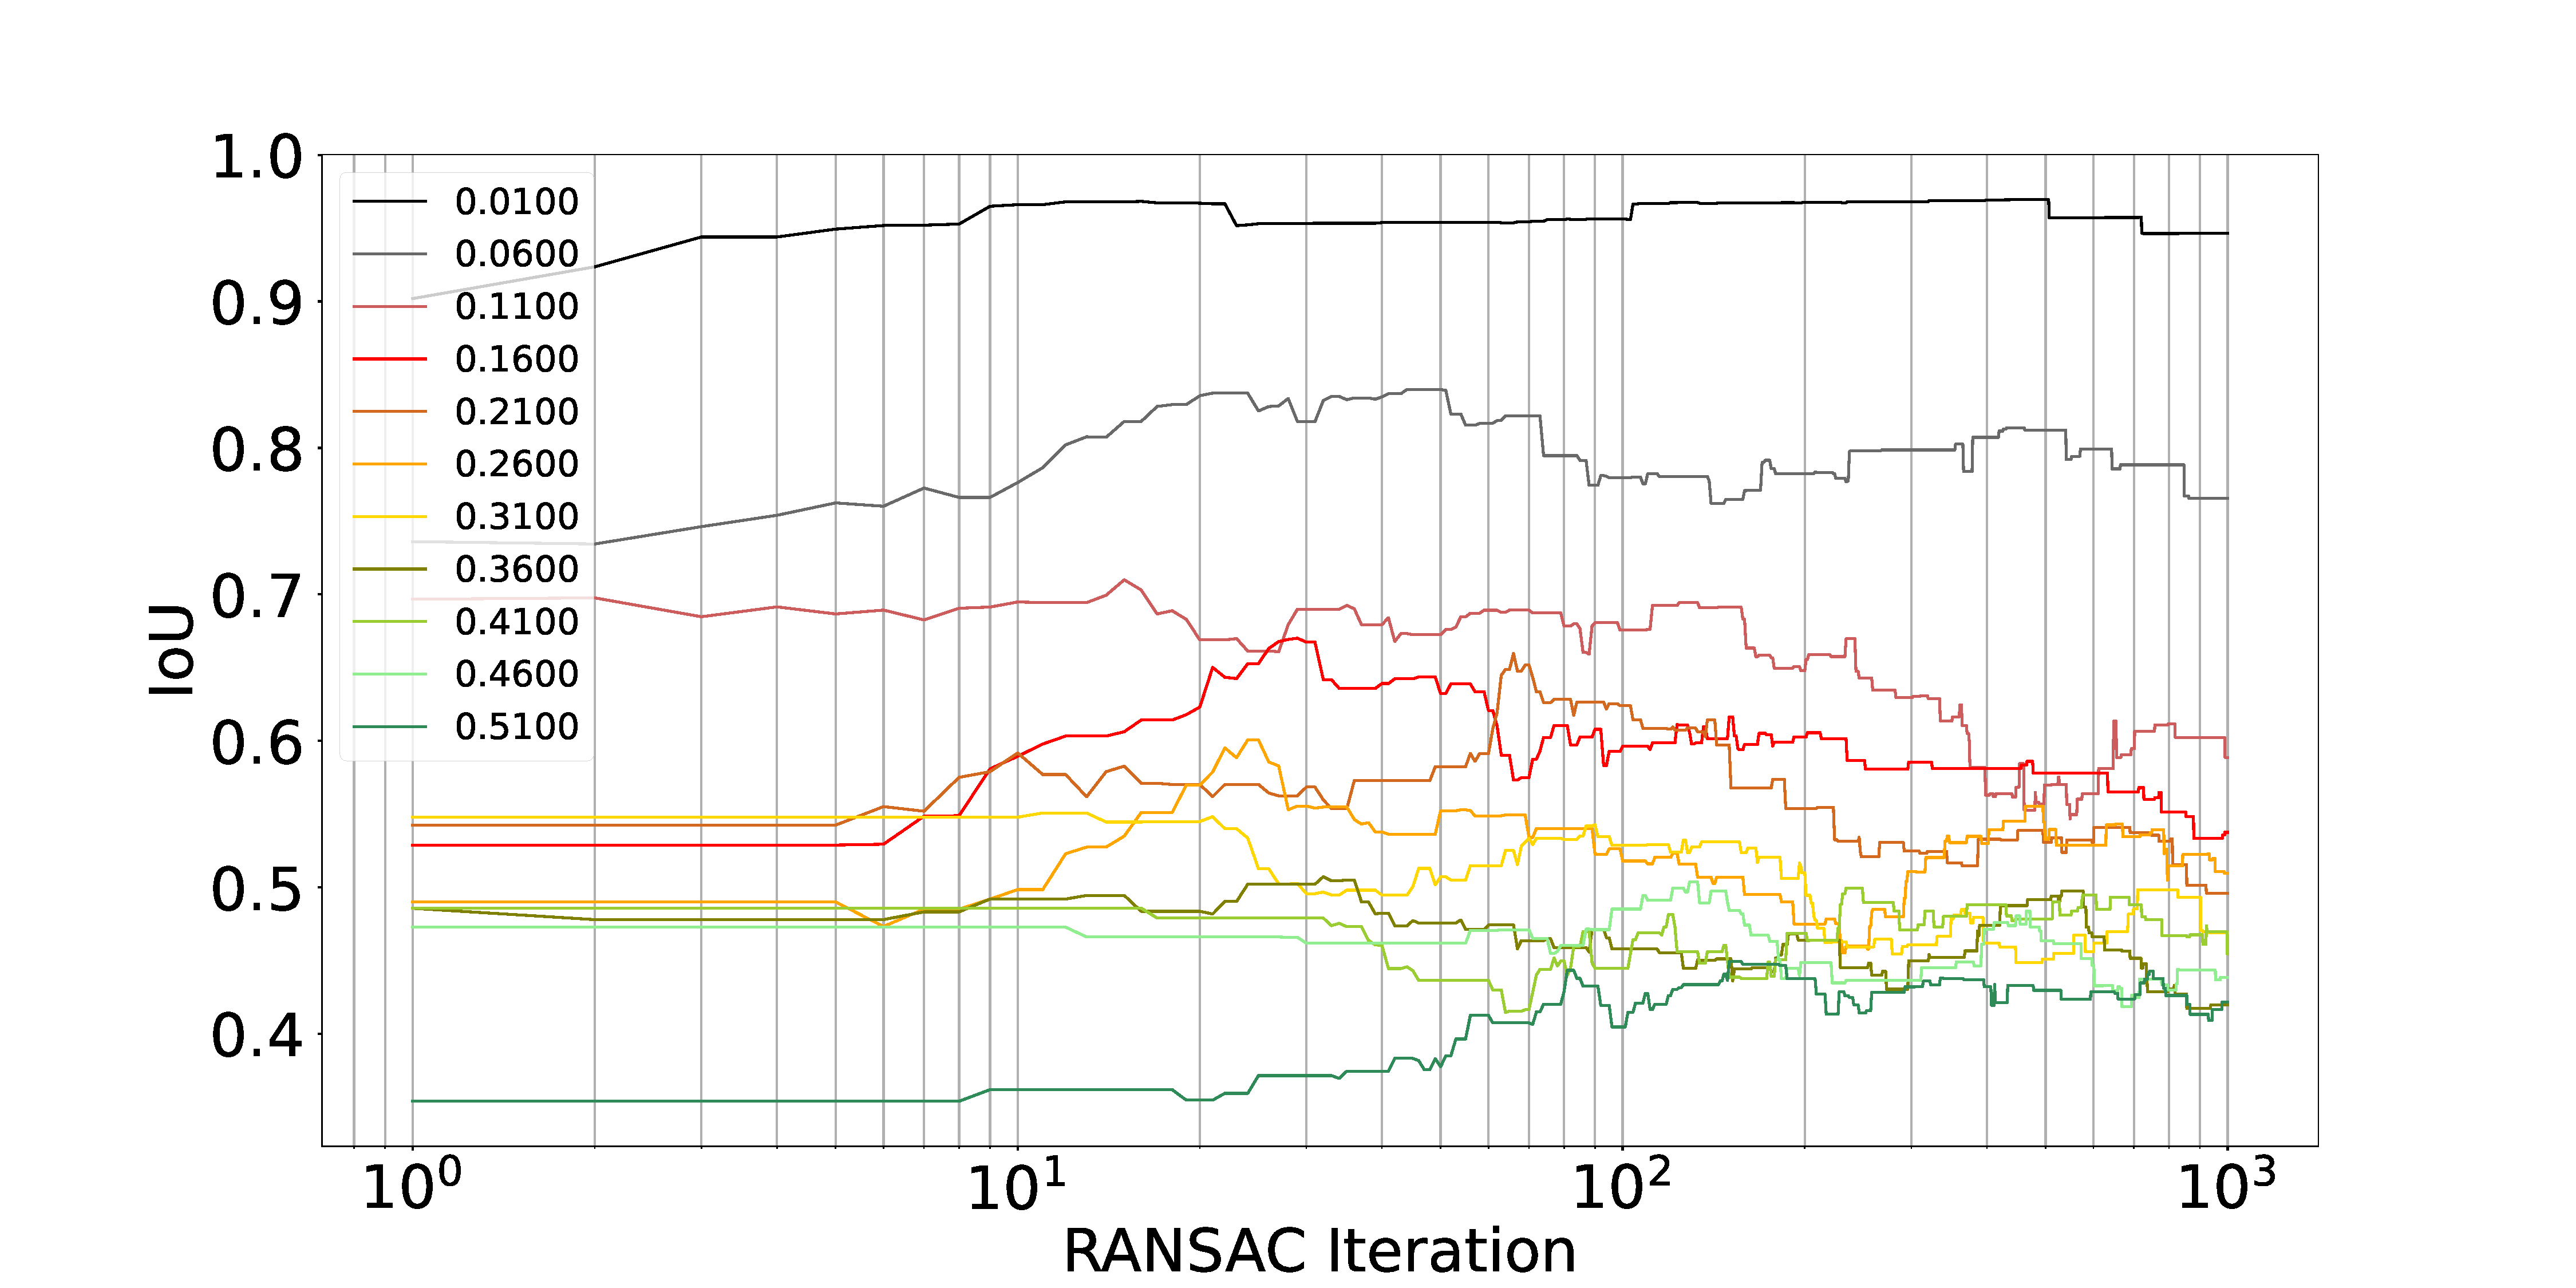
\includegraphics[width=0.48\textwidth]{images/normal_noise_count_0.1_IoU_RANSAC_Iteration}
      \caption{Dependency of IoU of the best model from the number of iterations for full synthetic ellipsoids for different levels of noise. x axis is logarithmic for better view. For light noise the IoU grows almost to 1.0 very rapidly (black line). For heavy noise the growth is much slower (green line).}
      \label{fig:normal_noise_count_0.1_IoU_RANSAC_Iteration}
  %\end{subfigure}
\end{figure}

% \begin{figure}[!htb]
%   \centering
%   %\begin{subfigure}{0.48\textwidth}
%   %    \centering
%       \includegraphics[width=0.48\textwidth]{gfx/graphs/synthetic_normal_noise_iou_iter_plot.pdf}
%       \caption{synthetic normal noise iou iter plot}
%       \label{fig_synthetic_normal_noise_iou_iter_plot}
%   %\end{subfigure}
% \end{figure}

% \begin{figure}[!htb]
%   \centering
%   %\begin{subfigure}{0.48\textwidth}
%   %    \centering
%       \includegraphics[width=0.48\textwidth]{gfx/graphs/synthetic_normal_noise_rel_vol_err_plot.pdf}
%       \caption{synthetic normal noise rel vol err plot}
%       \label{fig_synthetic_normal_noise_rel_vol_err_plot}
%   %\end{subfigure}
% \end{figure}

% \begin{figure}[!htb]
%   \centering
%   %\begin{subfigure}{0.48\textwidth}
%   %    \centering
%       \includegraphics[width=0.48\textwidth]{gfx/graphs/synthetic_segment_clean_models_iou_iter_plot.pdf}
%       \caption{synthetic segment clean models iou iter plot}
%       \label{fig_synthetic_segment_clean_models_iou_iter_plot}
%   %\end{subfigure}
% \end{figure}

% \begin{figure}[!htb]
%   \centering
%   %\begin{subfigure}{0.48\textwidth}
%   %    \centering
%       \includegraphics[width=0.48\textwidth]{gfx/graphs/synthetic_segment_clean_models_rel_vol_err_plot.pdf}
%       \caption{synthetic segment clean models rel vol err plot}
%       \label{fig_synthetic_segment_clean_models_rel_vol_err_plot}
%   %\end{subfigure}
% \end{figure}

% \begin{figure}[!htb]
%   \centering
%   %\begin{subfigure}{0.48\textwidth}
%   %    \centering
%       \includegraphics[width=0.48\textwidth]{gfx/graphs/synthetic_segment_normal_noise_iou_iter_plot.pdf}
%       \caption{synthetic segment normal noise iou iter plot}
%       \label{fig_synthetic_segment_normal_noise_iou_iter_plot}
%   %\end{subfigure}
% \end{figure}

\begin{figure}[!htb]
  \centering
  %\begin{subfigure}{0.48\textwidth}
  %    \centering
      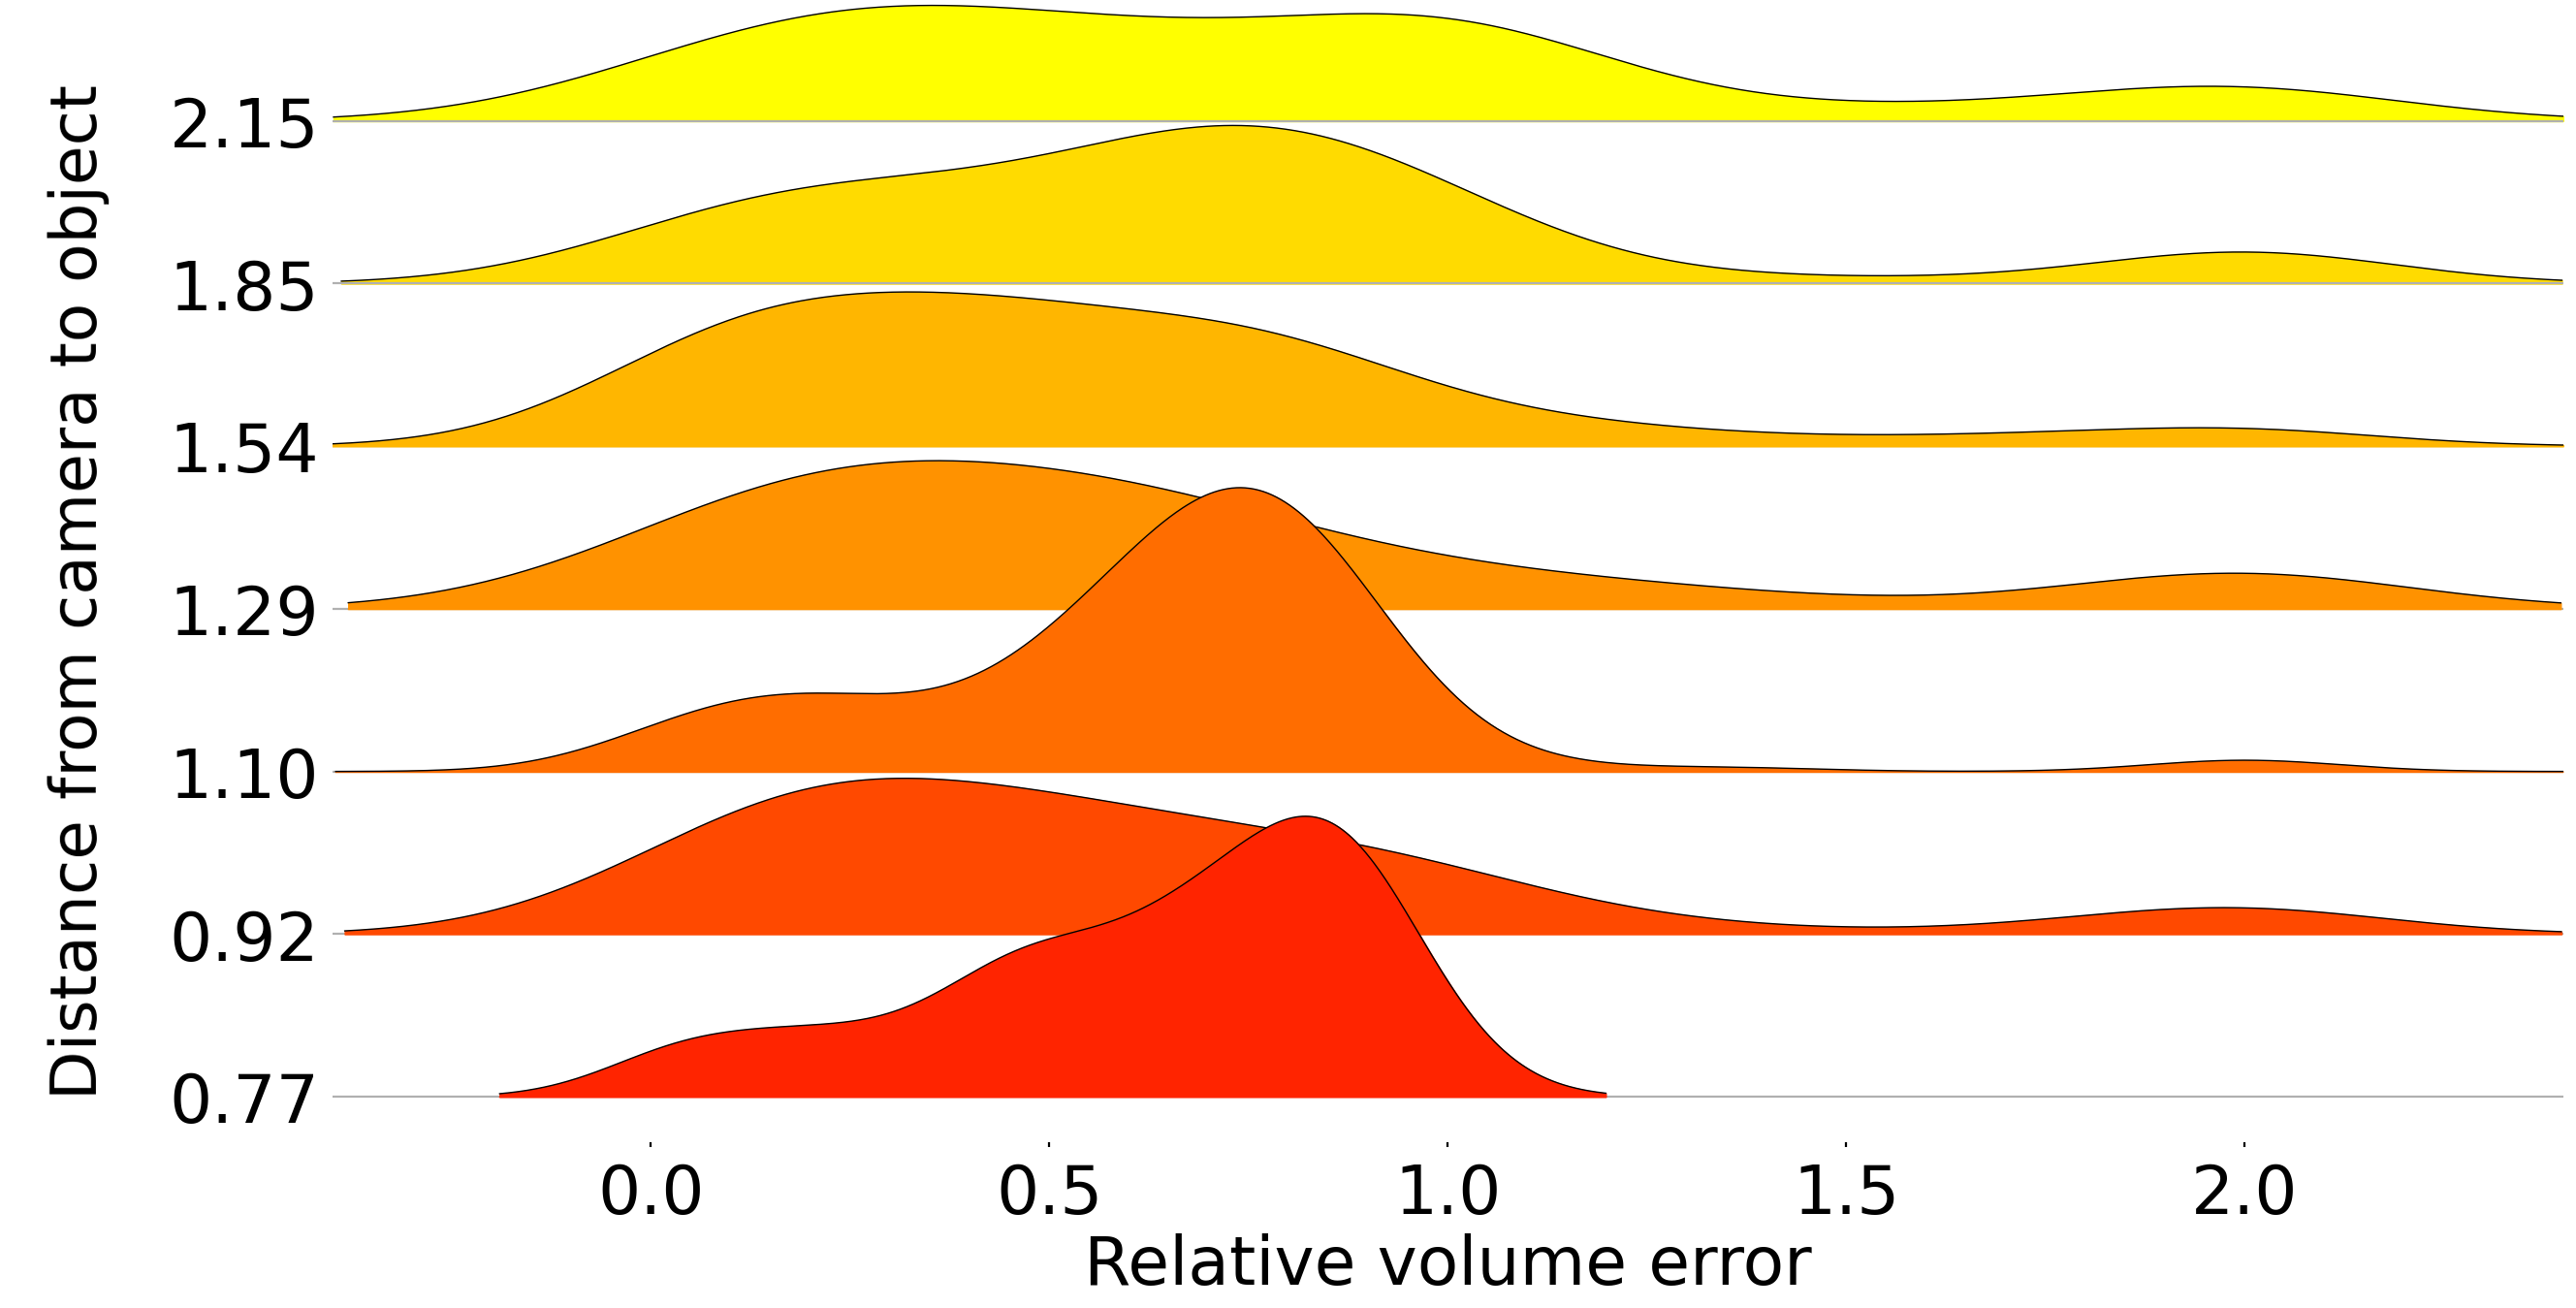
\includegraphics[width=0.48\textwidth]{images/res55.png}
      \caption{Distributions of Relative Volume Error for different distances from the camera for the point clouds filmed with 55 degrees between the camera direction and line of tomatoes}
      \label{fig:55res}
  %\end{subfigure}
\end{figure}

The best depth perception for Intel RealSense D435i is declared to belong to the range between 0.6 and 6 meters.
However, Figure \ref{fig:55res} as well as Figure \ref{fig:90res} suggest that the variance in the distribution in the relative volume error grows significantly beyond approximately 1.5 meters.
It can be explained by the decline in the infrared pattern density as the distance from the emitter increases.

%Tomatoes that are further than N meters were disregarded due to the poor data quality and the real greenhouse environment, where horizontal camera-to-tomato distance is limited by N meters.

%Tomatoes that are further than N meters were disregarded due to the poor data quality and the real greenhouse environment, where horizontal camera-to-tomato distance is limited by N meters.

The real applications are bounded by even more strict constraints in terms of the distance between the camera and the object.
Since the distance between the rows of the tomatoes is limited by approximately 2 \si{m}, and the vegetation should be taken into account, the distance between the camera and the plant in the real environment is supposed to be from 0.5 to 1.5 \si{m}.

\begin{figure}[!htb]
  \centering
  %\begin{subfigure}{0.48\textwidth}
  %    \centering
      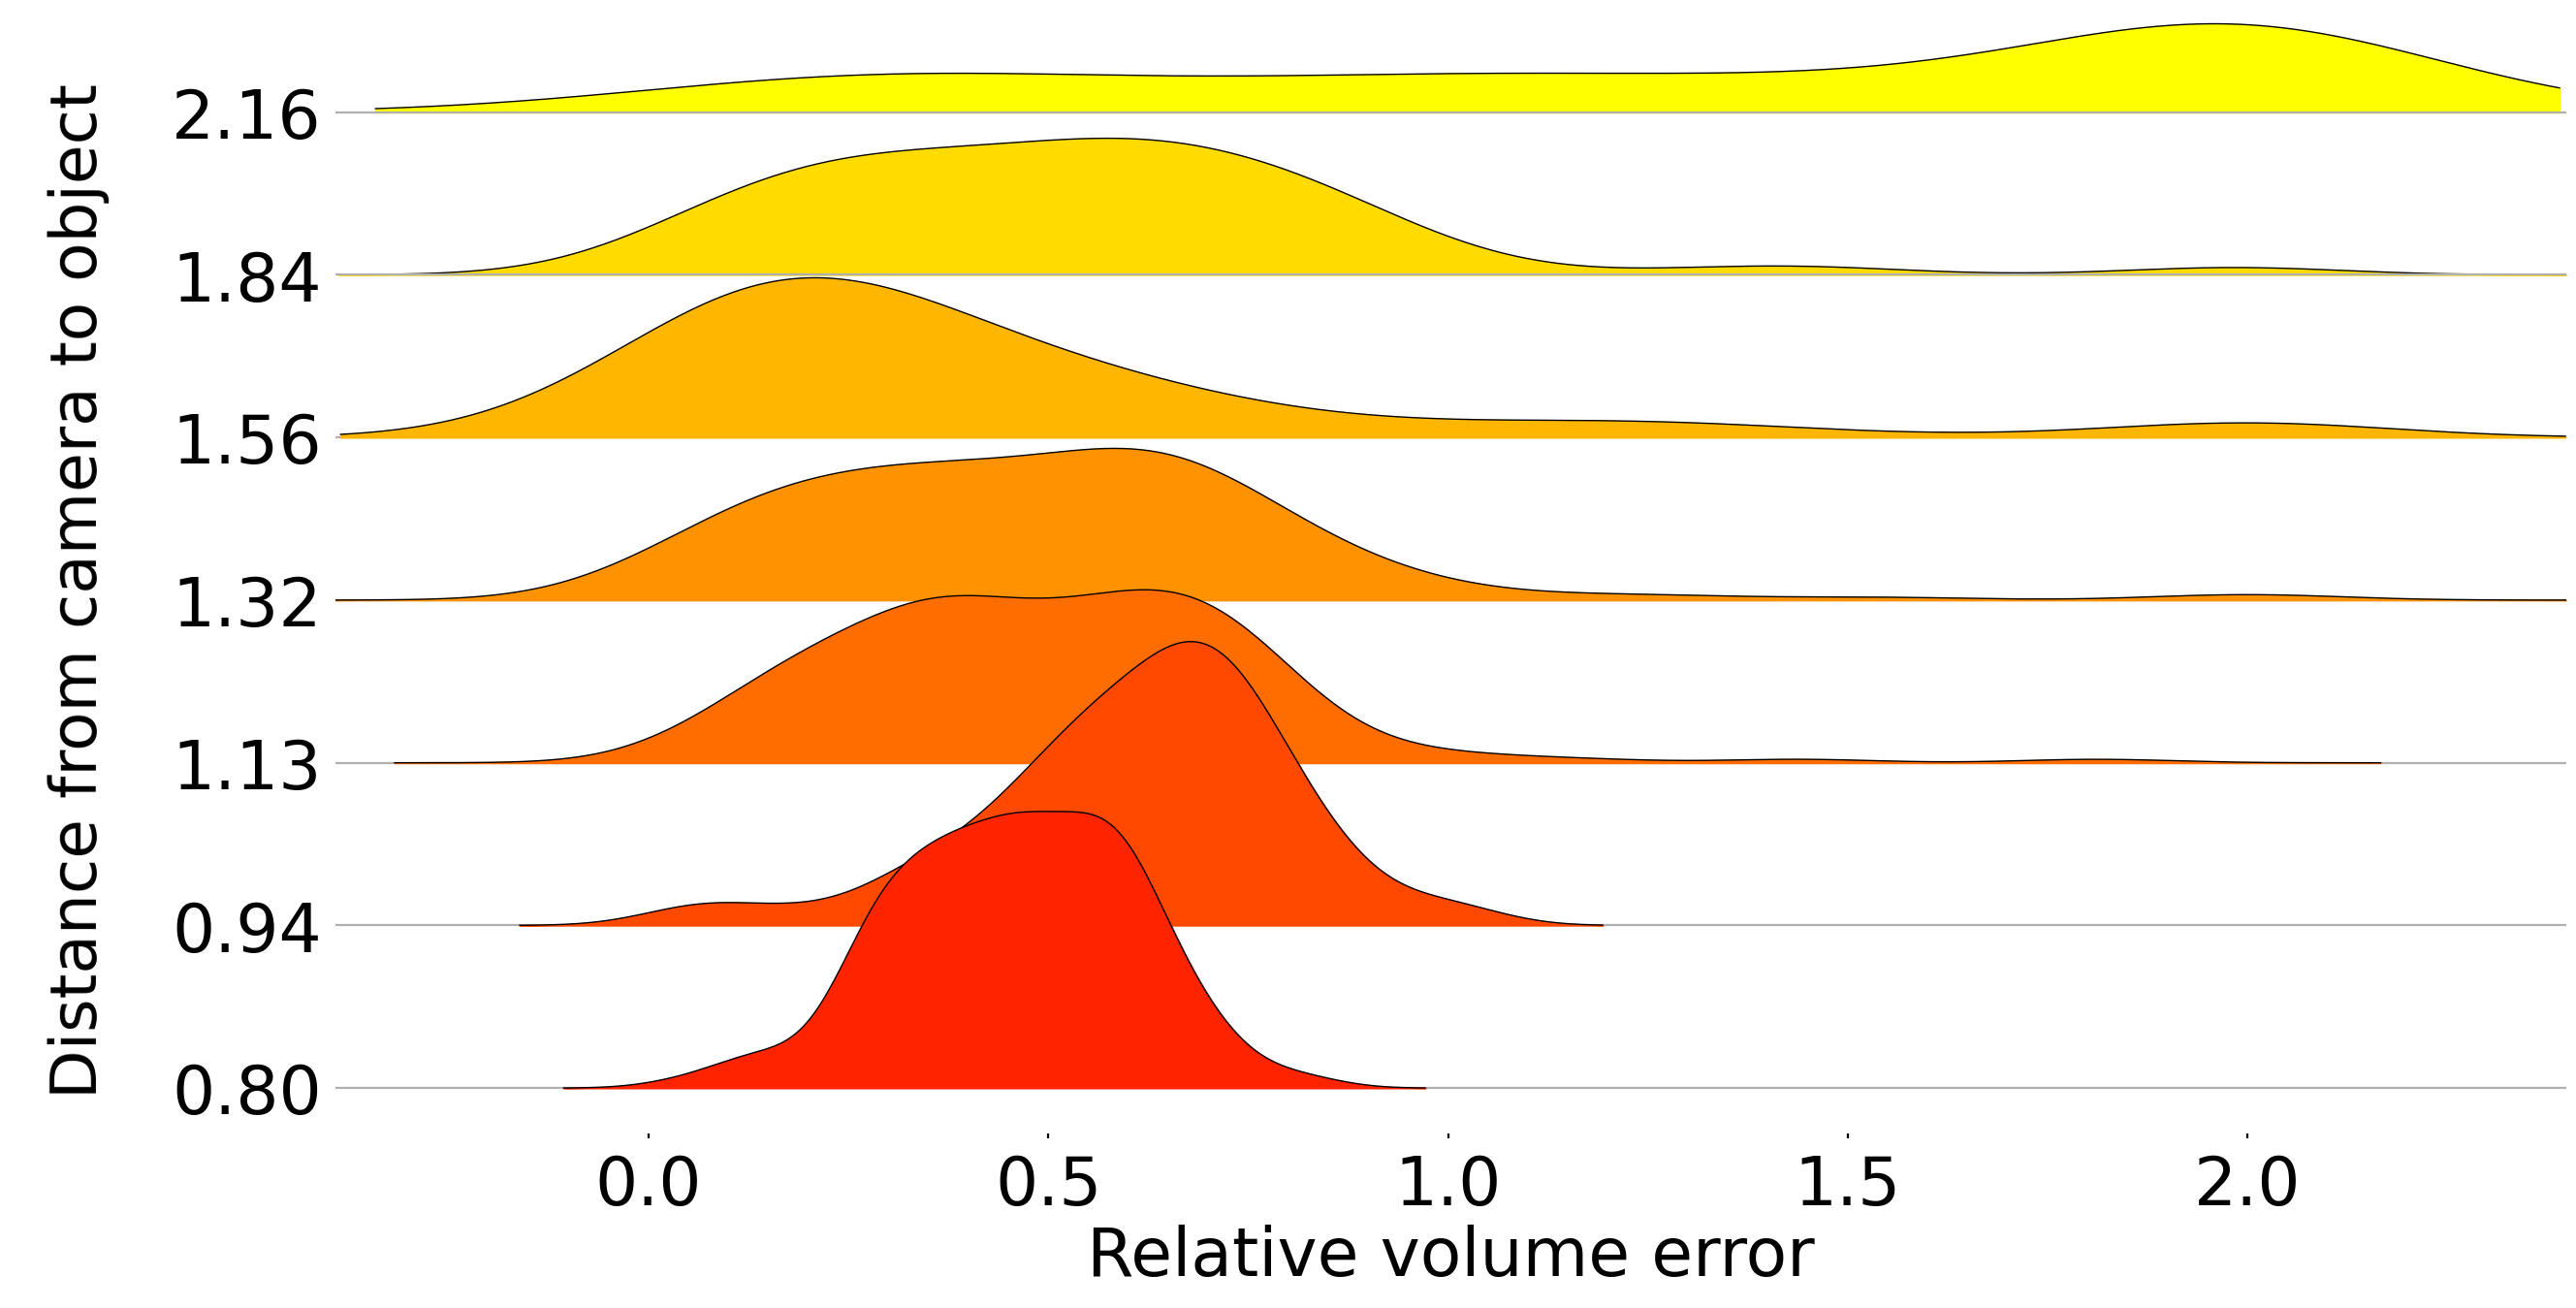
\includegraphics[width=0.48\textwidth]{images/res90.png}
      \caption{Distributions of Relative Volume Error for different distances from the camera for the point clouds filmed with 55 degrees between the camera direction and line of tomatoes}
      \label{fig:90res}
  %\end{subfigure}
\end{figure}

%\begin{figure}[!htb]
%  \centering
  %\begin{subfigure}{0.48\textwidth}
  %    \centering
%      \includegraphics[width=0.48\textwidth]{gfx/graphs/segment_normal_noise_total_rel_vol_iter_plot_log.pdf}
%      \caption{segment 90-120 noise 0.03 total vol but log }
%      \label{fig:segment_normal_noise_total_rel_vol_iter_plot_log}
  %\end{subfigure}
%\end{figure}

%\begin{figure}[!htb]
%  \centering
  %\begin{subfigure}{0.48\textwidth}
  %    \centering
%      \includegraphics[width=0.48\textwidth]{gfx/graphs/segment_normal_noise_total_rel_vol_iter_plot.pdf}
%      \caption{segment 90-120 noise 0.03 total vol}
%      \label{fig:segment_normal_noise_total_rel_vol_iter_plot}
  %\end{subfigure}
%\end{figure}

%\begin{figure}[!htb]
%  \centering
  %\begin{subfigure}{0.48\textwidth}
  %    \centering
 %     \includegraphics[width=0.48\textwidth]{gfx/graphs/normal_noise_total_rel_vol_iter_plot.pdf}
 %     \caption{normal noise 10 -30  total rel vol iter plot 0.4100 noise}
 %     \label{fig:normal_noise_total_rel_vol_iter_plot}
  %\end{subfigure}
%\end{figure}

\begin{figure}[!htb]
  \centering
  %\begin{subfigure}{0.48\textwidth}
  %    \centering
      \includegraphics[width=0.48\textwidth]{images/normal_noise_total_rel_vol_iter_plot_log.pdf}
      \caption{Dependency of the Total Relative Volume Error (sum over all the ellipsoids) on the number of iterations of RANSAC (logarithmic scale) for full noised synthetic ellipsoids. All the ellipsoids in the set have volume in the same order of magnitude. The noise level is 0.41.}
      \label{fig:normal_noise_total_rel_vol_iter_plot_log}
  %\end{subfigure}
\end{figure}

\begin{figure}[!htb]
  \centering
  %\begin{subfigure}{0.48\textwidth}
  %    \centering
      \includegraphics[width=0.48\textwidth]{images/errorbars.pdf}
      \caption{For each of the objects from the real dataset the volume was estimated for each of the point clouds.
      The average volumes with the error bars are listed along the axis represenating the distance from the camera to the object.
      The true volume for each of the tomatoes is marked with a thick black dot.}
      \label{fig:errorbars}
  %\end{subfigure}
\end{figure}

\begin{figure}[!htb]
  \centering
  %\begin{subfigure}{0.48\textwidth}
  %    \centering
      \includegraphics[width=0.48\textwidth]{images/rs-55_pcds_total_rel_vol_iter_plot.pdf}
      \caption{Dependency of the Total Relative Volume Error (sum over all the ellipsoids) on the number of iterations of RANSAC (logarithmic scale) for real data for different threshold values. The error clearly declines with the increase of the number of iterations.}
      \label{fig:wood_rs-55_pcds_total_rel_vol_iter_plot}
  %\end{subfigure}
\end{figure}

\begin{figure}[!htb]
  \centering
  %\begin{subfigure}{0.48\textwidth}
  %    \centering
      \includegraphics[width=0.48\textwidth]{images/wood_hist.pdf}
      \caption{The distribution of the relative volume error for all the tomatoes from the dataset. The mean value is 1.0020. No additional scaling was applied.}
      \label{fig:wood_hist}
  %\end{subfigure}
\end{figure}

It could be seen from the Figure \ref{fig:wood_hist} that despite high variance in the relative volume error the average measured volume matches the real one very precisely.
This result suggests that the method considered is applicable even under fairly noisy circumstances.

%\blue{
Figure \ref{fig:errorbars} presents the results of averaging the estimated volumes among all the point clouds for each tomato.
The real volume is marked with a black dot.
Despite high variance, the average volume is estimated with acceptable precision.
%}

%TODO: INSERT PLOT WITH IoU vs iter num for different noises

%TODO: INSERT IoU vs iter num for real tomatoes

%TODO: INSERT TABLE FROM THE END OF THE LAST PAGE OF THE PDF FROM THE DISCUSSION 31.10.2024

\section{Conclusion}
\label{sec_conclusion}

%\subsection{Conclusion}
%\label{sec_conclusion}

In this work an empirical study is carried out, aimed at examining the influence of noise on the performance of RANSAC method on quadric surfaces.
A method for synthetic data generation with ray tracing was developed.
The dependency of the error on the noise was examined on the synthetic point clouds.
Experiments on the real point clouds were carried out in the agricultural setting.
RANSAC for quadric surfaces was implemented in Python.

As one may expect, the results suggest that noisy data is more challenging for the algorithm.
The numerical evaluation of this phenomenon is given in the Results section \ref{sec_results}.
All in all, the qualitative findings are the following:
\begin{itemize}
  \item The number of inliers for the model is correlated with its quality in terms of the output metric. This correlation becomes less prominent with the growth of the noise.
  \item On the challenging data the number of iterations plays crucial role in the quality improvement, see Figure \ref{fig:normal_noise_total_rel_vol_iter_plot_log} and \ref{fig:segment_normal_noise_count_0.1_IoU_RANSAC_Iteration} for results on synthetic data.
  \item IoU cannot be used as a single criteria for quality assessment, see Figure \ref{fig:normal_noise_count_0.1_IoU_RANSAC_Iteration} and Figure \ref{fig:segment_normal_noise_count_0.1_IoU_RANSAC_Iteration} for a comparison of the plots for different noise levels.
  \item The quality of the output model declines with the growth of the distance from the sensor to the object. For the specific type of the camera that was used the cutoff distance that bounds the zone of reliable performance is nearly 1.5 meters.
  \item It was thus shown, that for the real data, which is the most challenging, RANSAC gives a high variance in the volume, but very small average error, which makes it applicable to the problem of yield estimation in the agricultural setting, see Figure \ref{fig:wood_rs-55_pcds_total_rel_vol_iter_plot}. The example of the algorithm's output is presented in the Figure \ref{fig:real_data_output}.
\end{itemize}

%All in all, a method was developed that gives precise estimate for the total volume of the group of tomatoes.

%%%%%%%%%%%%%%%%%%%%%%%%%%%%%%%%%%%%%%%%%%%%%%%%%%%%%%%%%%%%%%%%%%%%%%%%%%%%%%%%%%%%%%%%%%%%
%%%%%%%%%%%%%%%%%%%%%%%%%%%%%%%%%%%%%%%%%%%%%%%%%%%%%%% BIBLIOGRAPHY
\printbibliography

% =======================================================
%# Robot  #
% =======================================================
% \begin{figure}[!htb]
%     \centering
%     %\begin{subfigure}{0.48\textwidth}
%     %    \centering
%         \includegraphics[width=0.48\textwidth]{gfx/images/greenhouse/greenhouse_top_view_fixed-2.png}
%         \caption{Image taken in a greenhouse at the top of the plants.}
%         \label{fig_greenhouse_top_view}
%     %\end{subfigure}
% \end{figure}

%\printbibliography
    
%%%%%%%%%%%%%%%%%%%%%%%%%%%%%%%%%%%%%%%%%%%%%%%%%%%%%%%%%%%%%%%%%%%%%%%%%%%%%%%%%%%%%%%%%%%%%%%%%%%%%%%%%%%%%
%%%%%%%%%%%%%%%%%%%%%%%%%%%%%%%%%%%%%%%%%%%%%%%%%%%%%%%%%%%%%%%%%%%%%%%%%%%%%%%%%%%%%%%%%%%%%%%%%%%%%%%%%%%%%
%%%%%%%%%%%%%%%%%%%%%%%%%%%%%%%%%%%%%%%%%%%%%%%%%%%%%%%%%%%%%%%%%%%%%%%%%%%%%%%%%%%%%%%%%%%%%%%%%%%%%%%%%%%%%
%%%%%%%%%%%%%%%%%%%%%%%%%%%%%%%%%%%%%%%%%%%%%%%%%%%%%%%%%%%%%%%%%%%%%%%%%%%%%%%%%%%%%%%%%%%%%%%%%%%%%%%%%%%%%
%%%%%%%%%%%%%%%%%%%%%%%%%%%%%%%%%%%%%%%%%%%%%%%%%%%%%%%%%%%%%%%%%%%%%%%%%%%%%%%%%%%%%%%%%%%%%%%%%%%%%%%%%%%%%
%%%%%%%%%%%%%%%%%%%%%%%%%%%%%%%%%%%%%%%%%%%%%%%%%%%%%%%%%%%%%%%%%%%%%%%%%%%%%%%%%%%%%%%%%%%%%%%%%%%%%%%%%%%%%
%%%%%%%%%%%%%%%%%%%%%%%%%%%%%%%%%%%%%%%%%%%%%%%%%%%%%%%%%%%%%%%%%%%%%%%%%%%%%%%%%%%%%%%%%%%%%%%%%%%%%%%%%%%%%
%%%%%%%%%%%%%%%%%%%%%%%%%%%%%%%%%%%%%%%%%%%%%%%%%%%%%%%%%%%%%%%%%%%%%%%%%%%%%%%%%%%%%%%%%%%%%%%%%%%%%%%%%%%%%
%%%%%%%%%%%%%%%%%%%%%%%%%%%%%%%%%%%%%%%%%%%%%%%%%%%%%%%%%%%%%%%%%%%%%%%%%%%%%%%%%%%%%%%%%%%%%%%%%%%%%%%%%%%%%
%%%%%%%%%%%%%%%%%%%%%%%%%%%%%%%%%%%%%%%%%%%%%%%%%%%%%%%%%%%%%%%%%%%%%%%%%%%%%%%%%%%%%%%%%%%%%%%%%%%%%%%%%%%%%
%%%%%%%%%%%%%%%%%%%%%%%%%%%%%%%%%%%%%%%%%%%%%%%%%%%%%%%%%%%%%%%%%%%%%%%%%%%%%%%%%%%%%%%%%%%%%%%%%%%%%%%%%%%%%
%%%%%%%%%%%%%%%%%%%%%%%%%%%%%%%%%%%%%%%%%%%%%%%%%%%%%%%%%%%%%%%%%%%%%%%%%%%%%%%%%%%%%%%%%%%%%%%%%%%%%%%%%%%%%
%%%%%%%%%%%%%%%%%%%%%%%%%%%%%%%%%%%%%%%%%%%%%%%%%%%%%%%%%%%%%%%%%%%%%%%%%%%%%%%%%%%%%%%%%%%%%%%%%%%%%%%%%%%%%
%%%%%%%%%%%%%%%%%%%%%%%%%%%%%%%%%%%%%%%%%%%%%%%%%%%%%%%%%%%%%%%%%%%%%%%%%%%%%%%%%%%%%%%%%%%%%%%%%%%%%%%%%%%%%
%%%%%%%%%%%%%%%%%%%%%%%%%%%%%%%%%%%%%%%%%%%%%%%%%%%%%%%%%%%%%%%%%%%%%%%%%%%%%%%%%%%%%%%%%%%%%%%%%%%%%%%%%%%%%
%%%%%%%%%%%%%%%%%%%%%%%%%%%%%%%%%%%%%%%%%%%%%%%%%%%%%%%%%%%%%%%%%%%%%%%%%%%%%%%%%%%%%%%%%%%%%%%%%%%%%%%%%%%%%
%%%%%%%%%%%%%%%%%%%%%%%%%%%%%%%%%%%%%%%%%%%%%%%%%%%%%%%%%%%%%%%%%%%%%%%%%%%%%%%%%%%%%%%%%%%%%%%%%%%%%%%%%%%%%
%%%%%%%%%%%%%%%%%%%%%%%%%%%%%%%%%%%%%%%%%%%%%%%%%%%%%%%%%%%%%%%%%%%%%%%%%%%%%%%%%%%%%%%%%%%%%%%%%%%%%%%%%%%%%
%%%%%%%%%%%%%%%%%%%%%%%%%%%%%%%%%%%%%%%%%%%%%%%%%%%%%%%%%%%%%%%%%%%%%%%%%%%%%%%%%%%%%%%%%%%%%%%%%%%%%%%%%%%%%
%%%%%%%%%%%%%%%%%%%%%%%%%%%%%%%%%%%%%%%%%%%%%%%%%%%%%%%%%%%%%%%%%%%%%%%%%%%%%%%%%%%%%%%%%%%%%%%%%%%%%%%%%%%%%
%%%%%%%%%%%%%%%%%%%%%%%%%%%%%%%%%%%%%%%%%%%%%%%%%%%%%%%%%%%%%%%%%%%%%%%%%%%%%%%%%%%%%%%%%%%%%%%%%%%%%%%%%%%%%
%%%%%%%%%%%%%%%%%%%%%%%%%%%%%%%%%%%%%%%%%%%%%%%%%%%%%%%%%%%%%%%%%%%%%%%%%%%%%%%%%%%%%%%%%%%%%%%%%%%%%%%%%%%%%
%%%%%%%%%%%%%%%%%%%%%%%%%%%%%%%%%%%%%%%%%%%%%%%%%%%%%%%%%%%%%%%%%%%%%%%%%%%%%%%%%%%%%%%%%%%%%%%%%%%%%%%%%%%%%
%%%%%%%%%%%%%%%%%%%%%%%%%%%%%%%%%%%%%%%%%%%%%%%%%%%%%%%%%%%%%%%%%%%%%%%%%%%%%%%%%%%%%%%%%%%%%%%%%%%%%%%%%%%%%
%%%%%%%%%%%%%%%%%%%%%%%%%%%%%%%%%%%%%%%%%%%%%%%%%%%%%%%%%%%%%%%%%%%%%%%%%%%%%%%%%%%%%%%%%%%%%%%%%%%%%%%%%%%%%
%%%%%%%%%%%%%%%%%%%%%%%%%%%%%%%%%%%%%%%%%%%%%%%%%%%%%%%%%%%%%%%%%%%%%%%%%%%%%%%%%%%%%%%%%%%%%%%%%%%%%%%%%%%%%
%%%%%%%%%%%%%%%%%%%%%%%%%%%%%%%%%%%%%%%%%%%%%%%%%%%%%%%%%%%%%%%%%%%%%%%%%%%%%%%%%%%%%%%%%%%%%%%%%%%%%%%%%%%%%
%%%%%%%%%%%%%%%%%%%%%%%%%%%%%%%%%%%%%%%%%%%%%%%%%%%%%%%%%%%%%%%%%%%%%%%%%%%%%%%%%%%%%%%%%%%%%%%%%%%%%%%%%%%%%
%%%%%%%%%%%%%%%%%%%%%%%%%%%%%%%%%%%%%%%%%%%%%%%%%%%%%%%%%%%%%%%%%%%%%%%%%%%%%%%%%%%%%%%%%%%%%%%%%%%%%%%%%%%%%
%%%%%%%%%%%%%%%%%%%%%%%%%%%%%%%%%%%%%%%%%%%%%%%%%%%%%%%%%%%%%%%%%%%%%%%%%%%%%%%%%%%%%%%%%%%%%%%%%%%%%%%%%%%%%
%%%%%%%%%%%%%%%%%%%%%%%%%%%%%%%%%%%%%%%%%%%%%%%%%%%%%%%%%%%%%%%%%%%%%%%%%%%%%%%%%%%%%%%%%%%%%%%%%%%%%%%%%%%%%
%%%%%%%%%%%%%%%%%%%%%%%%%%%%%%%%%%%%%%%%%%%%%%%%%%%%%%%%%%%%%%%%%%%%%%%%%%%%%%%%%%%%%%%%%%%%%%%%%%%%%%%%%%%%%

Ellipsoidal objects volume estimation by combining detection with RANSAC

I. S. Ryakin1,2, I. V. Osokin2, P. V. Osinenko2
1Moscow Institute of Physics and Technology
2Skolkovo Institute of Science and Technology

A method of ellipsoid volume estimation by noisy point cloud data is proposed. It relies on the combination of RGB and depth data. Specifically, it consists of two parts: detecting the objects in the RGB image, that is registered to the point cloud from a depth camera, and fitting ellipsoids to the corresponding subsets of that point cloud. The proposed method was tested on synthetic data and real data in agricultural context. Its main feature is that it is suitable for the real-world environments. For industrial applications, such as modern tomato greenhouses, it means that the tomatoes are not supposed to be manually picked.
	Volume estimation is a fundamental problem that has to be solved in a variety of real-world scenarios, ranging from agriculture[1,2] to medicine [3]. In contrast to many modern approaches, the proposed one does not rely on the contrastive background or an expensive setup with multispectral cameras. For the real experiments Intel RealSense D435i camera was used. The method's performance was evaluated on both synthetic and real data in terms of the Intersection over Union (IoU) between the predicted ellipsoid and the real one, volume error and processing time. The dependence of the output quality on the parameters, such as number of RANSAC iterations and inlier threshold, is presented. The method is compared with three other modern algorithms, showing superior performance on the complex real-world data. It is lightweight enough to be used on an autonomous agricultural robot with a user-grade laptop on board. To our knowledge there are no works that combine NN-based detection with robust volume estimation.


Figure 1. Proposed algorithm. First, RGB and point cloud data are obtained with distinct, but registered sensors. Second, NN-based detection is performed and point clouds corresponding to individual objects are extracted. Finally, RANSAC algorithm is used to fir the proper ellipsoid models to them, consisting of repetitive subsampling and model evaluation.

The contributions of this paper are as follows. A dataset of point clouds with tomatoes was collected in the environment closely mimicking the real greenhouse. The dataset was marked, meaning that the tomato models were hand-fitted to the point clouds. Synthetic data was generated. RANSAC for quadric surfaces was implemented in Python. A pipeline consisting of YOLO [4] detection with subsequent point cloud cropping and RANSAC inference was realized. Numerical experiments were conducted. A comparison with modern approaches to ellipsoid estimation was made. It was thus shown that good enough performance could be achieved with the means of an autonomous robot and relatively cheap camera setup. 
The data was recorded data using both RGB and Depth channels, synchronized via standard RealSense SDK methods. Each tomato was physically marked for identification during post-processing.
The lighting conditions were consistent, as the room was equipped with a window that blocks infrared light, and the overcast weather prevented direct sunlight.
	The proposed method was compared with three modern approaches on both synthetic and real data from the agricultural context. The first one is [5]. In this work a Bayesian approach to ellipsoid fitting was taken, that generalizes well even to higher dimensions. This algorithm maximizes the probability of the output model given the data, thus being robust to noise and out-of-distribution points. The second one is the implementation of Matlab Ellipsoid Fit [6]. In this work the problem of ellipsoid obtainment is approached with Linear Least Squares (LLSQ), followed by bringing the ellipsoid to the form of a quadric surface. Finally, the proposed approach was compared with [7]. The authors noted that in a lot of RANSAC implementations either the geometrical or algebraic distance was used in order to evaluate the quality of the model. An alternative approach was proposed, relying on the combination of the axial and Sampson distance, which gave high robustness against outliers and competitive processing time.
The results are presented in the Tables 2, 3, 4 and 5. First, let us observe the metrics for different number of iterations for the best threshold are presented in the Table 1.


Iterations	IoU	Volume Error
10	0.2125	0.5084
100	0.2145	0.3587
1000	0.2164	0.2459

Table 1. IoU and Volume Error for different number of RANSAC iterations on real data

Let us compare the performance of the proposed method with the other algorithms, see Tables 2, 3, 4 and 5.

	Clean Models	Normal Noise
	IoU	Volume Error	Time	IoU	Volume Error	Time
Bayfit	0.0078	0.1164	1.5849	0.0104	2.88e+25	0.3709
CAS	1.0	0.0	0.0037	0.7202	0.164	0.0174
Matlab Ellipsoid Fit	1.0	0.0	0.0003	0.8024	0.0925	0.0003
RANSAC (ours)	1.0	0.0	0.0297	0.5101	1.17	0.0297
Table 2. The comparison of the algorithms on clean and noisy full ellipsoids

	Segment Clean Models	Segment Normal Noise
	IoU	Volume Error	Time	IoU	Volume Error	Time
Bayfit	0.0005	0.3985	1.1149	N/A	N/A	N/A
CAS	0.9899	0.01	0.0027	0.2054	4.0796	0.0029
Matlab Ellipsoid Fit	0.8447	20.8465	0.0006	0.1387	0.426	0.0005
RANSAC (ours)	0.9697	0.0192	0.0287	0.1985	2.1242	0.0298
Table 3. The comparison of the algorithms on Segment Clean data and Segment Normal Noise. N/A means that the algorithm did not provide a result

	Real Data
	IoU	Volume Error	Time
Bayfit	0.0185	0.9629	0.0657
CAS	0.1501	18.3553	0.0037
Matlab Ellipsoid Fit	0.0003	7.1066	0.0010
RANSAC (ours)	0.2237	0.7617	0.0254

Table 4. Real Data Results and Iterations


	Year	Lang	Clean	Noisy	Clean Segm	Noisy Segm	Real Data
Bayfit	2024	Matlab	Yes	Yes	Yes	No	Yes
CAS	2022	Matlab	Yes	Yes	Yes	Yes	Yes
Matlab Ellipsoid Fit	2018	Matlab/Python	Yes	Yes	Yes	Yes	Yes
RANSAC (ours)	2024	Python	Yes	Yes	Yes	Yes	Yes
Table 5. Summary of the methods. Yes and No for different data types denote if the method is working with them or not

On some of the synthetic data the proposed method performs worse than the other methods, see Normal Noise IoU, where Matlab Ellipsoid Fit gives higher IoU. However, on the most challenging sort of data, which is the real ellipsoids, the proposed method shows superior performance in terms of both IoU and volume error. Moreover, it could be noted that the average volume for a group of tomatoes closely matches real values, despite high variance in individual outputs, see Figure 2.

Figure 2.  Distribution of the predicted volume divided by the real
volume for all the tomatoes in the real data. Despite the variance
being considerable, the mean value is nearly 1.05, which means
that the main metric that the potential user will be interested in,
which is the volume estimation precision, is high.

Overall, a method of ellipsoid volume estimation was developed and tested in the real environment. Synthetic data was generated with gradual increase in complexity. A real dataset of point clouds and corresponding RGB images was gathered and marked. The dependence of the quality of the method's output on the iterations number was evaluated in numerical experiments, showing minimal average relative volume estimation error of 0.25. The comparison of the method with three alternative approaches was made, showing superior performance on the real data both in terms of IoU and volume error. It was thus shown that the proposed method can be applied to the real-world ellipsoid volume estimation.
References
    1. Nakaguro Y. et al. Volumetric 3D Reconstruction and Parametric Shape Modeling from RGB-D Sequences //Image Analysis and Processing—ICIAP 2015: 18th International Conference, Genoa, Italy, September 7-11, 2015, Proceedings, Part I 18. – Springer International Publishing, 2015. – P. 500-516. 
    2. Chaivivatrakul S. et al.TOWARDS AUTOMATED CROP YIELD ESTIMATION.
    3. Rodriguez E. et al. Prostate volume estimation using the ellipsoid formula consistently underestimates actual gland size //The Journal of urology. – 2008. – V. 179. – №. 2. – P. 501-503.
    4. Redmon J. et al. You only look once: Unified, real-time object detection //Proceedings of the IEEE conference on computer vision and pattern recognition. – 2016. – P. 779-788.
    5. Zhao M. et al. A Bayesian Approach Toward Robust Multidimensional Ellipsoid-Specific Fitting //IEEE Transactions on Pattern Analysis and Machine Intelligence. – 2024.
    6. Yury. Ellipsoid fit // MATLAB Central File Exchange : [Electronic resource]. URL: https://www.mathworks.com/matlabcentral/fileexchange/24693-ellipsoid-fit (accessed: 02.03.2025).
    7. Han M. et al. Robust ellipsoid fitting using combination of axial and Sampson distances //IEEE Transactions on Instrumentation and Measurement. – 2023. – V. 72. – P. 1-14.





%%%%%%%%%%%%%%%%%%%%%%%%%%%%%%%%%%%%%%%%%%%%%%%%%%%%%%%%%%%%%%%%%%%%%%%%%%%%%%%%%%%%%%%%%%%%%%%%%%%%%%%%%%%%%
%%%%%%%%%%%%%%%%%%%%%%%%%%%%%%%%%%%%%%%%%%%%%%%%%%%%%%%%%%%%%%%%%%%%%%%%%%%%%%%%%%%%%%%%%%%%%%%%%%%%%%%%%%%%%
%%%%%%%%%%%%%%%%%%%%%%%%%%%%%%%%%%%%%%%%%%%%%%%%%%%%%%%%%%%%%%%%%%%%%%%%%%%%%%%%%%%%%%%%%%%%%%%%%%%%%%%%%%%%%
%%%%%%%%%%%%%%%%%%%%%%%%%%%%%%%%%%%%%%%%%%%%%%%%%%%%%%%%%%%%%%%%%%%%%%%%%%%%%%%%%%%%%%%%%%%%%%%%%%%%%%%%%%%%%
%%%%%%%%%%%%%%%%%%%%%%%%%%%%%%%%%%%%%%%%%%%%%%%%%%%%%%%%%%%%%%%%%%%%%%%%%%%%%%%%%%%%%%%%%%%%%%%%%%%%%%%%%%%%%
%%%%%%%%%%%%%%%%%%%%%%%%%%%%%%%%%%%%%%%%%%%%%%%%%%%%%%%%%%%%%%%%%%%%%%%%%%%%%%%%%%%%%%%%%%%%%%%%%%%%%%%%%%%%%
%%%%%%%%%%%%%%%%%%%%%%%%%%%%%%%%%%%%%%%%%%%%%%%%%%%%%%%%%%%%%%%%%%%%%%%%%%%%%%%%%%%%%%%%%%%%%%%%%%%%%%%%%%%%%
%%%%%%%%%%%%%%%%%%%%%%%%%%%%%%%%%%%%%%%%%%%%%%%%%%%%%%%%%%%%%%%%%%%%%%%%%%%%%%%%%%%%%%%%%%%%%%%%%%%%%%%%%%%%%
%%%%%%%%%%%%%%%%%%%%%%%%%%%%%%%%%%%%%%%%%%%%%%%%%%%%%%%%%%%%%%%%%%%%%%%%%%%%%%%%%%%%%%%%%%%%%%%%%%%%%%%%%%%%%
%%%%%%%%%%%%%%%%%%%%%%%%%%%%%%%%%%%%%%%%%%%%%%%%%%%%%%%%%%%%%%%%%%%%%%%%%%%%%%%%%%%%%%%%%%%%%%%%%%%%%%%%%%%%%
%%%%%%%%%%%%%%%%%%%%%%%%%%%%%%%%%%%%%%%%%%%%%%%%%%%%%%%%%%%%%%%%%%%%%%%%%%%%%%%%%%%%%%%%%%%%%%%%%%%%%%%%%%%%%
%%%%%%%%%%%%%%%%%%%%%%%%%%%%%%%%%%%%%%%%%%%%%%%%%%%%%%%%%%%%%%%%%%%%%%%%%%%%%%%%%%%%%%%%%%%%%%%%%%%%%%%%%%%%%
%%%%%%%%%%%%%%%%%%%%%%%%%%%%%%%%%%%%%%%%%%%%%%%%%%%%%%%%%%%%%%%%%%%%%%%%%%%%%%%%%%%%%%%%%%%%%%%%%%%%%%%%%%%%%
%%%%%%%%%%%%%%%%%%%%%%%%%%%%%%%%%%%%%%%%%%%%%%%%%%%%%%%%%%%%%%%%%%%%%%%%%%%%%%%%%%%%%%%%%%%%%%%%%%%%%%%%%%%%%
%%%%%%%%%%%%%%%%%%%%%%%%%%%%%%%%%%%%%%%%%%%%%%%%%%%%%%%%%%%%%%%%%%%%%%%%%%%%%%%%%%%%%%%%%%%%%%%%%%%%%%%%%%%%%
%%%%%%%%%%%%%%%%%%%%%%%%%%%%%%%%%%%%%%%%%%%%%%%%%%%%%%%%%%%%%%%%%%%%%%%%%%%%%%%%%%%%%%%%%%%%%%%%%%%%%%%%%%%%%
%%%%%%%%%%%%%%%%%%%%%%%%%%%%%%%%%%%%%%%%%%%%%%%%%%%%%%%%%%%%%%%%%%%%%%%%%%%%%%%%%%%%%%%%%%%%%%%%%%%%%%%%%%%%%
%%%%%%%%%%%%%%%%%%%%%%%%%%%%%%%%%%%%%%%%%%%%%%%%%%%%%%%%%%%%%%%%%%%%%%%%%%%%%%%%%%%%%%%%%%%%%%%%%%%%%%%%%%%%%
%%%%%%%%%%%%%%%%%%%%%%%%%%%%%%%%%%%%%%%%%%%%%%%%%%%%%%%%%%%%%%%%%%%%%%%%%%%%%%%%%%%%%%%%%%%%%%%%%%%%%%%%%%%%%
%%%%%%%%%%%%%%%%%%%%%%%%%%%%%%%%%%%%%%%%%%%%%%%%%%%%%%%%%%%%%%%%%%%%%%%%%%%%%%%%%%%%%%%%%%%%%%%%%%%%%%%%%%%%%
%%%%%%%%%%%%%%%%%%%%%%%%%%%%%%%%%%%%%%%%%%%%%%%%%%%%%%%%%%%%%%%%%%%%%%%%%%%%%%%%%%%%%%%%%%%%%%%%%%%%%%%%%%%%%
%%%%%%%%%%%%%%%%%%%%%%%%%%%%%%%%%%%%%%%%%%%%%%%%%%%%%%%%%%%%%%%%%%%%%%%%%%%%%%%%%%%%%%%%%%%%%%%%%%%%%%%%%%%%%
%%%%%%%%%%%%%%%%%%%%%%%%%%%%%%%%%%%%%%%%%%%%%%%%%%%%%%%%%%%%%%%%%%%%%%%%%%%%%%%%%%%%%%%%%%%%%%%%%%%%%%%%%%%%%
%%%%%%%%%%%%%%%%%%%%%%%%%%%%%%%%%%%%%%%%%%%%%%%%%%%%%%%%%%%%%%%%%%%%%%%%%%%%%%%%%%%%%%%%%%%%%%%%%%%%%%%%%%%%%
%%%%%%%%%%%%%%%%%%%%%%%%%%%%%%%%%%%%%%%%%%%%%%%%%%%%%%%%%%%%%%%%%%%%%%%%%%%%%%%%%%%%%%%%%%%%%%%%%%%%%%%%%%%%%
%%%%%%%%%%%%%%%%%%%%%%%%%%%%%%%%%%%%%%%%%%%%%%%%%%%%%%%%%%%%%%%%%%%%%%%%%%%%%%%%%%%%%%%%%%%%%%%%%%%%%%%%%%%%%
%%%%%%%%%%%%%%%%%%%%%%%%%%%%%%%%%%%%%%%%%%%%%%%%%%%%%%%%%%%%%%%%%%%%%%%%%%%%%%%%%%%%%%%%%%%%%%%%%%%%%%%%%%%%%
%%%%%%%%%%%%%%%%%%%%%%%%%%%%%%%%%%%%%%%%%%%%%%%%%%%%%%%%%%%%%%%%%%%%%%%%%%%%%%%%%%%%%%%%%%%%%%%%%%%%%%%%%%%%%
%%%%%%%%%%%%%%%%%%%%%%%%%%%%%%%%%%%%%%%%%%%%%%%%%%%%%%%%%%%%%%%%%%%%%%%%%%%%%%%%%%%%%%%%%%%%%%%%%%%%%%%%%%%%%
%%%%%%%%%%%%%%%%%%%%%%%%%%%%%%%%%%%%%%%%%%%%%%%%%%%%%%%%%%%%%%%%%%%%%%%%%%%%%%%%%%%%%%%%%%%%%%%%%%%%%%%%%%%%%
%%%%%%%%%%%%%%%%%%%%%%%%%%%%%%%%%%%%%%%%%%%%%%%%%%%%%%%%%%%%%%%%%%%%%%%%%%%%%%%%%%%%%%%%%%%%%%%%%%%%%%%%%%%%%
%%%%%%%%%%%%%%%%%%%%%%%%%%%%%%%%%%%%%%%%%%%%%%%%%%%%%%%%%%%%%%%%%%%%%%%%%%%%%%%%%%%%%%%%%%%%%%%%%%%%%%%%%%%%%


This work is focused on the development of a method of tangerine volume estimation based on the point cloud data.
While monocular vision-based methods are often easier to implement and deploy in real world both in terms of algorithms and the sensors required, depth data is necessary to obtain precise volume estimate.
In this work tangerines are approximated by ellipsoids, that are fitted to the point clouds in 3D.
A dataset of real tangerines was collected and marked.
For each tangerine the mass and volume were measured.
RANdom SAmple Consensus (RANSAC) was used for the ellipsoid identification.
A number of experiments were conducted with varying algorithm hyperparameters, including iteration number and the inlier threshold value.
The output quality was assessed via comparing the prediction of the method with the real volume of the fruit.
Experimental results suggest that the good enough performance could be achieved in real time with a portable computer.


\section{Introduction}

Modern farming is characterized by both scale and efficiency.
It is necessary to estimate the volume of the yield in order to plan the logistics and assess the quality of the produced fruit and vegetables.
A big part of the measuring process nowadays is performed by hand, which is inefficient and prone to error.
Thus, vision-based methods gain traction.
They mainly rely on RGB sensors, and in certain cases depth cameras.
While RGB-only sensors are much cheaper, depth information about the scene allows for more precise volume estimation.
One of the key factors in the vision-based volume estimation is the noise that is an inherent property of the sensor data in the real greenhouse facility.
In order to accommodate for these noises, robust volume estimation techniques should be applied.

Tangerines are one of the most important fruit in the agricultural produce worldwide\cite{li2025metafruit}.
This fruit could be approximated as an ellipsoid.
An ellipsoid is described by 9 parameters: three coordinates, three semi-axis, and orientation.
In this work episode model was used for the tangerines and the results show that this approximation allows for precise enough volume estimation.

Volume is one of the most important physical attributes of the fruit yield in agricultural production.
The approaches to the measurement of the volume include the following.
First, it is the physical examination of the fruit and measuring the volume with the underwater submersion.
The second approach includes measuring the physical dimensions of the fruit and using a geometrical model to obtain the volume.
Finally, a number of contactless approaches were proposed in the literature recently, mainly relying on monocular or stereoscopic vision.

Let us briefly cover the main advantages and disadvantages of these approaches.
On the one hand, monocular setups are often cheaper than stereoscopic.
On the other hand, the performance of the monocular vision is limited by the inability of such methods to perceive true depth in the scene.
Stereoscopic approaches capture the true volume better, but their usage is complicated by the setups being more expensive, bulky and difficult to work with.

\section{Literature Review}

Volume estimation is required in a number of real-world applicatioins, being used for planning, logistics, and automation.
There are works dedicated to the evaluation of the volume of both structured and unstructured objects.
The first group includes regularly shaped objects, like spherical oranges and cylindrical cucumbers.
The second encompasses all the other objects, like piles of material or fruit with irregular shape.
Both classes of problems can be approached with monocular or stereoscopic/depth-based setup.

In the monocular case, the most common method relies on the dividing of the object into slices with evaluating their volume basing on the geometric features, and adding the obtained volumes.
Such is the work \cite{mansuri2022computer}, where the volume of Thai apple ber is evaluated.

In the case or irregularly shaped objects, similar approach can be applied \cite{huynh2022vision}.
The volume of the sweet potato is evaluated with adding all the volumes of the slices of the same height.

Another family of approaches can be used with regularly shaped objects only, such as tomatoes, tangerines and alike.
A model is chosen that corresponds well to the object, and its parameters are fitted to the observed data \cite{jana2020novo}.


While multiview setup is used, both approaches remain feasible, but fitting model parameters is prevalent.

In the series of papers \cite{khojastehnazhand2008determination},\cite{khojastehnazhand2010determination},\cite{omid2010estimating} authors propose the combination of the aforementioned approaches by combining slicing with circular slice parameters estimation from two cameras.

However, slicing approach has a number of drawbacks, one of the most significant of them being the loss of precision while working with sparse point clouds.
An examplary case of the ladder is \cite{ling2024divespot}.
This work is devoted to the estimation of the volume of pile-like objects, like stored sand or grain.
The proposed method relies on the sampling of a voxel grid in accordance with the input point cloud.

Finally, there is a group of shape estimation techniques that rely on Random Sample Consensus (RANSAC) \cite{fischler1981}.
The presented work belongs to this class of methods.

\section{Proposed Method}

Let us briefly recap the classical RANSAC algorithm, starting from the motivation behind its development.
After that, the method of tangerine volume estimation that was used in this work is described.

Shape recognition problem can be approached in a number of ways, with the simplest ones being not robust to noise and more sophisticated ones being computationally heavy.
The simplest approach is the Least Squares Method (LSM).
It is simple and straightforward, producing the output model with a number of straightforward matrix operations.
In this method a quadratic error function is differentiated with respect to the model parameters, resulting in a set of equations.
They are solved for the values of the parameters that minimize the quadratic error.
However, this method has a number of drawbacks.
The most crucial one is that LSM lacks robustness to noise.
While presented with a data with strong outliers, least squares method incorporates those outliers in the calculation of the optimal model parameters, significantly degrading the quality of the produced model.
Thus, LSM cannot be used if significant noise is present.

The second method that is oftem used for pattern and shape recognition is Hough transform \cite{hough1962method}.
In contrast to the previously mentioned method, this approach relies on the explicitly considering the discretized parameter space for all the possible models.
For lines on the plane the dimensionality of the parameter space is two, for circles it is three, for ellipses it is five, which (being implemented in the vanilla straightforward way) is already demanding in terms of the memory requirements.

In the presented work the dimensionality of the objects under consideration is nine, and the data is noisy, making both LSM and Hough transform not applicable.

Random Sample Consensus (RANSAC) is an iterative method of fitting the model to the data.
It is capable of producing quality results even in the presence of high out-of-distribution noise.

In contrast to the Hough transform, RANSAC relies on a relatively small pool of models, lifting the memory consumption burden.
Moreover, RANSAC does not take into account all the input points, thus being capable of disregarding outliers.
On each step a small subset of data is randomly chosen.
After that, a single model is obtained.
The size of this subset allows one to specify a single unique model for the object considered.
After the model is obtained, a number of data points that are represented well by this model is calculated.

The exact metric for the quality of the fitting can vary.
The most straightforward way of evaluating that is measuring the distance from this point to the model.
However, it is not always possible to find an analytical expression for that distance, leading to the lengthy iterative evaluation process.
There is an alternative, relying on the algebraic distance.
Algebraic distance is the value of the polynomial, that describes the object under consideration, be it curve or surface.
There are other approaches to the measurement of the distance from the point to the model, in particular, a mixture of the geometrical distance and the distance measured along the semiaxes of the ellipsoid, as proposed in the paper \cite{han2023}.

%There are also ways to count the fitness of the model for the dataset.
%After the distances are obtained with one of the methods described above, a single scalar metric should be calculated.
%It could be a sum of indicator functions.
%If the distance from the point to the model is below a certain threshold, the point is considered to be fit for the model.
%The best model among the same ones is the one that has the biggest number of inliers. However, there are alternative approaches to counting the fitness of the model for the data.
%For instance, monotonous decreasing function could be used as a weight function instead of the threshold function, such as the exponential of minus distance from the point to the model.

Overall, random sample consensus is a standard way pf solving a number of computer vision problems, including perspective transform evaluation, 3D reconstruction\cite{nyalala2019}, and pose estimation.

Regarding the drawbacks of RANSAC, it is computationally demanding, especially for complex objects.
Thus, a balance should be found between the quality of the output and the performance requirements.

To our knowledge, there are no works on the application of RANSAC to the tangerine volume estimation.
This paper aims to address this research gap.

The contributions of this paper are as follows.
\begin{itemize}
    \item A dataset of point clouds with tangerines was collected in the environment mimicking the conveyor belt.
    \item Dataset markup was performed, meaning the measurement of the volume of all the tangerines.
    \item Numerical experiments were conducted with a self-contained Python implementation of RANSAC for ellipsoids.
    \item The results of the experiments were evaluated in terms of the volume error.
    \item The hyperparameters giving the best performance were identified.
    %\item A pipeline consisting of YOLO \cite{redmon2016} detection with subsequent point cloud cropping and RANSAC inference was realized.
\end{itemize}

It was shown that good enough performance could be achieved with the means of a user-grade active stereo camera and a modern laptop.

\section{Experimental Setup}

\subsection{Algorithm Description}

The input of the method is a number of three-dimensional points.
The output of the algorithm is the volume of the tangerine.

Before the algorithm is applied, the data is collected and processed.
The full volume estimation pipeline is as follows.

\begin{itemize}
    \item An RGB image and a point cloud are taken with an Intel RealSense D453i camera.
    \item The tangerines are detected and segmented on the RGB image by the means of the color-based filtering.
    \item For each of the tangerines a corresponding point cloud is cropped.
    \item The obtained points are fed into the ellipsoid recognition algorithm.
    \item The volume of the tangerine is evaluated using the semiaxes of the ellipsoid.
\end{itemize}

\subsection{Data Collection}

The data was collected as follows.
Thirty tangerines were arranged on a flat table surface in three rows of ten, see Fig. \ref{tanjes}.
They were numbered sequentially from 1 to 30, moving from left to right. An Intel RealSense D435i camera was mounted above the table to capture images from a top-down perspective.
After the images were taken, each tangerine was measured along its axes, and its volume was determined.
The resulting point clouds were segmented into separate tangerine point clouds and a plane (table surface) using color filtering.
%Each segmented point cloud was given the same number as the corresponding tangerine in the original layout.
%In order spheroid model with known semi-axes was compared to each tangerine’s point cloud.

The characteristics of the tangerines captured are as follows.

\begin{itemize}
    \item Minimum tangerine volume: 41.5 \si{cm^3}
    \item Maximum tangerine volume: 121.1 \si{cm^3}
    \item Average tangerine volume: 76.3 \si{cm^3}
    \item Smallest point cloud: 184 points  
    \item Largest point cloud: 352 points  
    \item Average point cloud size: 270 points  
\end{itemize}

In total, 8 different camera positions were considered with the number of tangerines in the scene varying from 8 to 30.
205 frames were recorded for each scene, including an RGB image, a depth image, and a point cloud.

\begin{figure}[htbp]
\centerline{\includegraphics[width=0.48\textwidth]{images/tanj_exp.png}}
\caption{RGB frame from the dataset. It contains 30 tangerines. The images and the point clouds were captured by the means of an Intel RealSense D435i camera.}
\label{tanjes}
\end{figure}

\section{Results}

The experiment results are presented below.
Since the main quality metric is precision of volume estimation, the average volume error was evaluated.

Fig. \ref{fig_all} presents the values of the total volume error that was measured for all the tangerines, meaning that the total volume was compared with the ground true total volume, depending on the number or RANSAC iterations.
A number of thresholds was considered.
If the threshold value is too small, the output quality degrades as the number is the iterations grow, since the algorithm converges to fitting noisy artifacts present in the data.
With more reasonable threshold values the average volume error drops to nearly 0.1 over almost 200 iterations, making it possible to rapidly evaluate the volume of the tangerines.

\begin{figure}[htbp]
\centerline{\includegraphics[width=0.48\textwidth]{images/all_volume-1.png}}
\caption{The dependence of the total volume error on the number of RANSAC algorithm iterations with different inlier threshold values. The best performance is achieved with the threshold values 0.001 and 0.00075.}
\label{fig_all}
\end{figure}

Fig. \ref{fig_avg} presents the values of the average volume error tangerine-wise, depending on the number or RANSAC iterations.

\begin{figure}[htbp]
\centerline{\includegraphics[width=0.48\textwidth]{images/avg_tanj-1.png}}
\caption{The dependence of the average volume error on the number of RANSAC algorithm iterations with different inlier threshold values.}
\label{fig_avg}
\end{figure}

The numerical results across different iteration numbers and threshold values are presented in the tables \ref{tab1} for total error and \ref{tab2} for average error.

% \begin{table}[htbp]
% \caption{Total Volume Error for Different Iterations Number across a Number of Thresholds.}
% \tablesize
% \begin{tabular}{|c|c|c|c|c|c|}
% \hline
% \multicolumn{1}{|c|}{\tableheadsize\textbf{Iterations}} & \multicolumn{5}{c|}{\tableheadsize\textbf{Threshold}} \\
% \cline{2-6} 
%  & \tablesubheadsize\textbf{0.0001} & \tablesubheadsize\textbf{0.0005} & \tablesubheadsize\textbf{0.00025} & \tablesubheadsize\textbf{0.00075} & \tablesubheadsize\textbf{0.001} \\
% \hline
% 10 & 0.3543 & 0.4482 & 0.5301 & 0.3227 & 0.4382 \\
% 100 & 0.4136 & 0.2908 & 0.2942 & 0.2860 & 0.2968 \\
% 1000 & 0.5078 & 0.2371 & 0.3265 & 0.2967 & 0.3328 \\
% \hline
% \end{tabular}
% \label{tab1}
% \end{table}

% \begin{table}[htbp]
% \caption{Average Volume Error for Different Iterations Number across a Number of Thresholds.}
% \tablesize
% \begin{tabular}{|c|c|c|c|c|c|}
% \hline
% \multicolumn{1}{|c|}{\tableheadsize\textbf{Iterations}} & \multicolumn{5}{c|}{\tableheadsize\textbf{Threshold}} \\
% \cline{2-6} 
%  & \tablesubheadsize\textbf{0.0001} & \tablesubheadsize\textbf{0.0005} & \tablesubheadsize\textbf{0.00025} & \tablesubheadsize\textbf{0.00075} & \tablesubheadsize\textbf{0.001} \\
% \hline
% 10 & 0.7013 & 0.8693 & 0.9357 & 0.6617 & 0.8053 \\
% 100 & 0.4009 & 0.2301 & 0.3252 & 0.0939 & 0.1649 \\
% 1000 & 0.5169 & 0.1644 & 0.3262 & 0.1688 & 0.1468 \\
% \hline
% \end{tabular}
% \label{tab2}
% \end{table}

\begin{table}[htbp]
\caption{Total Volume Error for Different Iterations Number across a Number of Thresholds.}
\tablesize
\begin{tabular}{|c|c|c|c|c|c|}
\hline
\multicolumn{1}{|c|}{\tableheadsize\textbf{Iterations}} & \multicolumn{5}{c|}{\tableheadsize\textbf{Threshold}} \\
\cline{2-6} 
 & \tablesubheadsize\textbf{0.0001} & \tablesubheadsize\textbf{0.0005} & \tablesubheadsize\textbf{0.00025} & \tablesubheadsize\textbf{0.00075} & \tablesubheadsize\textbf{0.001} \\
\hline
10 & 0.3543 & 0.4482 & 0.5301 & 0.3227 & 0.4382 \\
100 & 0.4136 & 0.2908 & 0.2942 & 0.2860 & 0.2968 \\
1000 & 0.5078 & 0.2371 & 0.3265 & 0.2967 & 0.3328 \\
\hline
\end{tabular}
\label{tab1}
\end{table}

\begin{table}[htbp]
\caption{Average Volume Error for Different Iterations Number across a Number of Thresholds.}
\tablesize
\begin{tabular}{|c|c|c|c|c|c|}
\hline
\multicolumn{1}{|c|}{\tableheadsize\textbf{Iterations}} & \multicolumn{5}{c|}{\tableheadsize\textbf{Threshold}} \\
\cline{2-6} 
 & \tablesubheadsize\textbf{0.0001} & \tablesubheadsize\textbf{0.0005} & \tablesubheadsize\textbf{0.00025} & \tablesubheadsize\textbf{0.00075} & \tablesubheadsize\textbf{0.001} \\
\hline
10 & 0.7013 & 0.8693 & 0.9357 & 0.6617 & 0.8053 \\
100 & 0.4009 & 0.2301 & 0.3252 & 0.0939 & 0.1649 \\
1000 & 0.5169 & 0.1644 & 0.3262 & 0.1688 & 0.1468 \\
\hline
\end{tabular}
\label{tab2}
\end{table}

\section{Conclusion}

Overall, a method of robust volume estimation was applied to tangerines.
A dataset of point clouds and RGB images was gathered, and the tangerines were measured in terms of mass and volume.
Numerical experiments were conducted with varying hyperparameters.
The results suggest that Random Sample Consensus can be successfully applied in the problem of volume estimation.

The proposed approach has a number of applications in agriculture.
First, it can be applied to the problem of the instant yield estimation.
In order to assess the volume of the yield, a robot can be used that will monitor the agricultural facility and provide the estimated volume.
Second, the measurements of the volume across different time periods can be helpful for the development of a prognostic tool for the prospective yield.

Future work can include the generalization of the method to other types of fruit, including non-elliptical ones.
In particular, they can have a shape of a curved ellipsoid, like a banana, or a superellipsoid, like sweet pepper.

The proposed method can run on a normal computer with resonably computational load.
In future RANCAS for ellipsoids can be adapted to the CUDA-based inference in order to speed up the computations.

%\section*{References}
%%\bibliographystyle{ieeetr}  
\begin{thebibliography}{12}

%%%%
\bibitem{li2025metafruit} J. Li, K. Lammers, X. Yin, X. Yin, L. He, J. Sheng, R. Lu, and Z. Li,  
"MetaFruit meets foundation models: Leveraging a comprehensive multi-fruit dataset for advancing agricultural foundation models,"  
\textit{Computers and Electronics in Agriculture}, vol. 231, p. 109908, 2025.

\bibitem{mansuri2022computer} S. M. Mansuri, P. V. Gautam, D. Jain, N. C., \textit{et al.},  
"Computer vision model for estimating the mass and volume of freshly harvested Thai apple ber (\textit{Ziziphus mauritiana L.}) and its variation with storage days,"  
\textit{Scientia Horticulturae}, vol. 305, p. 111436, 2022.

\bibitem{huynh2022vision} T. T. M. Huynh, L. TonThat, and S. V. T. Dao,  
"A vision-based method to estimate volume and mass of fruit/vegetable: Case study of sweet potato,"  
\textit{International Journal of Food Properties}, vol. 25, no. 1, pp. 717--732, 2022.

\bibitem{jana2020novo} S. Jana, R. Parekh, and B. Sarkar,  
"A De novo approach for automatic volume and mass estimation of fruits and vegetables,"  
\textit{Optik}, vol. 200, p. 163443, 2020.


\bibitem{khojastehnazhand2008determination}  
M. Khojastehnazhand, M. Omid, and A. Tabatabaeefar,  
"Determination of tangerine volume using image processing,"  
\textit{Tarım Makinaları Bilimi Dergisi}, vol. 4, no. 4, pp. 407--412, 2008.  

\bibitem{khojastehnazhand2010determination}  
M. Khojastehnazhand, M. Omid, and A. Tabatabaeefar,  
"Determination of tangerine volume using image processing methods,"  
\textit{International Journal of Food Properties}, vol. 13, no. 4, pp. 760--770, 2010.  


\bibitem{omid2010estimating} M. Omid, M. Khojastehnazhand, and A. Tabatabaeefar,  
"Estimating volume and mass of citrus fruits by image processing technique,"  
\textit{Journal of Food Engineering}, vol. 100, no. 2, pp. 315--321, 2010.

\bibitem{ling2024divespot} Y. Ling, R. Zhao, Y. Shen, D. Li, J. Jin, and J. Liu,  
"DIVESPOT: Depth Integrated Volume Estimation of Pile of Things Based on Point Cloud,"  
\textit{arXiv preprint arXiv:2407.05415}, 2024.

\bibitem{fischler1981} M. Fischler and R. Bolles, "Random sample consensus: A paradigm for model fitting with applications to image analysis and automated cartography," \textit{Commun. ACM}, 1981.

\bibitem{hough1962method} P. V. C. Hough,  
"Method and means for recognizing complex patterns,"  
US Patent 3,069,654, Dec. 18, 1962.

\bibitem{han2023} M. Han, J. Kan, G. Yang, and X. Li, "Robust ellipsoid fitting using combination of axial and Sampson distances," \textit{IEEE Trans. Instrum. Meas.}, 2023.

\bibitem{nyalala2019} I. Nyalala, C. Okinda, L. Nyalala, N. Makange, Q. Chao, L. Chao, K. Yousaf, and K. Chen, "Tomato volume and mass estimation using computer vision and machine learning algorithms: Cherry tomato model," \textit{Journal of Food Engineering}, 2019.

%\bibitem{rodriguez2008} E. Rodriguez, D. Skarecky, N. Narula, and T. E. Ahlering, "Prostate volume estimation using the ellipsoid formula consistently underestimates actual gland size," \textit{The Journal of Urology}, vol. 179, no. 2, pp. 501--503, 2008.

%\bibitem{yu2009} J. Yu, H. Zheng, S. R. Kulkarni, and H. V. Poor, "Outlier elimination for robust ellipse and ellipsoid fitting," in \textit{Proc. IEEE Int. Workshop Comput. Adv. Multi-Sensor Adapt. Process. (CAMSAP)}, 2009, pp. 33--36.

%\bibitem{ghahremani2021} M. Ghahremani, K. Williams, F. Corke, B. Tiddeman, Y. Liu, X. Wang, and J. H. Doonan, "Direct and accurate feature extraction from 3D point clouds of plants using RANSAC," \textit{Computers and Electronics in Agriculture}, vol. 187, p. 106240, Aug. 2021.

%\bibitem{redmon2016} J. Redmon \textit{et al.}, "You only look once: Unified, real-time object detection," in \textit{Proc. IEEE Conf. Comput. Vis. Pattern Recognit. (CVPR)}, 2016, pp. 779--788.



%%%%%%%%%%%%%%%%%%%%%%%%%%%%%%%%%%%%%%%%%%%%%%%%%%%%%%%%%%%%%%%%%%%%%%%%%%%%%%%%%%%%%%%%%%%%%%%%%%%%%%%%%%%%%
%%%%%%%%%%%%%%%%%%%%%%%%%%%%%%%%%%%%%%%%%%%%%%%%%%%%%%%%%%%%%%%%%%%%%%%%%%%%%%%%%%%%%%%%%%%%%%%%%%%%%%%%%%%%%
%%%%%%%%%%%%%%%%%%%%%%%%%%%%%%%%%%%%%%%%%%%%%%%%%%%%%%%%%%%%%%%%%%%%%%%%%%%%%%%%%%%%%%%%%%%%%%%%%%%%%%%%%%%%%
%%%%%%%%%%%%%%%%%%%%%%%%%%%%%%%%%%%%%%%%%%%%%%%%%%%%%%%%%%%%%%%%%%%%%%%%%%%%%%%%%%%%%%%%%%%%%%%%%%%%%%%%%%%%%
%%%%%%%%%%%%%%%%%%%%%%%%%%%%%%%%%%%%%%%%%%%%%%%%%%%%%%%%%%%%%%%%%%%%%%%%%%%%%%%%%%%%%%%%%%%%%%%%%%%%%%%%%%%%%
%%%%%%%%%%%%%%%%%%%%%%%%%%%%%%%%%%%%%%%%%%%%%%%%%%%%%%%%%%%%%%%%%%%%%%%%%%%%%%%%%%%%%%%%%%%%%%%%%%%%%%%%%%%%%
%%%%%%%%%%%%%%%%%%%%%%%%%%%%%%%%%%%%%%%%%%%%%%%%%%%%%%%%%%%%%%%%%%%%%%%%%%%%%%%%%%%%%%%%%%%%%%%%%%%%%%%%%%%%%
%%%%%%%%%%%%%%%%%%%%%%%%%%%%%%%%%%%%%%%%%%%%%%%%%%%%%%%%%%%%%%%%%%%%%%%%%%%%%%%%%%%%%%%%%%%%%%%%%%%%%%%%%%%%%
%%%%%%%%%%%%%%%%%%%%%%%%%%%%%%%%%%%%%%%%%%%%%%%%%%%%%%%%%%%%%%%%%%%%%%%%%%%%%%%%%%%%%%%%%%%%%%%%%%%%%%%%%%%%%
%%%%%%%%%%%%%%%%%%%%%%%%%%%%%%%%%%%%%%%%%%%%%%%%%%%%%%%%%%%%%%%%%%%%%%%%%%%%%%%%%%%%%%%%%%%%%%%%%%%%%%%%%%%%%
%%%%%%%%%%%%%%%%%%%%%%%%%%%%%%%%%%%%%%%%%%%%%%%%%%%%%%%%%%%%%%%%%%%%%%%%%%%%%%%%%%%%%%%%%%%%%%%%%%%%%%%%%%%%%
%%%%%%%%%%%%%%%%%%%%%%%%%%%%%%%%%%%%%%%%%%%%%%%%%%%%%%%%%%%%%%%%%%%%%%%%%%%%%%%%%%%%%%%%%%%%%%%%%%%%%%%%%%%%%
%%%%%%%%%%%%%%%%%%%%%%%%%%%%%%%%%%%%%%%%%%%%%%%%%%%%%%%%%%%%%%%%%%%%%%%%%%%%%%%%%%%%%%%%%%%%%%%%%%%%%%%%%%%%%
%%%%%%%%%%%%%%%%%%%%%%%%%%%%%%%%%%%%%%%%%%%%%%%%%%%%%%%%%%%%%%%%%%%%%%%%%%%%%%%%%%%%%%%%%%%%%%%%%%%%%%%%%%%%%
%%%%%%%%%%%%%%%%%%%%%%%%%%%%%%%%%%%%%%%%%%%%%%%%%%%%%%%%%%%%%%%%%%%%%%%%%%%%%%%%%%%%%%%%%%%%%%%%%%%%%%%%%%%%%
%%%%%%%%%%%%%%%%%%%%%%%%%%%%%%%%%%%%%%%%%%%%%%%%%%%%%%%%%%%%%%%%%%%%%%%%%%%%%%%%%%%%%%%%%%%%%%%%%%%%%%%%%%%%%
%%%%%%%%%%%%%%%%%%%%%%%%%%%%%%%%%%%%%%%%%%%%%%%%%%%%%%%%%%%%%%%%%%%%%%%%%%%%%%%%%%%%%%%%%%%%%%%%%%%%%%%%%%%%%
%%%%%%%%%%%%%%%%%%%%%%%%%%%%%%%%%%%%%%%%%%%%%%%%%%%%%%%%%%%%%%%%%%%%%%%%%%%%%%%%%%%%%%%%%%%%%%%%%%%%%%%%%%%%%
%%%%%%%%%%%%%%%%%%%%%%%%%%%%%%%%%%%%%%%%%%%%%%%%%%%%%%%%%%%%%%%%%%%%%%%%%%%%%%%%%%%%%%%%%%%%%%%%%%%%%%%%%%%%%
%%%%%%%%%%%%%%%%%%%%%%%%%%%%%%%%%%%%%%%%%%%%%%%%%%%%%%%%%%%%%%%%%%%%%%%%%%%%%%%%%%%%%%%%%%%%%%%%%%%%%%%%%%%%%
%%%%%%%%%%%%%%%%%%%%%%%%%%%%%%%%%%%%%%%%%%%%%%%%%%%%%%%%%%%%%%%%%%%%%%%%%%%%%%%%%%%%%%%%%%%%%%%%%%%%%%%%%%%%%
%%%%%%%%%%%%%%%%%%%%%%%%%%%%%%%%%%%%%%%%%%%%%%%%%%%%%%%%%%%%%%%%%%%%%%%%%%%%%%%%%%%%%%%%%%%%%%%%%%%%%%%%%%%%%
%%%%%%%%%%%%%%%%%%%%%%%%%%%%%%%%%%%%%%%%%%%%%%%%%%%%%%%%%%%%%%%%%%%%%%%%%%%%%%%%%%%%%%%%%%%%%%%%%%%%%%%%%%%%%
%%%%%%%%%%%%%%%%%%%%%%%%%%%%%%%%%%%%%%%%%%%%%%%%%%%%%%%%%%%%%%%%%%%%%%%%%%%%%%%%%%%%%%%%%%%%%%%%%%%%%%%%%%%%%
%%%%%%%%%%%%%%%%%%%%%%%%%%%%%%%%%%%%%%%%%%%%%%%%%%%%%%%%%%%%%%%%%%%%%%%%%%%%%%%%%%%%%%%%%%%%%%%%%%%%%%%%%%%%%
%%%%%%%%%%%%%%%%%%%%%%%%%%%%%%%%%%%%%%%%%%%%%%%%%%%%%%%%%%%%%%%%%%%%%%%%%%%%%%%%%%%%%%%%%%%%%%%%%%%%%%%%%%%%%
%%%%%%%%%%%%%%%%%%%%%%%%%%%%%%%%%%%%%%%%%%%%%%%%%%%%%%%%%%%%%%%%%%%%%%%%%%%%%%%%%%%%%%%%%%%%%%%%%%%%%%%%%%%%%
%%%%%%%%%%%%%%%%%%%%%%%%%%%%%%%%%%%%%%%%%%%%%%%%%%%%%%%%%%%%%%%%%%%%%%%%%%%%%%%%%%%%%%%%%%%%%%%%%%%%%%%%%%%%%
%%%%%%%%%%%%%%%%%%%%%%%%%%%%%%%%%%%%%%%%%%%%%%%%%%%%%%%%%%%%%%%%%%%%%%%%%%%%%%%%%%%%%%%%%%%%%%%%%%%%%%%%%%%%%
%%%%%%%%%%%%%%%%%%%%%%%%%%%%%%%%%%%%%%%%%%%%%%%%%%%%%%%%%%%%%%%%%%%%%%%%%%%%%%%%%%%%%%%%%%%%%%%%%%%%%%%%%%%%%
%%%%%%%%%%%%%%%%%%%%%%%%%%%%%%%%%%%%%%%%%%%%%%%%%%%%%%%%%%%%%%%%%%%%%%%%%%%%%%%%%%%%%%%%%%%%%%%%%%%%%%%%%%%%%
%%%%%%%%%%%%%%%%%%%%%%%%%%%%%%%%%%%%%%%%%%%%%%%%%%%%%%%%%%%%%%%%%%%%%%%%%%%%%%%%%%%%%%%%%%%%%%%%%%%%%%%%%%%%%

Yield volume estimation is the integral part of modern farming.
While classical model-based approaches are already well-developed, in the recent years neural network-based end-to-end methods gain traction.
This work is devoted to the case study of applying a PointNet++-like neural network to the problem of tangerine volume estimation with the point cloud data.
A set of tangerines filmed by Intel RealSense camera was collected and marked.
The dataset includes RGB images and depth images.
The volume estimation method is run on this data presented in the form of point clouds.
A number of experiments on this dataset were conducted.
Experimental results suggest that the problem of volume estimation on the real data can be solved by the means of a single modern computer in real time.
The output quality was assessed via comparing the prediction of the method with the real volume of the fruit.
The average volume estimation error slightly exceeds 10\%.

\section{Introduction}

In modern farming it is necessary to estimate the characteristics of the yield in order to plan the logistics properly and assess the quality of the product.
Volume is a key physical attribute of the fruit yield in agricultural production, and tangerines are one of the most important fruit in the agricultural produce worldwide\cite{li2025metafruit}.
An ellipsoidal model can be used to approximate this fruit with 9 parameters: three coordinates, three semi-axis, and orientation.
The physical examination of the fruit and measuring the volume with the underwater submersion can be used, as well as the measurement of the physical dimensions of the fruit and using a geometrical model to obtain the volume.
However, this approach is excessively labour-intensive and requires manual manipulation of the fruit.
Thus, a number of contactless approaches were proposed, mainly relying on monocular or stereoscopic vision.

\section{Literature Review}

Shape and pattern recognition were developed since the dawn of the modern computers.
The first methods like Hough transform \cite{hough1962method} were applied in 1960s to the problem of recognizing tracks in the bubble chamber to analyze the behavior of the particles in the accelerator.
The automation of the recognition significantly reduced the burden of data processing for scientists and engineers, making it possible for them to focus more on the substance of their experiments instead of tedious measurements and calculations performed by hand.
A number of robust methods were developed, capable of extracting the meaningful information from the noisy data.
Suddenly it has become possible to analyze large quantities of data in short time by the means of computers.

Several decades later shape and pattern recognition methods started to be applied in other areas of human activity.
In particular, they are nowadays used in document recognition, medicine, monitoring, and security.
Regarding the agricultural applications, pattern and shape recognition has a variety of applications.
They include activity monitoring of human workers, safety monitoring, disease detection, crop loss prevention and yield estimation.

In order for the supply chain to function properly it is necessary to estimate the yield that can be harvested at a certain facility.
This includes the number of fruit and their total mass, which is often simply proportional to the volume.
If the yield estimation is performed by human workers, it could be slow and prone to error.
Moreover, manual assessment is a boring and tedious task, requiring facility inspection during prolonged periods of time.
Automated methods of yield estimation are already introduced into the market, but they are not adopted everywhere yet.

Among all the methods of automated monitoring of the agricultural facilities, computer vision-based methods are applied more frequently than the other.
It can be attributed to the advantages of the vision channel of perception.
Computer vision-based methods allow for contactless monitoring.
Digital cameras are already well-developed and cheap enough for them to be widely adopted.
Moreover, there already exists a wide range of methods that could be straightforwardly applied to the problems of classification, detection, segmentation and regression in the agricultural context.

Some of these problems are more straightforward to solve than the other.
In particular, the development of a system to detect the object in the greenhouse is streamlined to the collection of the dataset and training and already existing model of YOLO family \cite{redmon2016you}, which often gives a solution as good as the data allows.
The classification problem can be solved in the similar manner, considering a case of RGB monocular images.
Overall, monocular image processing in agricultural context could be considered to be in almost solved problem.
There are a number of works with the classical computer vision approaches being applied to volume estimation, see \cite{nyalala2019}, \cite{ghahremani2021}.

When it comes to the stereoscopic setups or point cloud processing, the number of widely available tools becomes smaller.
There are two major families of approaches in this field.
First of them relies on the classical shape recognition techniques like least squares, Hough transform or Random Sample Consensus (RANSAC) \cite{fischler1981}.
While the first approach is sensitive to the noise, and the second is heavy on memory consumption, RANSAC is capable of solving the problem of fitting complex objects with a lot of parameters, such as ellipsoids.

Let us briefly recap the widely adopted approach to the volume estimation with this method, applied to the ellipsoid-like objects like tomatoes and tangerines.
First, the point cloud data is obtained by a camera that is aligned with an RGB sensor.
After that, all the objects of interest are detected.
The point clouds that correspond to this object are extracted.
Finally, RANSAC is applied to fit a single model to the object.
This method allows one to estimate the volume, since the model includes three semiaxes of the object, and if it could be approximated as an episode, the volume of the fitted model will be close to the volume of the object of interest.

RANSAC relies on multiple samplings of a small subset of the input data.
For each subset, a single model is fitted.
After that, it is measured against all the input data points and it is evaluated how good or bad does this model describe the entirety of the input.
The output of the method is the model that corresponds the best to the input points, excluding the out-of-the-distribution noise, which is inevitable in real data in a greenhouse facility.
This method is widely used and developed, still receiving attention from the community, and it is modified in certain details, such as the method of measuring the distance from the model to the point \cite{han2023}.

With all the advantages of this method, there are a number of drawbacks.
Due to the iterative manner of model generation, RANSAC can require significant computational power.
Constructing the model of a high-dimensional object is heavy on computations as well.
The development of a method to obtain a model from a set of points requires manual engineering for each new type of objects under consideration.
Moreover, RANSAC relies on a number of assumptions and hyperparameters that should be manually tuned.

It could be noted that in order to evaluate the volume of the object it is not necessary to construct its full model.
A representation of the object should be constructed, but it is not required to include the coordinates and the orientation.
Recent advancements in neural networks make it possible to develop an end-to-end method of volume estimation, bypassing the construction of the full model.

The nature of point cloud data requires a specific approach for it to be processed by a neural network.
While some of the most widely used types of neuron networks, like fully-connected or convolutional, are capable of approximating complex functions, learning dependencies, and producing state-of-the-art results in a number of applications, they cannot be directly applied to the raw point cloud data.
Point clouds are sets of three-dimensional points, in certain cases with color.
The model that will process this data should ideally be invariant to the permutations in the data.
It was shown to be difficult to enforce such a property to a standard neural network.
They could be applied to the data if the point cloud is transformed with the methods like voxelization, but this approach leads to significant growth of the computational complexity.
Point clouds are inherently sparse, and this property should be taken into account while the method is developed.

In 2016 a novel approach PointNet \cite{qi2017pointnet} was proposed.
It relies on the processing of all the data points individually and then extracting the necessary features from the point cloud of variable size, which is not possible with the other, standard approaches.
Another novelty of PointNet is the application of two smaller networks, that are used to generate rotation matrices that are transforming the data before it is fed into the main network.
Further advancements in the development of the PointNet family include joining them with the generalization of convolution \cite{thomas2019kpconv}, that was developed specifically to fit the demands of the point cloud data.
With these generalized convolutions the local features of the point cloud could be taken into account, which is beneficial for the end result.

In this work a PointNet++-like model was used.
%During the development of the architecture, the network was tailored to the demands of the problem, meaning the balance between the quality and the computation requirements.

The contributions of this paper are as follows.
\begin{itemize}
    \item A dataset of point clouds with tangerines was collected in the environment mimicking the conveyor belt.
    \item Dataset markup was performed, meaning the measurement of the volume of all the tangerines.
    \item Numerical experiments were conducted with a PointNet++-like neural network on ellipsoids.
    \item The results of the experiments were evaluated in terms of the volume error.
\end{itemize}

Fig. \ref{tangerines} presents a point cloud from the dataset, captured by Intel RealSense D435i.
 
\section{Experimental Setup}

\subsection{Algorithm Description}

The input of the method is a number of three-dimensional points.
The output of the algorithm is the volume of the tangerine.
Before the algorithm is applied, the data is collected and processed.
The full volume estimation pipeline is as follows.

\begin{itemize}
    \item An RGB image and a point cloud are taken with an Intel RealSense D453i camera.
    \item The tangerines are detected and segmented on the RGB image with the color-based filtering.
    \item For each of the tangerines a corresponding point cloud is cropped.
    \item The obtained points are fed into the neural network.
\end{itemize}

\subsection{Data Collection}

\begin{figure}[htbp]
\centerline{\includegraphics[width=0.48\textwidth]{images/tanj.jpg}}
\caption{An example of a point from the dataset, containing 30 tangerines. The images and the point clouds were captured with Intel RealSense D435i camera.}
\label{tangerines}
\end{figure}

The data was collected as follows.
Thirty tangerines were arranged on a flat table surface in three rows of ten.
They were numbered sequentially from 1 to 30, moving from left to right.
An Intel RealSense D435i camera was mounted above the table to capture images from a top-down perspective.
After the images were taken, each tangerine was measured along its axes, and its volume was determined.
The resulting point clouds were segmented into separate tangerine point clouds and a plane (table surface) using color-based filtering.

The characteristics of the tangerines captured are as follows.

\begin{itemize}
    \item Minimum tangerine volume: 41.5 \si{cm^3}
    \item Maximum tangerine volume: 121.1 \si{cm^3}
    \item Average tangerine volume: 76.3 \si{cm^3}
    \item Smallest point cloud: 184 points  
    \item Largest point cloud: 352 points  
    \item Average point cloud size: 270 points  
\end{itemize}

In total, 8 different camera positions were considered with the number of tangerines in the scene varying from 8 to 30.
205 frames were recorded for each scene, including an RGB image, a depth image, and a point cloud.

\subsection{Neural Network Architecture and Training}

The neural network encompasses 393025 parameters. All the point clouds in the dataset containing 30 tangerines were split into 7980 for training and 3990 for test.

Fig. \ref{diagram} presents the architecture of the neural network, closely following PointNet++ \cite{qi2017pointnet++}.
It consists of the following parts.
First, a number of spatial processing sections are appiled.
The spatial processing section is a crucial part of this architecture.
It subsamples a number of points from the neighborhood of each point, conserving local distibution of the points.
After that, the points are grouped and a vector representation for them is obtained via multilayer perceptron, followed by max pooling.
After three spatial processing sections global max pooling is performed.
Finally, a series of fully connected layers are used.

\begin{figure}[htbp]
\centerline{\includegraphics[width=0.48\textwidth]{images/jopa.png}}
\caption{The architecture of the neural network used in the work.}
\label{diagram}
\end{figure}

\section{Results}

The training took 89.5 minutes on a computer with processor Intel Core i5-13400 (13th Gen, 10C/16T, 2.5 GHz), 32 Gb of RAM DDR5 and graphics card NVIDIA GeForce RTX 4070 (12 GB GDDR6X).
The inference time on a single point cloud is 290 milliseconds.

The results are presented below.
Since the main quality metric is precision of volume estimation, the average volume error was evaluated.

% \begin{figure}[htbp]
% \centerline{\includegraphics[width=0.48\textwidth]{images/train_mae.pdf}}
% \caption{Example of a figure caption. \textit{(figure caption).}}
% \label{fig_avg}
% \end{figure}

Fig \ref{fig_all} presents the values of the loss function as the training progresses.
It could be noted that after epoch 30 the decline stagnated, meaning that the generalization capabilities of the model and the quality of the data do not allow for the further improvements.
Fig. \ref{error_volume} presents the dependence of the average volume of the number of epochs of training.

\begin{figure}[htbp]
\centerline{\includegraphics[width=0.48\textwidth]{images/train_loss.pdf}}
\caption{The dependence of the loss function on the training epoch.}
\label{fig_all}
\end{figure}

\begin{figure}[htbp]
\centerline{\includegraphics[width=0.48\textwidth]{images/rv_error.pdf}}
\caption{The dependence of the Relative Volume Error on the epoch.}
\label{error_volume}
\end{figure}

The main result of the presented work is the following.
After the training the Mean Relative Volume Error on the real point cloud data with tangerines from the test set reached 0.1070.
Overall, the performance meets the demands of the market in terms of the quality of volume estimation and inference time on a modern laptop.
The sensor used is a user-grade active stereo camera.

\section{Conclusion}

Overall, a neural network-based end-to-end tangerine volume estimation method was proposed.
It relies on the PointNet++ architecture.
The training on the custom dataset takes nearly 1.5 hours, and the error in the volume estimation lightly exseeds 10$\%$.

The inference time of 290 milliseconds allows for the real-time onboard inference with limited computational resources.
The proposed approach can be used on mobile robots for the agricultural facilities monitoring.

\begin{thebibliography}{10}
\bibitem{li2025metafruit}  
J. Li, K. Lammers, X. Yin, X. Yin, L. He, J. Sheng, R. Lu, and Z. Li,  
"MetaFruit meets foundation models: Leveraging a comprehensive multi-fruit dataset for advancing agricultural foundation models,"  
\textit{Computers and Electronics in Agriculture}, vol. 231, p. 109908, 2025.  

\bibitem{hough1962method} P. V. C. Hough,  
"Method and means for recognizing complex patterns,"  
US Patent 3,069,654, Dec. 18, 1962.

\bibitem{redmon2016you}  
J. Redmon, S. Divvala, R. Girshick, and A. Farhadi,  
"You only look once: Unified, real-time object detection,"  
in \textit{Proceedings of the IEEE Conference on Computer Vision and Pattern Recognition}, pp. 779--788, 2016.  

\bibitem{nyalala2019} I. Nyalala, C. Okinda, L. Nyalala, N. Makange, Q. Chao, L. Chao, K. Yousaf, and K. Chen, "Tomato volume and mass estimation using computer vision and machine learning algorithms: Cherry tomato model," \textit{Journal of Food Engineering}, 2019.

\bibitem{ghahremani2021} M. Ghahremani, K. Williams, F. Corke, B. Tiddeman, Y. Liu, X. Wang, and J. H. Doonan, "Direct and accurate feature extraction from 3D point clouds of plants using RANSAC," \textit{Computers and Electronics in Agriculture}, vol. 187, p. 106240, Aug. 2021.

\bibitem{fischler1981} M. Fischler and R. Bolles, "Random sample consensus: A paradigm for model fitting with applications to image analysis and automated cartography," \textit{Commun. ACM}, 1981.

\bibitem{han2023} M. Han, J. Kan, G. Yang, and X. Li, "Robust ellipsoid fitting using combination of axial and Sampson distances," \textit{IEEE Trans. Instrum. Meas.}, 2023.

\bibitem{qi2017pointnet}  
C. R. Qi, H. Su, K. Mo, and L. J. Guibas,  
"PointNet: Deep learning on point sets for 3D classification and segmentation,"  
in \textit{Proceedings of the IEEE Conference on Computer Vision and Pattern Recognition}, pp. 652--660, 2017.  

\bibitem{thomas2019kpconv}  
H. Thomas, C. R. Qi, J.-E. Deschaud, B. Marcotegui, F. Goulette, and L. J. Guibas,  
"KPConv: Flexible and deformable convolution for point clouds,"  
in \textit{Proceedings of the IEEE/CVF International Conference on Computer Vision}, pp. 6411--6420, 2019.  

\bibitem{qi2017pointnet++}  
C. R. Qi, L. Yi, H. Su, and L. J. Guibas,  
"PointNet++: Deep hierarchical feature learning on point sets in a metric space,"  
\textit{Advances in Neural Information Processing Systems}, vol. 30, 2017.  

\end{thebibliography}


\end{description}

